\def\FORMAT{}
\documentclass[11pt]{book}
\usepackage{amsmath,mathtools}
\usepackage[utf8]{inputenc}
\usepackage[ngerman]{babel}
\usepackage[T1]{fontenc}
\usepackage{lmodern}
\usepackage{acronym}
\usepackage{graphicx} 
\usepackage{epstopdf}
\usepackage{svg}
\usepackage{multirow}
\usepackage{amssymb}
\usepackage{trfsigns}
\usepackage{setspace}
\usepackage{yfonts}
\usepackage{nomencl}
\usepackage{float}
\usepackage{subfig}
\usepackage{scrpage2}
\usepackage{afterpage}
\usepackage{longtable}

\onehalfspacing


%Hyperlinks package, links aus inhaltsverzeichnis
\usepackage{hyperref}
\hypersetup{
    colorlinks=false, %set true if you want colored links
    linktoc=all,
    linkbordercolor = {white},
    citecolor = {white},
    allbordercolors = {white},
}
%Blattformatierung
\usepackage{geometry}
\geometry{a4paper, top=25mm, left=30mm, right=25mm, bottom=20mm}

%Listing
\usepackage{courier}
\usepackage{listings}
\usepackage{color}
 \lstset{
   frame=tb,
   framexleftmargin=2.5em,
   basicstyle=\small\linespread{0.9}\bfseries\ttfamily,
   emph={square}, 
   emphstyle=\color{blue}\texttt,
   emph={[2]root,base},
   emphstyle={[2]\color{yac}\texttt},
   showstringspaces=false,
   flexiblecolumns=false,
   tabsize=2,
   numbers=left,
   numberstyle=\small\bfseries\ttfamily,
   numberblanklines=false,
   stepnumber=1,
   numbersep=10pt,
   xleftmargin=25pt
 }
 
 \def\presuper#1#2%
	{\mathop{}%
	\mathopen{\vphantom{#2}}^{#1}%
	\kern-\scriptspace%
	#2}
%Display vecotr in a reference frame
\newcommand{\vecBS}[4]{\presuper{#1}{\begin{pmatrix}
#2 \\ #3 \\ #4
\end{pmatrix}}}
%Boldsymbol shortcut
\newcommand{\bs}[1]{\boldsymbol{#1}}
%Bezugssystemdefinition
\newcommand{\defBS}[1]{\{#1\} [ \bs{e}_{{#1}_1},\bs{e}_{{#1}_2}, \bs{e}_{{#1}_3} ]}
%Projektionsmatrix
\newcommand{\pMat}[2]{\presuper{#1}{\bs{P}}^{#2}}
%Differenation in Respekt zu BS
\newcommand{\diffIn}[3]{\frac{\presuper{#1}{d{#2}}}{d#3}}
\newcommand{\partialDiffIn}[3]{\frac{\presuper{#1}{\partial{#2}}}{\partial #3}}
%Geschwindigkeit/Beschleunigung
\newcommand{\vel}[3]{\presuper{#1}{\bs{#2}}^{#3}}

%Rightarrow with spaceing
\newcommand{\rArrow}{\hspace{5pt}\rightarrow\hspace{5pt}}
%Inneres Produkt
\newcommand{\inProd}[2]{\langle {#1}, {#2} \rangle}

\makeatletter
\def\input@path{{1_TM_Edge/}{2_RT_Edge/}{3_SW/}{4_TM_Corner/}{5_Sensorik/}{6_RT_Corner/}}
\makeatother
\graphicspath{{1_TM_Edge/}{2_RT_Edge/}{3_SW/}{4_TM_Corner/}{5_Sensorik/}{6_RT_Corner/}}

%-----------------------------------------------------------------
% Beschriftung des Titelblatts - Vorderseite
%-------------------------------------------------------------------

\renewcommand{\maketitle}{
    \begin{titlepage}

    \thispagestyle{empty}

        \oddsidemargin4mm   % Hier BCOR  eingeben  !! 14
        \evensidemargin4mm  %

  \vspace*{10mm}

\begin{center}
  \vspace*{-30mm} % -30 wenn Zeilenabstand 1.2
  \sffamily %\large 
  
%  Hochschule Karlsruhe - Technik und Wirtschaft   \\
  %Fakultät für Maschinenbau und Mechatronik\\
  \vspace{30mm}%
\end{center}

\begin{center}
  \sffamily
  {\huge Hochschule Karlsruhe - Technik und Wirtschaft}
  
  {\huge Fakultät für Maschinenbau und Mechatronik}
  \vspace*{2.5cm}
  
   {\huge  \bfseries Modellbasierter Entwurf und Embedded Implementierung eines Mehrgrößenreglers für einen balancierenden Würfel\\}
%
    \vspace*{2cm}
%    
    {\huge Bachelorarbeit (B.Eng.)}
    \vspace*{2cm}
    
    {\huge von}
    
    {\huge Michael Meindl}
    
    {\huge Matrikelnr.: 45171}
    \vspace*{2cm}
    
    {\huge Betreuer: Prof. Dr.-Ing. Joachim Wietzke}
    \vspace*{2cm}
    
    {\huge Karlsruhe, 01.02.207 bis 31.05.2017}
%
\end{center}
\end{titlepage}
}

\begin{document}
\frontmatter
\pagestyle{scrheadings}
\clearscrheadfoot
\setheadsepline{0pt}
\setfootsepline{0pt}
\maketitle
\afterpage{\null\newpage}

\setcounter{page}{3}       % anpassen: wenn 1 Seitig  dannn 2    

\chapter*{}
\centerline{\Large \textsf{\textbf{Erklärung}}} \label{Erklaerung}%\\
\vspace*{2ex}
%
Ich versichere hiermit wahrheitsgemäß, die Abschlussarbeit selbstständig angefertigt, alle benutzten Hilfsmittel vollständig und genau angegeben und alles einzeln kenntlich gemacht zu haben, was aus Arbeiten anderer unverändert oder mit Abänderungen entnommen wurde.\\

\vspace*{4ex}
Karlsruhe, den \today \\

\vspace*{4ex} 
Unterschrift:\\



\raggedbottom
\cleardoublepage
\thispagestyle{scrheadings}
\clearscrheadfoot
\pagestyle{scrheadings}            % Kopf- und Fusszeilen
\chapter*{} \label{Danksagung}
\centerline{\Large \textsf{\textbf{Danksagung}}} %\\
\vspace{2ex}
Die vorliegende Arbeit ist Teil eines größeren Projekts, dessen Erfolg nur durch die Mitarbeit vieler Personen möglich wurde, denen ich an dieser Stelle meinen Dank aussprechen möchte. Zuerst möchte ich mich bei meinem betreuenden Professor Joachim Wietzke für sein Engagement und seine Begeisterung an diesem Projekt bedanken. Ebenso möchte ich mich bei Professor Helmut Scherf bedanken, der das Korreferat dieser Arbeit übernahm.

Des Weiteren möchte ich mich für die Hilfe bei etlichen Problemen bei Herrn Roland Münzer bedanken, der dieses Projekt von Beginn an tatkräftig unterstützt hat.

Insbesondere gilt mein Dank Alexander Schleicher, Florian Roth und Alexander Sarici, mit denen ich im Rahmen eines Entwicklungsprojekts die Grundlage für diese Arbeit geschaffen habe. Vor allem möchte ich mich bei Letzterem für die stetige Unterstützung dieser Arbeit bedanken.

Bei Christian Steiger möchte ich mir für die Linux-Distribution, die zugehörigen Werkzeuge und die Beantwortung etlicher Fragen zu dem Thema bedanken.

Nicht zuletzt gilt mein Dank Martin Meindl und Jannick Küster, welche die Arbeit sowohl auf sprachliche als auch fachliche Fehler prüften.




\cleardoublepage
%%
%%
%%
%\thispagestyle{empty}
%\clearscrheadfoot                  % Alles auf "" setzen
%------------------------------------------------------------------------------

\section*{Kurzfassung\\ \begin{center}
Modellbasierter Entwurf und Embedded Implementierung eines Mehrgrößenreglers für einen balancierenden Würfel
\end{center} } \label{Kurzfassung}
Das Ziel der vorliegenden Arbeit besteht darin, ein Regelungskonzept zu entwickeln, um einen Würfel auf einer seiner Ecken zu balancieren. In dem Würfel sind drei Motoren mit jeweils einer Schwungmasse montiert, welche als Stellglieder des Regelkreises dienen. Zunächst wird der Fall des auf einer Kante balancierenden Würfels betrachtet, wofür mittels Kanes Methodik die Bewegungsgleichungen hergeleitet werden. Im Anschluss werden diese in eine Zustandsraumdarstellung überführt, welche für den Entwurf des Zustandreglers verwendet wird. Daraufhin wird der Regler an der Strecke validiert.

Im nächsten Schritt werden die Bewegungsgleichungen des auf einer Ecke stehenden Würfels ermittelt, wofür ebenfalls Kanes Methodik verwendet wird. Anschließend wird die Steuer- und Beobachtbarkeit des im Arbeitspunkt linearisierten System untersucht. Unter Beachtung der Direktionalitätsproblematik wird ein LQ-Regler entworfen und an der Regelstrecke erprobt.  Anhand der experimentell gewonnen Ergebnisse werden Verbesserung durchgeführt, um die Güte des geschlossenen Regelkreises zu optimieren.

Des Weiteren wird ein Konzept entwickelt, um die Zustandsgrößen zu messen, wofür ein Verfahren vorgestellt wird, um die Ausrichtung des Würfels anhand der Beschleunigungssensoren zu schätzen. Zusätzlich wird ein Komplementärfilter eingesetzt, um die Signalgüte zu erhöhen.

Der letzte Teil der Arbeit beschäftigt sich mit der Implementierung des Regelungskonzeptes auf einer Embedded Zielplattform. Hierbei wird ein Ansatz der Template-Metaprogram-mierung vorgestellt, um den Aufwand für die Implementierung des Kontroll- und Signalflusses zu minimieren. Außerdem wird eine Komponentenarchitektur entworfen, welche als Grundlage für mechatronische Anwendung wiederverwendet werden kann. Zuletzt wird eine TCP/IP-Verbindung implementiert, um Daten zwischen der Ziel- und Entwicklungsplattform auszutauschen. Für letztere wird eine, auf Qt basierende, Anwendung entwickelt, welche relevante Versuchsdaten visualisiert und die Steuerung des Versuchsablaufes ermöglicht.
\newpage

\section*{Abstract\\
\begin{center}Model-Based Design and Embedded Implementation of a Multivariable Controller for a Balancing Cube\end{center}} \label{Abstract}
The presented work focuses on the devlopment of a multivariable controller to make a cube balance on one of its corners. Inside the cube there are three motors mounted, which serve as controlling elements in the closed loop system. In the first part of this work a controller is developed to make the cube balance on one of its edges. First Kane's Method is used in order to obtain the equations of motion. These are transformed into a linear statespace presentation, which is used to design an LQ-based controller. Lastly the stability of the closed loop system is empirically proven.

Afterwards the equations of motion for the cube standing on one of its corners are derived using Kane's method. Linearization in the operating point leads to a statespace presentation, which is used to analyse the non control- and observable subspaces of the system. Eliminiation of the corresponding states yields a minimal realisiation of the system, which is used to design an LQ-based controller. While doing so, the limitations of the motor torques have to be considered to avoid issues of directional change. The resulting controller is test on the plant and based on the empirical results the controller is further improved.

The next part of this work presents a method for measuring the satevector. Obtaining the orientation of the cube states a difficult problem, as the corresponding angles can not be measured. Therefore an algorithm is presented in order to estimate the angles based on the accelerationsignals. Additionally a complementary filter is implemented to reduce measurement noise.

In the last part the implementation of the controller is examined. In this regard the goal is to develop a framework ,which may be reused for a variety of applications in mechatronics. This is achieved by introducing a component architecture, which separates the major tasks of the application. One of these tasks handles both the control logic and algorithms of the different experiments. An approach, which is based on template-metaprogramming, is presented in order to minimize the effort implementing these experiments. The second task consists of communicating with an application, which is executed on a development plattform. This application holds a graphical user interface visualizing data from the experiments and allowing the user to configure the experiment during runtime.


\cleardoublepage
\ohead{\pagemark}
\tableofcontents
\listoffigures\addcontentsline{toc}{chapter}{Tabellenverzeichnis}
\chapter*{}\lstlistoflistings\label{Listings}
%==============================================================
%
% Nomenklatur
%
%==============================================================
\chapter*{Nomenklatur%
  \footnote{ das ist hier nur beispielhaft; es werden sonst nur (alle) tatsächlich genutzte Zeichen aufgeführt!\\
	beim Sortieren: erst kleine, dann große Buchstaben.} }%
  \label{Nomenklatur}%
   % Die folgende Zeile erzwingt einen Eintag ins Inhaltsverz.
  \addcontentsline{toc}{chapter}{Nomenklatur}%
%-----------
\manualmark
\markright{Nomenklatur}
\markleft{Nomenklatur}
%\ohead[]{\headmark}
%\begin{longtable}{p{3cm} p{2cm} p{\textwidth}}  % ACHTUNG Breite
\begin{longtable}{p{0.15\textwidth} p{0.15\textwidth} p{0.6\textwidth}}  % ACHTUNG Breite 0.9
%-----------------------------------------------
\multicolumn{3}{l}{%
\textbf{\textsf{\large Lateinische Formelzeichen}}
}\\
%-----------------------------------------------
%
%----Große Buchstaben----
&&\\
%----kleine Buchstaben----
$g_i$                     & {m/s$^2$}       & Vektor der Schwerkraft    \\
$k$                       & {m$^2$/s$^2$}   & turbulente kinetische Energie \\
$l$                       &   m                & Längenmaß \\
$\dot m$                  &   kg/s             & Massenstrom \\
$p$                       &   N/m$^2$          & Druck \\
$R$                      &   -                 &  Residuenmatrix   \\
{\textbf{R}}             & kJ/(kmol K)         & Universelle Gaskonstante \\
$s$ 										& 	{J/(kg~K)}         & spezifische Entropie \\
$ S $                    & J/K                 & Entropie \\
$S_{ij}$                 &   1/s               &  Scherrate   \\
$t$                       &   s                & Zeit \\
$ T $                    & K                   & Temperatur \\
$u,v,w$                   &   m/s              & Geschwindigkeitskomponente \\
                      & & \\ % LEERZEILE

%----Griechische Buchstaben-----------------------------------------------------------------------
\\
\multicolumn{3}{l}{%
\textbf{\textsf{\large Griechische Formelzeichen}}
 }\\
$\alpha$                &    -                & allgemeine Zustandsgröße \\
$\beta^*$               &    -                & Konstante des Turbulenzmodells \\
$\xi$                   &    kg/kg            & Massenanteil\\
$\sigma_i$              &    -                & Konstante des Turbulenzmodells \\
$\tau_{ij}$             &    N/m$^2$          & Spannungstensor   \\
$\omega$                &    1/s              & Frequenz der turbulenten Schwankung   \\
$\Phi$                  &    -                & allgemeine Konstante des Turbulenzmodells   \\

 & & \\ 
%--------------------------------------------------------------------------
\\
\multicolumn{3}{l}{%
\textbf{\textsf{\large Indizes}}
}\\
%-----------------------------------------------
bulk                   & & mittlere Geschwindigkeit \\ 
$i$                    & & Richtungsindex, Spezies \\ 
$j$                    & & Summationsindex, Element \\ 
$n$                    & & Zeitschritt \\
t                      & & turbulent, total, tangential \\
U                      & & Umgebung \\
                       & & \\ %LEERZEILE
%--------------------------------------------------------------------------
\newpage
\multicolumn{3}{l}{%
\textbf{\textsf{\large Besondere Zeichen}}
}\\
%---------------------------------------------
$\mathrm{d}$        & &      steiles d: vollständiges Differenzial\\  
$\partial$   & &      partieller Differentialoperator\\
$\Delta$     & &      Differenz\\
 $:=$         & &      definiert durch\\
$\equiv$     & &      identisch\\
$\propto$    & &      proportional\\
$\approx$    & &      etwa \\
(1.1)        & &      Gleichungsnummer, die erste Zahl gibt die\\
             &&         Nummer des Kapitels an, die zweite Zahl ist fortlaufend im Kapitel\\
$[12]$       & &      Nummer im Quellenverzeichnis\\             

 & & \\ % LEERZEILE

%--------------------------------------------------------------------------
\\
\multicolumn{3}{l}{%
\textbf{\textsf{\large Dimensionslose Kennzahlen}}
}\\
%---------------------------------------------
$\mathit{Re} := w L /\nu$  & &   Reynolds-Zahl\\
 & & \\ % LEERZEILE

%---------------------------------------------
\\
\multicolumn{3}{l}{%
\textbf{\textsf{\large Abkürzungen\footnote{Abkürzungen, die bereits im Duden stehen, werden nicht aufgeführt. }}}
}\\
%---------------------------------------------

HsKA     & & Hochschule Karlsruhe -- Technik und Wirtschaft\\
IKKU     & & Institut für Kälte-, Klima- und Umwelttechnik\\
IMP      & & Institute of Materials and Processes\\
MMT      & & Maschinenbau und Mechatronik \\
PDF      & & Portable Document Format \\ 
RKS      & & Redlich-Kwong-Soave \\
%SST      & & Shear Stress Transport \\
%TKE      & & Turbulente Kinetische Energie \\


\end{longtable}

\cleardoublepage






















\mainmatter
\pagestyle{scrheadings}
\clearscrheadfoot
\setfootsepline{1pt}
\setheadsepline{1pt}
\ohead{\pagemark}
\ihead{\headmark}
\automark[subsection]{section}
\chapter{Einleitung}
Im Sommersemester 2016 begann an der Hochschule Karlsruhe im Rahmen eines Entwicklungsprojektes die Entwicklung eines balancierenden Würfels. Die Idee hierfür lieferte der Cubli \cite{Cubli1}, welcher an der ETH Zürich entworfen wurde. Die Aufgabe des Projekts bestand darin, einen Würfel mit einer Kantenlänge von $15\text{ cm}$ zu entwerfen, der in der Lage ist auf seinen Kanten und Ecken zu balancieren. Hierfür werden im Inneren des Würfels drei Motoren mit jeweils einer Schwungmasse montiert. Die Drehmomente der Motoren dienen als Stellgrößen eines Reglers, um den Würfel in einer aufrechten Position zu balancieren. Allerdings ist es nicht möglich mithilfe der Motormomente den Würfel aus einer beliebigen Position auf seine Kanten oder Ecken zu richten, da das maximale Motormoment das Gravitationsmoment nur in einem begrenzten Gebiet überwinden kann. Um dieses Problem zu lösen, werden die Schwungmassen als Energiespeicher verwendet. Die Schwungmassen werden zunächst beschleunigt und im Anschluss mittels einer mechanischen Bremse gestoppt, wodurch deren Drehimpuls auf das Würfelgehäuse übertragen wird und ein ausreichendes Drehmoment entsteht, um den Würfel aufzurichten.
\begin{figure}[!ht]
\centering
\includegraphics[width=0.85\linewidth]{img/3D_Modell_img.jpg}
\caption{Prototyp des Würfels}
\end{figure}


In dem vorangehenden Entwicklungsprojekt wurde zunächst eine einzelne Würfelseite mit einem Motor konzipiert. Dieses Modell lässt sich mit dem auf einer Kante balancierenden Würfel vergleichen. Die Bewegungsgleichungen der Würfelseite wurden mithilfe des Lagrange-Formalismus hergeleitet und anschließend für den Entwurf eines Zustandsreglers verwendet. Der Regler ermöglicht das Balancieren der Würfelseite in der aufrechten Position. Um die Zustandsgrößen zu messen, sind an der Würfelseite zwei Sensormodule montiert, welche deren Beschleunigung- und Winkelgeschwindigkeit entlang dreier Achsen erfassen. Hierbei werden die Beschleunigungswerte genutzt, um nach \cite{Cubli1} die Ausrichtung der Würfelseite zu bestimmen. Des Weiteren sind in dem Motor Hall-Sensoren integriert, um die Winkelgeschwindigkeit der Schwungmasse zu ermitteln. Für die Umsetzung des zeitdiskreten Reglers wird ein BeagleBone Black verwendet, auf welchem ein Linux-Betriebssystem ausgeführt wird. Der letzte Aufgabenteil des Entwicklungsprojektes bestand in der Konstruktion und Fertigung des Würfels.

Die Aufgabe dieser Arbeit besteht darin ein Konzept zu entwickeln, um den Würfel auf einer seiner Ecken zu balancieren. Hierunter fallen mehrere Teilaufgaben. Zunächst ist die Systemdynamik in Form eines mathematischen Modells zu erfassen. Anhand dieses Modells muss ein Regler entworfen werden, um den Würfel auf einer Ecke zu stabilisieren. Hierbei sind mögliche Ansätze der Regelungstechnik zu recherchieren und mittels einer Simulation zu vergleichen. Des Weiteren muss ein Konzept für die Erfassung der Zustandsgrößen, welche für die Regelung relevant sind, erarbeitet werden. Die letzte Teilaufgabe besteht darin, das Regelungskonzept mittels einer Embedded Plattform zu implementieren und an der Strecke zu erproben. Das Gesamtsystem wird anhand seiner Fähigkeit, den Würfel möglichst ruhig auf einer Ecke zu stabilisieren, bewertet. Die verschiedenen Komponenten sind nach ihrem Beitrag zu dem Gesamtkonzept zu beurteilen. Außerdem ist die zugrundeliegende Theorie der Komponenten zu erarbeiten und in der vorliegenden Arbeit zu dokumentieren.

Die Aufgabenstellung gibt den Aufbau dieser Arbeit vor. Im ersten Schritt wird ein Modell der Systemdynamik erarbeitet, da dieses für den Entwurf des Reglers benötigt wird. Um die Bewegungsgleichungen des Mehrkörpersystems zu ermitteln, wird Kanes Methodik \cite{KaneBook} verwendet, weil diese im Vergleich zu dem Langrange Formalismus weniger aufwendige arithmetische Umformung erfordert und keine Ableitungen energetischer Größen berechnet werden müssen \cite[S. 61 ff.]{Zetina}. Somit wird der nötige Arbeitsaufwand für die Bestimmung der Bewegungsgleichungen reduziert.

Im nächsten Schritt werden die linearisierten Bewegungsgleichungen in eine Zustandsraumdarstellung überführt, welche für den Entwurf eines Zustandreglers verwendet wird. Der Entwurf erfolgt als linear quadratischer Regler (LQR). Um die Vorgehensweise zu illustrieren, werden in  Kapitel \ref{chapter_TM_Edge} zunächst die Bewegunsgleichungen des auf einer Kante stehenden Würfels bestimmt. In Kapitel \ref{chapter_RT_Edge} werden die Grundlagen der Zustandsregelung erörtert und ein Regler entworfen, um den Würfel auf einer Kante zu balancieren. Die Ergebnisse werden an der Strecke erprobt und mit dem Modell verglichen.

Im Anschluss wird in Kapitel \ref{chapter_TM_Corner} die Dynamik des Würfels auf einer Ecke untersucht, die zugehörigen Bewegunsgleichugen hergeleitet und ebenfalls als Zustandsraumdarstellung formuliert. Anhand des Modells werden zunächst die Steuer- und Beobachtbarkeit des Würfels diskutiert und mithilfe einer Simulation untersucht. Des Weiteren wird die Direktionalitätsproblematik erläutert, welche durch die Stellgrößenbeschränkung des Mehrgrößensystems entsteht. Unter Beachtung dieser Probleme wird ein Zustandsregler entworfen, der an der Regelstrecke erprobt wird. Hier zeigt sich, dass der vorläufige Regler in der Lage ist den Würfel zu stabilisieren, dieser allerdings mit einer verbleibenden Amplitude schwingt. Deshalb wird der Regler anhand der Versuchsergebnisse empirisch optimiert, wodurch die Oszillationen deutlich gedämpft werden können.

Kapitel \ref{chapter_Sensorik} der Arbeit beschäftigt sich mit der Erfassung der Zustandsgrößen. Hierfür sind an dem Würfel sechs Sensormodule angebracht, welche jeweils einen Beschleunigungs- und Drehratensensor besitzen. Die Messung der Winkelgeschwindigkeiten des Würfels und der Schwungmassen wird dabei nur kurz behandelt, da das Konzept aus der Vorarbeit übernommen werden kann. Allerdings muss das Verfahren zur Bestimmung der Winkel, welche die Ausrichtung des Würfels beschreiben, auf den Fall der räumlichen Bewegung erweitert werden. Zudem wird ein Komplementärfilter implementiert um die Störgrößen, welche auf die Sensoren wirken, zu eliminieren. Im letzten Schritt wird für das Balancieren auf einer Kante ein Beobachter entworfen, welcher in der Lage ist, die Ausrichtung des Würfels zu schätzen, wodurch die nötige Anzahl der Sensoren reduziert werden kann.

Der letzte Teil - Kapitel \ref{chapter_SW} - der Arbeit behandelt die softwareseitige Implementierung der Regler. Hier wird zunächst die Kombination des BeagleBone Black mit einem Linux-Betriebssystem als Zielplattform diskutiert. Anschließend wird die Ansteuerung und Auswertung der Peripherieeinheiten erläutert. Im nächsten Schritt wird eine Komponenten-Architektur vorgestellt, welche sich auf weitere mechatronische Anwendungen übertragen lässt. Hierbei wird das Ziel verfolgt, eine effiziente Infrastruktur für die Durchführung von Versuchen zu schaffen, wofür Ansätze der Template-Metaprogrammierung verwendet werden. Diese ermöglichen es Algorithmen der Signalverarbeitung und Regelungstechnik unter minimalem Aufwand zu beliebigen Signalflüssen zusammenzusetzen. Des Weiteren wird eine Verbindung zu einem Entwicklungsrechner implementiert, welche auf dem TCP/IP-Protokoll basiert, sodass Messdaten und Signale aufgezeichnet und auf einer Benutzeroberfläche visualisiert werden können.


\chapter{Modellbildung Würfel auf Kante}

\section{Untersuchung der Kinematik}
Der erste Schritt besteht darin die kinematischen Zusammenhänge des Systems zu analysieren. Im Fall, dass der Würfel auf einer Kante balanciert, verfügt dieser über zwei rotatorische Freiheitsgrade. Der erste wird von der generalisierten Koordinate $\varphi$ beschrieben und gibt die Orientierung des Würfelgehäuses wieder. Die zweite generalisierte Koordinate $\psi$ erfasst die Rotation der Schwungmasse relativ zu dem Würfelgehäuse.
\begin{figure}[!ht]
\centering
\includegraphics[width=0.6\linewidth, trim={1cm 1.5cm 18cm 3.5cm}, clip]{img/ModellWuerfelseite}
\caption{Kinematikplan des Würfels auf einer Kante, Quelle: eigene Darstellung}
\label{skizze_dynamik_edge}
\end{figure}

Um die Körper des Systems zu modellieren werden im nächsten Schritt die Bezugssysteme $A$, $K$ und $R$ eingeführt, wobei ein beliebiges Bezugssystem $B$ durch drei Vektoren $\bs{b_i} \ i \in \{1,2,3\}$ definiert wird. Die Vektoren $\bs{b_i}$ werden als Vektorbasis bezeichnet.\footnote{Allgemein genügen drei linear unabhängige Vektoren als Vektorbasis, allerdings werden in dieser Arbeit ausschließlich paarweise orthogonale Einheitsvektoren verwendet, da diese eine einfachere Handhabung ermöglichen. Deshalb wird im weiteren Verlauf nicht explizit erwähnt, dass es sich bei den Vektorbasen um paarweise orthogonale Einheitsvektoren handelt.} In diesem Fall ist $A$ ein Intertialsystem, das heißt die Ausrichtung der Vektoren $\bs{a_i}$ ist konstant. Deshalb wird $A$ bzw. dessen Vektorbasis auch als raumfest bezeichnet. Bei $K$ handelt es sich um ein körperfestes Bezugssystem, die Vektoren $\bs{k_i}$ sind an dem Würfelgehäuse fixiert und ändern ihre Ausrichtung in Abhängigkeit von $\varphi$. Das Bezugssystem $R$ ist ebenfalls körperfest, wobei die Vektorbasis an der Schwungmasse fixiert ist. Foglich beschreiben die Koordiaten $\varphi$ und $\psi$ die Rotation von $K$ relativ zu $A$ bzw. von $R$ gegenüber $K$. Mittels eines Bezugssystems kann ein bliebiger Vektor als Linearkombination der Vektorbasis dargestellt werden. Als Beispiel sei der Ortsvektor $\bs{c}$ des Würfelschwerpunktes geannt, wobei das verwendete Bezugssystem durch den vorangehenden Superskript gekennzeichnet wird.
\begin{equation}
\bs{c} = l_C \cdot \bs{k}_1 + 0 \cdot \bs{k}_2 + 0 \cdot \bs{k}_3 = \vecBS{K}{l_C}{0}{0}
\end{equation}
Um nun die Komponenten $\alpha_i$ des Vektors $\bs{c}$ in dem Bezugssystem $A$ zu erhalten, muss das Skalarprodukt $\inProd{\bs{a}_i}{\bs{c}}$ berechnet werden. Wird dieser Ansatz auf alle drei Komponenten appliziert ergibt sich der folgende Zusammenhang.\footnote{Um die allgemeine Gültigkeit der linearen Abbildung zu verdeutlichen wird in dieser Gleichung die Definition $\bs{c}=\vecBS{K}{l_C}{0}{0}\equiv\vecBS{K}{\beta_1}{\beta_2}{\beta_3}$ verwendet.}
\begin{equation}
\begin{split}
\bs{c} &= \vecBS{A}{\alpha_1}{\alpha_2}{\alpha_3} = \inProd{\bs{c}}{\bs{a}_1}\cdot \bs{a}_1 + \inProd{\bs{c}}{\bs{a}_2}\cdot\bs{a}_2 + \inProd{\bs{c}}{\bs{a}_3}\cdot\bs{a}_3 
= \vecBS{A}{\inProd{\bs{c}}{\bs{a}_1}}{\inProd{\bs{c}}{\bs{a}_2}}{\inProd{\bs{c}}{\bs{a}_3}}
\\
&= \vecBS{A}
{\beta_1\cdot\inProd{\bs{a}_1}{\bs{k}_1} + \beta_2\cdot\inProd{\bs{a}_1}{\bs{k}_2} + \beta_3\cdot\inProd{\bs{a}_1}{\bs{k}_3}}
{\beta_1\cdot\inProd{\bs{a}_2}{\bs{k}_1} + \beta_2\cdot\inProd{\bs{a}_2}{\bs{k}_2} + \beta_3\cdot\inProd{\bs{a}_2}{\bs{k}_3}}
{\beta_1\cdot\inProd{\bs{a}_3}{\bs{k}_1} + \beta_2\cdot\inProd{\bs{a}_3}{\bs{k}_2} + \beta_3\cdot\inProd{\bs{a}_3}{\bs{k}_3}}
= \presuper{K}{\begin{pmatrix}
\underbrace{
\begin{bmatrix}
\inProd{\bs{a}_1}{\bs{k}_1} & \inProd{\bs{a}_1}{\bs{k}_2} & \inProd{\bs{a}_1}{\bs{k}_3} \\
\inProd{\bs{a}_2}{\bs{k}_1} & \inProd{\bs{a}_2}{\bs{k}_2} & \inProd{\bs{a}_2}{\bs{k}_3} \\
\inProd{\bs{a}_3}{\bs{k}_1} & \inProd{\bs{a}_3}{\bs{k}_2} & \inProd{\bs{a}_3}{\bs{k}_3}
\end{bmatrix}}_{\equiv \pMat{K}{A}} \cdot \underbrace{\begin{bmatrix}
\beta_1 \\ \beta_2 \\ \beta_3
\end{bmatrix}}_{= \presuper{K}{\bs{c}}}
\end{pmatrix}} 
\\
&= \presuper{A}{\begin{pmatrix}
\begin{bmatrix}c_{\varphi} & -s_{\varphi} & 0 \\ s_{\varphi} & c_{\varphi} & 0 \\ 0 & 0 & 1 \end{bmatrix} \cdot \presuper{K}{\bs{c}} \end{pmatrix}}
\end{split}
\end{equation}
Somit handelt es sich bei der Projekt eines Vektors, der in einem Bezugssystem $E$ dargestellt ist, in das Bezugssystem $F$ um eine lineare Abbildung, welche durch die Abbildungsmatrix $\pMat{E}{F}$ definiert ist. Des weiteren zeigt dieses Beispiel die perspektivische Bedeutung eines Bezugssystem. Wird der Vektor $\bs{c}$ in $K$ dargestellt hängt er lediglich von der Länge $l_C$ ab und ist deshalb konstant. Aus der Perspektive von $A$ ist der Vektor eine Funktion von $\varphi$ und somit variabel. Die Begründung hierfür ist, dass das Intertialsystem $A$ die Bewegung des Würfels im Raum wahrnimmt, wodurch der Ortsvektor des Schwerpunktes variable erscheint. Im Gegensatz dazu bewegt sich das körperfeste Bezugssystem $K$ mit dem Würfel und erfasst dessen Bewegung somit nicht. Dieser Umstand kann genutzt werden, indem ein Vektor zunächst in einer finfachen Form dargestellt und anschließend in das gewünschte Bezugssystem projiziert wird. Als Beispiel dient die Berechnung des Gravitationsmoments $\bs{T}^{K/O}$. Der Erdbeschleunigungsvektor $\bs{g}$ ist im Inertialsystem $A$ konstant und wird von dort in das körperfeste System $K$ transformiert.
\begin{equation}
\begin{split}
\bs{T}^{K/O} = \bs{c}\times m\cdot\bs{g} &= \vecBS{K}{l_C}{0}{0}\times \vecBS{A}{-m\cdot g}{0}{0} = \vecBS{K}{l_C}{0}{0}\times\presuper{K}{\begin{pmatrix}
\pMat{A}{K}\cdot \vecBS{A}{-m\cdot g}{0}{0}
\end{pmatrix}}
\\
&= \vecBS{K}{l_C}{0}{0}\times \vecBS{K}{-c_{\varphi}\cdot m\cdot g}{s_{\varphi}\cdot m\cdot g}{0} = \vecBS{K}{0}{0}{s_{\varphi}\cdot m\cdot g\cdot l_C}
\end{split}
\end{equation}
Dieses Beispiel zeigt, dass die Einführung von Bezugssystemen eine eindeutige Notation und Vorgehensweise zur Berechnung von vektorwertigen Funktionen mit sich bringt. Man möge bei diesem Anwendungsfall zwar argumentieren, dass die trigonometrischen Zusammenhänge des Gravitationsmomentes auch aus der Abbildung \cite{skizze_dynamik_edge} ablesen lassen. Allerdings ist die hier betrachtete Vorgehensweise allgemeingültig und kann auf beliebig komplexe Systeme angewendet werden. Beispielsweise kann das Gravitationsmoment in dem Fall, dass der Würfel auf einer Ecke steht, kaum mehr aus einer Skizze bestimmt werden.

Zur vollständigen Beschreibung der Kinematik müssen die Geschwindigkeiten des Systems ermittelt werden. Als Beispiel für die Ableitung eines Vketors dient wieder der Ortsvektor $\bs{c}$ des Schwerpunktes. Dieser ist aus der Perspektive des Bezugssystem $K$ konstant, folglich verschwindet auch dessen Ableitung bzw. Geschwindigkeit. Wird der Vektor aber in $A$ abgebildet hängt dieser von der Zeitfunktion $\varphi(t)$ ab. Deshalb muss bei der Ableitung eines Vektors das Bezugssystem angegeben werden, aus dessen Perspektive differenziert wird ([Kane], S.25ff). Wenn $\bs{c}$ in $A$ differenziert werden soll, so muss dieser zunächst in $A$ dargestellt und anschließend komponentenweise nach der Zeit abgeleitet werden.
\begin{equation}
\frac{\presuper{A}{d}\bs{c}}{dt} = \frac{d(c_{\varphi}\cdot l_C}{dt}\cdot \bs{a}_1 + \frac{d(0)}{dt}\cdot \bs{a}_3 = \vecBS{A}{-s_{\varphi}\cdot \dot{\varphi}\cdot l_C}{c_{\varphi}\cdot \dot{\varphi}\cdot l_C}{0}
\end{equation}
Analog handelt es sich bei der Geschwindigkeit $\vel{B}{v}{P}$ bzw. Beschleunigung $\vel{B}{a}{P}$ eines Punktes oder Körpers $P$ um eine Bewegung relativ zu einem Bezugssystem $B$. Diese werden wie folgt definiert ([Kane], S.28).
\begin{equation}
\vel{B}{v}{P} = \frac{\presuper{B}{d\bs{p}}}{dt} \hspace{35pt} \vel{B}{a}{P}
\end{equation}
Die selbe Notation wird für Winkelgeschwindigkeiten und -beschleunigungen eingeführt, wobei $\vel{A}{\omega}{B}$ die Winkelgeschwindigkeit bzw. $\vel{A}{\alpha}{B}$ die Winkelbeschleunigung eines Punktes oder Bezugssystems $B$ relativ zu $A$ ist. Die Geschwindigkeit relativ zu einem Inertialsystem wird auch als absolute Geschwindigkeit bezeichnet. Für die Bezugssysteme $K$ und $R$ lassen sich mit Hilfe der Abbildung \cite{skizze_dynamik_edge} die folgenden Winkelgeschwindigkeiten bestimmen, wobei die absolute Winkelgeschwindigkeit eines Bezugssystems die Summe seiner relativen Winkelgeschwindigkeiten ist ([Kane], S.24f).
\begin{equation}
\vel{A}{\omega}{K} = \vecBS{K}{0}{0}{\dot{\varphi}} \hspace{15pt} \vel{K}{\omega}{R} = \vecBS{R}{0}{0}{\dot{\psi}} \hspace{15pt} \vel{A}{\omega}{R} = \vel{A}{\omega}{K} + \vel{K}{\omega}{R} = \vecBS{A}{0}{0}{\dot{\varphi} + \dot{\psi}}
\end{equation}
Der letzte Schritt bei der Untersuchung der Kinematik besteht darin die  generalisierten Geschwindigkeiten zu definieren und daraus die partiellen Geschwindigkeiten zu berechnen. Bei den generalisierten Geschwindigkeiten $u_i$ handelt es sich um skalare Größen deren Anzahl gleich der Zahl der generalisierten Koordinaten ist. Die generalsierten Geschwindigkeiten sind für gewöhnlich abhängig von den Zeitableitungen der generalisierten Geschwindigkeiten $\dot{q}_i$, wobei sie so gewählt werden müssen, dass die Definitionen eindeutig nach den Ableitungen $\dot{q}_i$ aufgelöst werden können. Die Einführung der generalisierten Geschwindigkeiten verfolgt das Ziel, möglichst einfache Ausdrücke für die absoluten Geschwindigkeiten $\vel{A}{\omega}{K}$ und $\vel{A}{\omega}{R}$ und, wie sich im späteren Verlauf zeigen wird, einfachere Ausdrücke der Bewegungsgleichungen zu erhalten. Deshalb werden hier die folgenden Definitionen gewählt.
\begin{equation}
\begin{split}
u_1 \equiv \dot{\varphi} &\hspace{35pt} u_2 \equiv \dot{\varphi} + \dot{\psi} \\
\vel{A}{\omega}{K} = \vecBS{K}{0}{0}{u_1} & \hspace{35pt} \vel{A}{\omega}{R}=\vecBS{K}{0}{0}{u_2}
\end{split}
\end{equation}
Diese Geschwindigkeitsausdrücke können auch in die Form
\begin{equation}
\begin{split}
\vel{A}{\omega}{K} = u_1 \cdot \vel{A}{\omega}{K}_1 + u_2 \cdot \vel{A}{\omega}{K}_2 &\hspace{15pt} \vel{A}{\omega}{R} = u_1 \cdot \vel{A}{\omega}{R}_1 + u_2 \cdot \vel{A}{\omega}{R}_2
\\
\vel{A}{\omega}{K}_1 = \bs{k}_3 \hspace{15pt} \vel{A}{\omega}{K}_2 = 0 &\hspace{15pt}\vel{A}{\omega}{R}_1 = 0 \hspace{15pt} \vel{A}{\omega}{R}_2 = \bs{k}_3
\end{split}
\end{equation}
gebracht werden, wobei die Größen $\vel{A}{\omega}{K}_i$ und $\vel{A}{\omega}{R}_i$ partielle Geschwindigkeiten genannt werden. Diese Zerlegung kann so interpretiert werden, dass die generalisierten Geschwindigkeiten $u_i$ als skalare Größen den Betrag der Bewegung und die entsprechende partielle Geschwindigkeit, als vektorielle Größe, deren Richtung wiedergibt. Die Vorteile diese Zerlegung in generalisierte und partielle Geschwindigkeiten wird sich im folgenden Abschnitt zeigen.

\section{Untersuchung der Kinetik}
Im nächsten Schritt wird die Kinematik des Systems untersucht, um die Bewegungsgleichungen herzuleiten. Hierfür werden zunächst die Drehmomente analysiert, welche auf den Würfelgehäuse und die Schwungmasse wirken. Letztere wird einerseits von dem Motormoment $\bs{T}^{R/M}_M$ beschleunigt, andererseits wirkt ein verzögerndes Reibmoment $\bs{T}^{R/M}_M$. Das Reibmoment wird als proportional zu der Winkelgeschwindigkeit $\dot{\psi}$ modelliert.
\begin{equation}
\bs{T}^{R/M} = \bs{T}^{R/M}_M + \bs{T}^{R/M}_R = [T_M - C_{\psi}(u_2 - u_1)]\cdot \bs{k}_3
\end{equation}
Das Motor- und Reibmoment wirken an dem Verbindungspunkt zwischen Schwungmasse und Würfelgehäuse. Deshalb beeinflussen die beiden den Würfelkörper in umgekehrter Richtung. Des weiteren wird das Würfelgehäuse von dem Gravitationsmoment $\bs{T}^{K/O}_G$ beschleunigt. Die Summe der Komponenten ergibt das resultierende Drehmoment $\bs{T}^{K/O}$.
\begin{equation}
\bs{T}^{K/O} = T^{K/O}_G - \bs{T}^{R/M}_M - \bs{t}^{R/M}_R = [m\cdot g\cdot l_C\cdot s_{\varphi} - T_M + C_{\psi}(u_2 - u_1)] \cdot \bs{k}_3
\end{equation}
Um die Bewegungsgleichungen zu ermitteln, werden die generalisierten aktiven Kräfte $F_i$ benötigt. Hierfür werden die Skalarprodukte der Drehmomente, welche auf die Körper wirken, und die partiellen Winkelgeschwindigkeiten, des entsprechenden Körpers, berechnet. Die Summe über alle Körper ergibt die generalisierte aktive Kraft $F_i$.
\begin{equation}
\begin{split}
F_1 &= \inProd{\bs{T}^{K/O}}{\vel{A}{\omega}{K}_1} + \inProd{\bs{T}^{R/M}}{\vel{A}{\omega}{R}_1}
 = m\cdot g\cdot l_C\cdot s_{\varphi} - T_M + C_{\psi}(u_2 - u_1)
\\
F_2 &= \inProd{\bs{T}^{K/O}}{\vel{A}{\omega}{K}_2} + \inProd{\bs{T}^{R/M}}{\vel{A}{\omega}{R}_2} = T_M - C_{\psi}(u_2 - u_1)
\end{split}
\end{equation}
Die partiellen Geschwindigkeiten können als Bewegungsrichtungen der Körper interpretiert werden. Somit stellen die generalisierten Kräfte $F_i$ den Beitrag der Drehmomente in die jeweilige Bewegungsrichtung wieder.

Als Gegenstück zu den generalisierten aktiven Kräften müssen nun die generalisierten Trägheitskräfte $F^*_i$ ermittelt werden. Das resultierende Trägheitsmoment der Schwungmasse ergibt sich aus dem Produkt des Skalars $I_R$, welcher das Massenträgheitsmoment des Körpers relativ zu $M$ beschreibt, und der Winkelbeschleunigung $\vel{A}{\alpha}{R}$.\footnote{Die hier verwendete Berechnung ist nicht allgemeingültig. Für gewöhnlich wird zur Berechnung der Trägheitsmomente ein Trägheitstensor $\bs{I}$ verwendet. Die in einem späteren Kapitel erläutert.}
\begin{equation}
\bs{T}^{R/M}_* = -I_R\cdot \vecBS{K}{0}{0}{\dot{u}_2}
\end{equation}
Das Trägheitsmoment des Würfelkörpers berechnet sich aus dessen Trägheitsskalar $I_K$ und der Winkelbeschleunigung $\vel{A}{\alpha}{K}$. Die Größe $I_K$ ist die Summe des Massenträgheitsmoments des Würfelgehäuses $I^{GH/O}$ und dem Einfluss der Schwungmasse, wleche dabei als Punkt mit der Masse $m_R$ und dem Abstand $l_{MO}$ betrachtet wird.
\begin{equation}
\bs{T}^{K/O}_* = -(I^{GH/O} + m_R\cdot l^2_{MO})\cdot \vecBS{K}{0}{0}{\dot{u}_1} = -I_K\cdot \vecBS{K}{0}{0}{\dot{u}_1}
\end{equation}
Die generalisierten Trägheitskräfte $F^*_i$ werden wieder aus der folgenden Summe von Skalarprodukten berechnet.
\begin{equation}
\begin{split}
F^*_1 &= \inProd{\bs{T}^{K/O}_*}{\vel{A}{\omega}{K}_1} + \inProd{\bs{T}^{R/M}_*}{\vel{A}{\omega}{R}_1} = -I_K\cdot \dot{u}_1 
\\
F^*_2 &= \inProd{\bs{T}^{K/O}_*}{\vel{A}{\omega}{K}_2} + \inProd{\bs{T}^{R/M}_*}{\vel{A}{\omega}{R}_2} = -I_R\cdot \dot{u}_2 
\end{split}
\end{equation}
Die Bewegunsgleichungen resultieren nun aus Kanes Gleichung $F_i + F^*_i = 0$.
\begin{equation}
\begin{split}
F_1 + F^*_1 = 0 &\hspace{15pt}\leftrightarrow\hspace{15pt} I_K\cdot \dot{u}_1 = m\cdot g\cdot l_C\cdot s_{\varphi} - T_M + C_{\psi}(u_2 - u_2) 
\\
F_2 + F^*_2 = 0 &\hspace{15pt}\leftrightarrow\hspace{15pt} I_R\cdot \dot{u}_2 = T_M - C_{\psi}(u_2 - u_1)
\end{split}
\end{equation}


Rückblickend kann Kanes Methodik in die folgenden Schritte unterteilt werden. Zunächst wird die Kinematik des Systems analysiert, wobei die Körper mit Hilfe von Bezugssystemen modelliert werden. Die Definition von generalisierten Geschwindigkeiten ermöglicht die Bestimmung der partiellen Geschwindigkeiten, wodurch die Bewegung des Systems in eine Art Betrag und Richtung unterteilt wird. Anschließend werden die partiellen Geschwindigkeiten genutzt um die wirkenden Kräfte und Trägheitskräfte in die Bewegungsrichtungen zu projizieren. Hieraus resultieren die generalisierten aktiven Kräfte und generalisierten Trägheitskräfte, welche mittels Kanes Gleichung auf die gesuchten Bewegungsgleichungen führen.

Um die Bedeutung der generalisierten Geschwindigkeiten zu verdeutlichen wird der Fall betrachtet, dass die folgende Definition gewählt wird.
\begin{equation}
\tilde{u}_1 \equiv \dot{\varphi} \hspace{35pt} \tilde{u}_2 \equiv \dot{\psi}
\end{equation}
\begin{equation}
\begin{split}
\vel{A}{\tilde{\omega}}{K}_1 = \bs{k}_3 &\hspace{35pt} \vel{A}{\tilde{\omega}}{K}_2 = 0
\\
\vel{A}{\tilde{\omega}}{R}_1 = 0 &\hspace{35pt} \vel{A}{\tilde{\omega}}{R}_2 = \bs{k}_3
\end{split}
\end{equation}
\begin{equation}
\begin{split}
\tilde{F}_1 = m\cdot g\cdot l_C\cdot s_{\varphi} &\hspace{35pt} \tilde{F}_2 = T_M - C_{\psi}(u_2-u_1) 
\\
\tilde{F}^*_1 = -I_R\cdot (\dot{\tilde{u}}_1 + \dot{\tilde{u}}_2) - I_K\cdot \dot{\tilde{u}}_1 &\hspace{35pt} \tilde{F}^*_2 = -I_R\cdot (\dot{\tilde{u}}_1 + \dot{\tilde{u}}_2)
\end{split}
\end{equation}
\begin{equation}
\begin{split}
\tilde{F}_1 + \tilde{F}^*_1 = 0 &\hspace{15pt}\leftrightarrow\hspace{15pt} I_k\cdot \dot{\tilde{u}}_1 + I_R\cdot (\dot{\tilde{u}}_1+\dot{\tilde{u}}_2) = m\cdot g\cdot l_C\cdot s_{\varphi} 
\\
\tilde{F}_2 + \tilde{F}^*_2 = 0 &\hspace{15pt}\leftrightarrow\hspace{15pt} I_R\cdot (\dot{\tilde{u}}_1+\dot{\tilde{u}}_2) = T_M - C_{\psi}(\dot{\tilde{u}}_2 - \dot{\tilde{u}}_1)
\end{split}
\end{equation}
Dieses Beispiel zeigt, dass die Wahl der generalisierten Geschwindigkeiten eine direkte Auswirkung auf die Form der resultierenden Bewegungsgleichungen hat. Zwar kann die letztere mittels $u_1 = \tilde{u}_1 \ ,\ u_2 = \tilde{u}_1 + \tilde{u}_2$ und dem Einsetzen der zweiten in die erste Gleichung in die ursprüngliche Form überführt werden. Allerdings stellt die Modellierung des Würfels auf einer Ecke einen Anwendungsfall dar, bei dem der Berechnungsaufwand durch eine geschickte Wahl der generalisierten Geschwindigkeiten drastisch reduziert werden kann.

\chapter{Regelungstechnik}
Nachdem die Systemdynamik mit Hilfe von Bewegungsgleichungen beschrieben wurde, besteht der nächste Schritt darin ein Regler zu entwerfen, welcher die Stabilisierung des Würfels auf einer Kante ermöglicht. Hierfür wird in diesem Abschnitt zunächst die Beschreibung eines Systems mit Hilfe der Zustandsraumdarstellung diskutiert. Anschließend der Zusammenhang zeitkontinuierlicher Systeme und deren zeitdiskreten Darstellungen ermittelt um den Entwurf von digitalen Reglern zu ermöglichen. Daraufhin werden die Vorteile von Zustandsregler gegenüber klassischen Regelungsalgorithmen verglichen und ein Regler für die Stabilisierung des Würfels auf einer Kante entworfen. Anschließend wird diese Regelungsvorschrift an der reellen Regelstrecke erprobt und validiert. Im letzten Teil werden Beobachter eingesetzt um die Auswirkungen von Messabweichungen zu kompensieren und die Anzahl der nötigen Sensoren zu reduzieren.

\section{Zustandsraumdarstellung für kontinuierliche Systeme}
Aus dem vorherigen Kapitel sind die beiden Bewegungsgleichungen 
\begin{equation}
I_K \cdot \dot{u}_K = m\cdot g\cdot l\cdot s_{\varphi} - C_{\psi}\cdot u_{K} + C_{\psi} \cdot u_{R} - T_M
\end{equation}
\begin{equation}
I_R\cdot \dot{u}_R = C_{\psi}\cdot u_{K} - C_{\psi}\cdot u_{R} + T_M
\end{equation}
hervorgegangen, welche die Systemdynamik vollständig beschreiben. Mit Hilfe der Definitionen
\begin{equation}
\bs{x} = \begin{bmatrix} \varphi \\ u_K \\ u_R \end{bmatrix}
\hspace{35pt}
\bs{y} = \begin{bmatrix} \varphi \\ u_K \\ u_R \end{bmatrix}
\hspace{35pt}
u = T_M
\end{equation}
können die linearisierten Bewegungsgleichungen in die folgende Zustandsraumdarstellung überführt werden.
\begin{equation}
\bs{\dot{x}} = \underbrace{\begin{bmatrix}
0 && 1 && 0 
\\ 
\frac{m\cdot g\cdot l}{I_K} && \frac{-C_{\psi}}{I_K} && \frac{C_{\psi}}{I_K}
\\
0 && \frac{C_{\psi}}{I_R} && \frac{-C_{\psi}}{I_R}
\end{bmatrix}}_{\equiv \bs{A}} \cdot \bs{x}
+
\underbrace{\begin{bmatrix}
0 \\ \frac{-1}{I_K} \\ \frac{1}{I_R}
\end{bmatrix}}_{\equiv \bs{b}} \cdot \bs{u}
\end{equation}
\begin{equation}
\bs{y} = \underbrace{\begin{bmatrix}
1 && 0 && 0 \\ 0 && 1 && 0 \\ 0 && 0 && 1
\end{bmatrix}}_{\equiv \bs{C}} \cdot \bs{x}
\end{equation}
Prinzipiell kann jedes lineare zeitinvariante System \textfrak{S}
($\bs{A}$, $\bs{B}$, $\bs{C}$, $\bs{D}$) als Zustandsraumdarstellung beschreiben lassen, wobei folgendes gilt.
\begin{equation}
\textfrak{S} 
: \left\{ \begin{array}{ll}
\bs{\dot{x}}(t) = \bs{A}\cdot \bs{x}(t) + \bs{B}\cdot \bs{u}(t) \\
\bs{y}(t) = \bs{C}\cdot \bs{x}(t) + \bs{D}\cdot \bs{u}(t)
\end{array}
\right.
\end{equation}
Wobei $\bs{x} \in \mathbb{R}^n$ Zustandsvektor, $\bs{u} \in \mathbb{R}^r$ Eingangsvektor und $\bs{y} \in \mathbb{R}^m$ Ausgangsvektor heißt. Im weiteren Verlauf wird die Zeitabhängigkeit dieser drei Vektoren nicht mehr explizit angegeben. Des weiteren werden in dieser Arbeit lediglich nicht sprungfähige Systeme \cSS{A}{B}{C} betrachtet, deren Eingangsvektor $\bs{u}$  den Ausgangsvektor $\bs{y}$ nicht direkt beeinflusst und somit $\bs{D} = \bs{0}$ gilt.

Ein großer Vorteil dieser Modellierungsform besteht darin, dass für jedes Systems unendlich viele Zustandsraumdarstellungen existieren. Dieser Umstand wird ersichtlich wenn man für die Herleitung der Bewegungsgleichungen alternative generalisierte Geschwindigkeiten wählt und diese anschließend in eine Zustandsraumdarstellung transformiert.
\begin{equation}
\tilde{u}_K \equiv \dot{\phi} \hspace{35pt} \tilde{u}_R \equiv \dot{\psi}
\end{equation}
\begin{equation}
I_K\cdot \dot{\tilde{u}}_K = m\cdot g \cdot l \cdot sin_{\varphi} + C_{\psi}\cdot \tilde{u}_R - T_M
\end{equation}
\begin{equation}
I_R\cdot \dot{\tilde{u}}_R = -\frac{I_R\cdot m\cdot g\cdot l\cdot sin_{\varphi}}{I_K} - \frac{(I_K + I_R)\cdot C_{\psi}}{I_K} + \frac{I_K + I_R}{I_K}\cdot T_M
\end{equation}
\begin{equation}
\bs{\dot{\tilde{x}}} = \begin{bmatrix}
0 && 1 && 0 
\\
\frac{m\cdot g\cdot l}{I_K} && 0 && \frac{C_{\psi}}{I_K}
\\
\frac{-I_R\cdot m\cdot g\cdot l}{I_R\cdot I_K} && 0 && \frac{-C_{\psi}(I_K+I_R)}{I_R\cdot I_K} 
\end{bmatrix}\cdot \bs{\tilde{x}}
+
\begin{bmatrix}
0 \\ \frac{-1}{I_K} \\ \frac{I_K+I_R}{I_K\cdot I_R}
\end{bmatrix} \cdot u
\end{equation}
\begin{equation}
\bs{y} = \begin{bmatrix}
1 && 0 && 0 \\
0 && 1 && 0 \\
0 && 1 && 1 \\
\end{bmatrix} \cdot \bs{\tilde{x}}
\end{equation}

Sowohl die verschiedenen Bewegungsgleichungen als auch die daraus resultierenden Zustandsraumdarstellungen sind gültige Beschreibungsformen des Systems. Allgemein kann ein Zustandsraumdarstellung mit Hilfe einer Transformationsmatrix $\bs{T} \in \mathbb{R}^{n\times n}$ in eine äquivalente Darstellung überführt werden. Hierfür muss $\bs{T}$ lediglich regulär sein. Die neue Darstellung ergibt sich aus den folgenden Transformationen.
\begin{equation}
\bs{\tilde{x}} = \bs{T}^{-1}\cdot\bs{x} \hspace{35pt}\bs{\dot{\tilde{x}}} = \bs{T}^{-1}\cdot \bs{\dot{x}}
\end{equation}
\begin{equation}
\begin{split}
\bs{\dot{\tilde{x}}} &= \bs{T}^{-1}\bs{A}\bs{T}\cdot \bs{\tilde{x}} + \bs{T}^{-1}\cdot \bs{u} \\
& = \bs{\tilde{A}}\cdot \bs{\tilde{x}} + \bs{\tilde{B}}\cdot \bs{u} \hspace{45pt} \vert \hspace{15pt} \bs{\tilde{A}} = \bs{T}^{-1}\bs{A}\bs{T}, \bs{\tilde{B}} = \bs{T}^{-1}\bs{B}
\end{split}
\end{equation}
\begin{equation}
\bs{y} = \bs{C}\bs{T}\cdot \bs{\tilde{x}} 
= \bs{\tilde{C}}\cdot \bs{\tilde{x}} \hspace{45pt} \vert \hspace{15pt} \bs{\tilde{C}} = \bs{C}\bs{T}
\end{equation}
Mit Hilfe derartiger Transformationen kann ein beliebiges System in diverse Normalformen überführt werden, welche für die Systemanalyse und den Reglerentwurf besonders geeignet sind. Als erstes Beispiel sei die Transformation in kanonische Normalform genannt. Hierfür sei ein System \cSS{A}{B}{C} der Ordnung $n$ gegeben, dessen Systemmatrix $\bs{A}$ $n$ einfache Eigenwerte $\lambda_i$ mit den zugehörigen Eigenvektoren $\bs{v}_i$ besitzt. Sind die Eigenvektoren $\bs{v}_i$ linear unabhängig dann ist die Matrix
\begin{equation}
\bs{V} = \begin{bmatrix}
\bs{v}_i & \bs{v}_2 & \hdots & \bs{v}_n 
\end{bmatrix}
\end{equation}
regulär und kann somit als Transformationsmatrix verwendet werden. Die resultierende Darstellung
\begin{equation}
\begin{split}
\bs{\dot{\tilde{x}}} &= \bs{V}^{-1}\bs{A}\bs{V}\cdot \bs{\tilde{x}} + \bs{V}^{-1}\bs{B}\cdot \bs{u} \\
\bs{y} &= \bs{C}\bs{V}\cdot \bs{\tilde{x}}
\end{split}
\end{equation}
heißt kanonische Normalform, wobei die Matrix $\bs{\tilde{A}}$ die folgende Form besitzt.
\begin{equation}
\bs{\tilde{A}} = \bs{V}^{-1}\bs{A}\bs{V} = \begin{bmatrix}
\lambda_1 & 0 & \hdots & 0 \\
0 & \lambda_2 & \hdots & 0 \\
\vdots & \vdots & \ddots & \vdots \\
0 & 0 & \hdots & \lambda_n
\end{bmatrix}
\end{equation}
Folglich sind die Elemente des Zustandvektors $\bs{\tilde{x}}$ vollständig voneinander entkoppelt und werden deshalb auch als Eigenvorgänge bzw. Eigenbewegungen des Systems bezeichnet. Die vollständige Entkopplung der Zustandsgrößen ist nicht immer mögliche, für eine ausführliche Diskussion Thematik sei auf [RT1, Lunze, S.135ff] verwiesen.
Die homogenen Lösung der kanonischen Normalform lässt sich mit Hilfe des Exponentialansatzes ermitteln.
\begin{equation}
\tilde{x}_{i,h}(t) = e^{\lambda_i\cdot t}\cdot \tilde{x}_i(0) \rArrow \bs{\tilde{x}}_h(t) = \begin{bmatrix}
e^{\lambda_1\cdot t} &  & \\
& e^{\lambda_2\cdot t}  & \\
&  & \ddots & \\
&  & & e^{\lambda_n\cdot t}
\end{bmatrix}\cdot \bs{\tilde{x}}(0)
\end{equation}
Die Rücktransformation
\begin{equation}
\bs{x}_h = \bs{V}\cdot \bs{\tilde{x}}_h
\end{equation}
zeigt, dass der Verlauf der ursprünglichen Zustandsgrößen eine Linearkombination der kanonischen Zustandsvariablen ist. Folglich wird die homogenen Lösung eines Systems durch die Eigenwerte und -vektoren der Systemmatrix $\bs{A}$ vorgegeben. 
Formal kann dieser Zusammenhang durch die Erweiterung des Exponentialansatzes auf vektorwertige Differentialgleichungen ermittelt werden.
\begin{equation}
\bs{x}(t) = e^{\bs{A}\cdot t}\cdot \bs{x}(0) + \int^t_0 e^{\bs{A}(t-\tau)}\bs{B}\cdot \bs{u}(\tau)d\tau
\label{eq_fMat_zeitbereich}
\end{equation}
Die Matrix-Exponentialfunktion $e^{\bs{A}\cdot t}$ heißt Fundamentalmatrix $\bs{\Phi}(t)$ und kann über die folgende Reihenentwicklung bestimmt werden. Eine Herleitung kann in [RT2, Unbehauen, S. 6. ff] gefunden werden. 
\begin{equation}
\bs{\Phi}(t) = e^{\bs{A}\cdot t} = \sum^{\infty}_{k=0} \bs{A}^k\frac{t^k}{k!}
\end{equation}
Um einen weiteren Weg zur Ermittlung der Fundamentalmatrix und den Zusammenhang zu der Übertragungsfunktion des Systems herzustellen wird die Systemgleichung in den Bildbereich transformiert.
\begin{equation}
\begin{split}
\bs{\dot{x}}(t) = \bs{A}\cdot \bs{x}(t) + \bs{B}\cdot\bs{u}(t) \myLaplace &s\cdot\bs{x}(s) - \bs{x}(t=0) = \bs{A}\cdot \bs{x}(s) + \bs{B}\cdot \bs{u}
\\
\leftrightarrow \hspace{15pt} &\bs{x}(s) = \underbrace{(s\cdot \bs{I} - \bs{A})^{-1}}_{\equiv \bs{\Phi}(s)}\bs{x}(t=0) + (s\cdot \bs{I}-\bs{A})^{-1}\bs{B}\cdot \bs{u}(s) 
\\
\leftrightarrow \hspace{15pt}&\bs{x}(s) = \bs{\Phi}(s)\cdot \bs{x}(t=0) +\bs{\Phi}(s)\bs{B}\cdot \bs{u}(s)
\end{split}
\label{eq_fMat_bildbereich}
\end{equation}
Aus dem Vergleich von (\cite{eq_fMat_bildbereich}) mit (\cite{eq_fMat_zeitbereich}) wird ersichtlich, dass die Fundamentalmatrix im Bildbereich durch die Invertierung der Matrix $s\cdot \bs{I}-\bs{A}$ berechnet werden kann. Im nächsten Schritt wird lediglich das Übertragungsverhalten eines Systems betrachtet.
\begin{equation}
\bs{x}(s) = \bs{\Phi}(s)\bs{B}\cdot \bs{u}(s) \hspace{35pt} \vert \hspace{15pt} \bs{x}(t=0) = 0
\end{equation}
\begin{equation}
\bs{y}(s) = \bs{C}\cdot \bs{x}(s) = \underbrace{\bs{C}\bs{\Phi}(s)\bs{B}}_{\equiv \bs{G}(s)}\cdot \bs{u}(s) = \bs{G}(s)\cdot \bs{u}(s)
\end{equation}
Im Falle eines SISO-Systems reduzieren sich die Matrizen $\bs{C}$ und $\bs{B}$ auf die Vektoren $\bs{c^T}$ und $\bs{b}$. Somit handelt es sich bei $G(s)$ um die Übertragungsfunktion des Eingrößensystems. Bei MIMO-Systemen heißt $\bs{G}(s)$ Übertragungsfunktionmatrix, wobei die einzelnen Elemente $G_{ij}(s)$ Teilübertragungsfunktionen heißen und das E/A-Verhalten der Eingangsgröße $u_j$ auf die Ausgangsgröße $y_i$ beschreiben. Bei der Berechnung der Übertragungsmatrix $\bs{G}(s)$ stellt die Fundamentalmatrix $\bs{\Phi}(s)$ die einzige Größe dar, die von $s$ abhängt, und muss somit auch die Pole des Systems enthalten. Aus der Berechnung
\begin{equation}
\bs{\Phi}(s) = (s\cdot \bs{I}-\bs{A})^{-1} = \frac{1}{det(s\cdot \bs{I}  - \bs{A}}adj(s\cdot \bs{I} - \bs{A})
\end{equation}
folgt, dass das charakteristische Polynom
\begin{equation}
det(s\cdot \bs{I}-\bs{A})
\end{equation}
den gemeinsamen Nenner der Teilübertragungsfunktionen darstellt. Die Nullstellen des Polynoms entsprechen den Eigenwerten der Systemmatrix $\bs{A}$. Hieraus folgt, dass die Eigenwerte $\lambda_i$ eine Übermenge der Pole $s_i$ des Systems bilden, da ggf. Eigenwerte gegen  Zählernullstellen gekürzt werden können.
Dies bedeutet, dass die Systemmatrix $\bs{A}$ nicht nur die Eigenbewegung des Systems bestimmt sondern auch zur Untersuchung der Stabilität verwendet werden kann. Allgemein ist ein System asymptotisch stabil wenn die Realteile aller Eigenwerte $\lambda_i$ der Matrix $\bs{A}$ negativ sind.
\begin{equation}
Re{\lambda_i} < 0
\end{equation}
Dieses Stabilitätskriterium stellt einen weiteren Vorteil der Systembeschreibung mittels Zustandsraumdarstellung dar. Die Systemanalyse erfolgt durch die Unterschung numerischer Matrizen, was mit Hilfe von Matlab effizient umgesetzt werden kann. Des weiteren müssen bei MIMO-Systemen mit klassischen Stabilitätskriterien alle Elemente der Übertragungsfunktionsmatrix $\bs{G}(s)$ untersucht werden. In der Zustandsraumdarstellung genügt allerdings die Analyse der Systemmatrix $\bs{A}$.

\section{Zustandsraumdarstellung für zeitdiskrete Systeme}
Bisher wurden ausschließlich zeitkontinuierliche Systeme betrachtet. Allerdings wird der Regler mit Hilfe eines Digitalrechners implementiert und stellt somit ein zeitdiskretes Systems dar. Derartige Systeme werden in Form von Differenzengleichungen beschrieben, die ebenfalls in eine Zustandsraumdarstellung gebracht werden können. Hierbei wird lediglich der Integrierer durch ein vektorielles Totzeitglied ersetzt, welches eine Abtastperiode repräsentiert. Somit gilt für ein diskretes System \dSS{A_d}{B_d}{C_d}:
\begin{equation}
\textfrak{D} 
: \left\{ \begin{array}{ll}
\bs{{x}}(k+1) = \bs{A}\cdot \bs{x}(k) + \bs{B}\cdot \bs{u}(k) \\
\bs{y}(k) = \bs{C}\cdot \bs{x}(k)
\end{array}
\right.
\label{eq_discrete_ss}
\end{equation}
Die Ergebnisse aus dem vorherigen Abschnitt können auf diskrete Systeme übertragen werden. Hierfür wird zunächst die Z-Transformierte der Systemgleichung gebildet.
\begin{equation}
\begin{split}
\bs{x}(k+1) = \bs{A_d}\cdot \bs{x}(k)+\bs{B_d}\cdot \bs{u}(k) &\myLaplace z\cdot \bs{x}(z)-z\cdot \bs{x}(t=0) = \bs{A_d}\cdot \bs{x}(z) + \bs{B_d}\cdot \bs{u}(z)
\\
&\hspace{15pt}\leftrightarrow\hspace{15pt}
(z\cdot\bs{I}-\bs{A_d})\bs{x}(z) = z\cdot \bs{x}(t=0)+\bs{B_d}\cdot \bs{u}(z)
\\
&\hspace{15pt}\leftrightarrow\hspace{15pt}
\bs{x}(z) = \underbrace{(z\cdot\bs{I}-\bs{A_d})^{-1}}_{\equiv \bs{\Phi_d}(z)}\cdot z\cdot \bs{x}(t=0) + (z\cdot \bs{I}-\bs{A_d})^{-1}\bs{B_d}\cdot \bs{u}(z)
\end{split}
\end{equation}
\begin{equation}
\bs{y}(z) = \bs{C_d}\cdot \bs{x}(z) = \underbrace{\bs{C_d}\bs{\Phi_d}(z)\bs{B_d}}_{\equiv \bs{G_d}(z)}\cdot \bs{u}(z)
\end{equation}
An Hand der obigen Gleichungen ist leicht zu erkennen, dass sowohl die Fundamentalmatrix $\bs{\Phi_d}(z)$ als auch die Übertragungsfunktionmatrix $\bs{G_d}(z)$ analog zu zeitkontinuierlichen Systemen berechnet wird. Deshalb behalten die Eigenwerte und -vektoren der Systemmatrix $\bs{A_d}$ ihre Bedeutung bei der Systemenanalyse. Lediglich die Interpretation muss durch den Zusammenhang der Laplace- und Z-Transformation angepasst werden.
\begin{equation}
z = e^{T\cdot s} \hspace{35pt} s = \sigma + j\cdot \omega
\end{equation}
\begin{equation}
\vert z \vert = e^{T\cdot \sigma} \hspace{35pt} \phi = \omega\cdot T
\label{eq_abs_z}
\end{equation}
Stabilitätsbedingung für kontinuierliche Systeme ist, dass die Realteile aller Eigenwerte $\lambda_i$ negativ sind. Aus (\cite{eq_abs_z}) folgt, dass der Betrag der diskreten Eigenwerte im Einheitskreis liegen muss, damit diese Forderung erfüllt ist. Des weiteren führen diskrete Eigenwerte, die nahe am Ursprung liegen, zu einer schnelleren Systemdynamik. Somit bringt Zustandsraumdarstellung für diskrete Systeme die gleichen Vorteile mit sich wie bei zeitkontinuierlichen Systemen.
Allerdings handelt es sich bei der Regelstrecke nach wie vor um ein kontinuerliches System, lediglich der Regler stellt ein diskretes System dar. Durch die Abtastung werden kontinuierliche Zustandssignale in Zahlenfolgen überführt. Die Stellgröße wird in Form eines Halteglieds nullter Ordnung realisiert. Um den geschlossenen Regelkreis einheitlich zu beschreiben, muss deshalb die kontinuierliche Zustandsarumdarstellung der Regelstrecke in eine diskrete transformiert werden. Hierzu wird zunächst die Lösung eines kontinuierlichen Systems \cSS{A}{B}{C} betrachtet. Herleitung aus [RT2, Unbehauen]
\begin{equation}
\bs{x}(t) = e^{\bs{A}\cdot t}\cdot \bs{x}(t_0) + \int^t_0 e^{\bs{A}(t-\tau)}\bs{B}\cdot \bs{u}(\tau)d\tau
\end{equation}
Der Verlauf zwischen zwei Abtastzeitpunkten $(k+1)T$ und $kT$ wird berechnet indem $t_0=kT$ und $t=(k+1)T$ gilt.
\begin{equation}
\begin{split}
\bs{x}( (k+1)T) &= e^{\bs{A}(k+1)T}\cdot \bs{x}(kT) + \int^{(k+1)T}_{kT} e^{\bs{A}([k+1]T-\tau}\bs{B}\bs{u}(\tau)d\tau \\
&= e^{\bs{A}(k+1)T}\cdot \bs{x}(kT) + \int^T_0 e^{\bs{A}(kT-\tau)}\bs{B}\bs{u}(\tau)d\tau
\end{split}
\end{equation}
Um das Integral zu lösen muss der Verlauf von $\bs{u}$ zwischen den Abtastpunkten bekannt sein. Das Halteglied nullter Ordnung führt die diskrete Zahlenfolge der Stellgröße $\bs{u}(k)$ in eine kontinuierliche Treppenfunktion über. Somit folgt, dass $\bs{u}$ über den Verlauf einer Abtastperiode konstant ist.
\begin{equation}
\bs{u}(kT+t) = \bs{u}(kT) \hspace{35pt} \vert \hspace{15pt} 0 \leqslant t < T
\end{equation}
Die Lösung des Integrals führt auf:
\begin{equation}
\bs{x}([k+1]T) = e^{\bs{A}T}\cdot \bs{x}(kT) + e^{\bs{A}T}(\bs{I}-e^{-\bs{A}T})\bs{A}^{-1}\bs{B}\cdot \bs{u}(kT)
\end{equation}
Diese Lösung stellt den Zusammenhang zwischen der kontinuierlichen und diskreten Zustandsraumdarstellung dar. Wobei der Vergleich mit (\cite{eq_discrete_ss}) folgenden Werte für die Matrizen des diskreten Systems \dSS{A_d}{B_d}{C_d} liefert.
\begin{equation}
\bs{A_d} = e^{\bs{A}T} \hspace{35pt} \bs{B_d} = (e^{\bs{A}T}-\bs{I})\bs{A}^{-1}\bs{B} \hspace{35pt} \bs{C_d} = \bs{C}
\end{equation}
Mit der Definition
\begin{equation}
\bs{S} = T \sum^{\infty}_{v=0}\bs{A}^v\frac{T^v}{(v+1)!}
\end{equation}
kann die Definition vereinfacht und die Berechnung der inversen Matrix vermieden werden.
\begin{equation}
\bs{A_d} = \bs{I}+\bs{S}\bs{A}\hspace{35pt} \bs{B_d} = \bs{SB}
\end{equation}
Die Matrix $\bs{S}$ beschreibt einerseits den Einfluss des Halteglieds auf den Regelkreis, andererseits ermöglicht sie die Überführung in eine diskrete Darstellung, welche nötig ist um die Regelstrecke und den Regler in einer einheitlichen Form zu beschreiben. 

\section{Entwurf von Zustandsregelungen}
Nachdem die Grundlagen der Zustandsraumdarstellung in den vorherigen Abschnitten diskutiert wurden, dient dieser Teil dem Entwurf des letztendlichen Reglers. Hierfür wird zunächst am Beispiel des Entwurfs durch Eigenwertvorgabe der Grundgedanke und die Vorteile der Zustandsregelung aufgezeigt. Anschließend wird ein Regler nach dem Prinzip der optimalen Regelung entworfen um den Würfel auf einer Kante zu stabilisieren. Diese Ergebnisse werden an der reellen Regelstrecke überprüft.

\subsection{Reglerentwurf durch Eigenwertvorgabe}
Der Grundgedanke der Zustandsregelung besteht darin den vollständigen Zustandsvektor $\bs{x}$ zurückzuführen und durch die Multiplikation mit einer Reglermatrix $\bs{K}$ den Stellgrößenvektor $\bs{u}$ zu ermitteln. In dieser Arbeit werden lediglich Regelkreise ohne Führungsvektor ($\bs{\omega}=0)$) verwendet, weshalb auf dessen Einfluss und den Entwurf des nötigen Vorfilters $\bs{V}$ nicht weiter eingegangen wird.

Aus der Abbildung gehen die Systemgleichungen des geschlossenen Regelkreises \dSS{A_g}{0}{C_g} hervor.
\begin{equation}
\bs{u} = -\bs{B_d}\bs{K}
\end{equation}
\begin{equation}
\textfrak{D}_g
: \left\{ \begin{array}{ll}
\bs{{x}}(k+1) = \bs{A}\cdot \bs{x}(k) - \bs{B}\bs{K}\cdot \bs{x}(k) = \underbrace{(\bs{A}-\bs{B}\bs{K})}_{\equiv \bs{A_g}}\cdot \bs{x}(k) \\
\bs{y}(k) = \underbrace{\bs{C}}_{\equiv \bs{C_g}}\cdot \bs{x}(k)
\end{array}
\right.
\end{equation}
Die Reglermatrix $\bs{K}$ ist nun so zu entwerfen, dass die gewünschten Eigenschaften des geschlossenen Regelkreises erreicht werden. Hierfür wird zunächst das SISO-System \dSS{A}{b}{c^T} betrachtet, wessen Systemmatrix $\bs{A}$ und Eingangsvektor $\bs{b}$ die folgende Form besitzt.
\begin{equation}
\bs{A} = \begin{bmatrix}
0 & 1 & 0 & \hdots & 0 \\
0 & 0 & 1 & \hdots & 0 \\
\vdots & \vdots & \vdots & \ddots & \vdots \\
-a_0 & -a_1 & -a_2 & \hdots & -a_{n-1}
\end{bmatrix}
\hspace{35pt}
\bs{b} = \begin{bmatrix}
0 \\ 0 \\ \vdots \\ 1
\end{bmatrix}
\end{equation}
Diese Darstellung heißt Regelungsnormalform und kann mittels einer Zustandstransformation erreicht werden. Diese Transformation wird erst in einem späteren Abschnitt erläutert, da das Verfahren lediglich als Beispiel der Zustandsregelung deinen soll. 
Der besondere Vorteil der Regelungsnormalform besteht darin, dass die Werte $a_i$ die Koeffizienten des charakteristischen Polynoms 
\begin{equation}
det(\lambda\cdot \bs{I}-\bs{A}) = \prod^n_{i=1} (\lambda-\lambda_i) = \lambda^n+a_{n-1}\cdot \lambda^{n-1} + \hdots + a_1\cdot \lambda + a_0
\end{equation}
der Systemmatrix $\bs{A}$ sind. Wird der Regelkreis über den Reglervekor
\begin{equation}
\bs{k} = \begin{bmatrix}
k_1 & k_2 & \hdots & k_n
\end{bmatrix}
\end{equation}
geschlossen, ergibt sich sich die folgende Systemmatrix $\bs{A_g}$ des geschlossenen Regelkreises.
\begin{equation}
\begin{split}
\bs{A_g} = \bs{A}-\bs{b}\bs{k} &= \begin{bmatrix}
0 & 1 & 0 & \hdots & 0 \\
0 & 0 & 1 & \hdots & 0 \\
\vdots & \vdots & \vdots & \ddots & \vdots \\
-a_0 & -a_1 & -a_2 & \hdots & -a_{n-1}
\end{bmatrix}
-
\begin{bmatrix}
0 & 0 & 0 & \hdots & 0 \\
0 & 0 & 0 & \hdots & 0 \\
\vdots & \vdots & \vdots &  \ddots & \vdots \\
k_1 & k_2 & k_3 & \hdots & k_n
\end{bmatrix}
\\
&= \begin{bmatrix}
0 & 1 & 0 & \hdots & 0 \\
0 & 0 & 1 & \hdots & 0 \\
\vdots & \vdots & \vdots & \ddots & \vdots \\
-\overline{a}_0 & -\overline{a}_1 & -\overline{a}_2 & \hdots & -\overline{a}_{n-1}
\end{bmatrix}
\hspace{25pt} \vert \hspace{15pt} \overline{a}_i = a_i + k_{i+1}
\end{split}
\end{equation}
Die Systemmatrix $\bs{A_g}$ des geschlossenen Regelkreises liegt nun ebenfalls in Regelungsnormalform vor, weshalb wiederum für deren charakteristisches Polynom gilt:
\begin{equation}
det(\lambda\cdot \bs{I}-\bs{A_g}) = \prod^n_{i=1} (\lambda-\overline{\lambda}_i) = \lambda^n+\overline{a}_{n-1}\cdot \lambda^{n-1} + \hdots + \overline{a}_1\cdot \lambda + \overline{a}_0
\label{eq_ew_gRK}
\end{equation}
Werden nun die Eigenwerte $\overline{\lambda}_i$ des geschlossenen Regelkreises vorgegeben können durch (\cite{eq_ew_gRK}) die Koeffizienten $\overline{a}_i$ berechnet werden. Die Koeffizienten $a_i$ der Regelstrecke können aus der Matrix $\bs{A}$ abgelesen werden. Somit können aus der Beziehung
\begin{equation}
\overline{a}_i = a_i + k_i
\end{equation}
die einzelnen Regerfaktoren $k_i$ berechnet bzw. die folgende Vektorschreibweise verwendet werden.
\begin{equation}
\underbrace{
\begin{bmatrix}
\overline{a}_0 & \overline{a}_1 & \hdots &\overline{a}_{n-1}
\end{bmatrix}}_{\equiv \bs{\overline{a}}}
=
\underbrace{
\begin{bmatrix}
a_0 & a_1 & \hdots & a_{n-1}
\end{bmatrix}}_{\equiv \bs{a}}
+
\underbrace{
\begin{bmatrix}
k_1 & k_2 & \hdots & k_n
\end{bmatrix}}_{\equiv \bs{k}}
\end{equation}
\begin{equation}
\bs{k} = \bs{\overline{a}} - \bs{a}
\end{equation}
An diesem Entwurfsverfahren werden bereits einige interessante Eigenschaften der Zustandsregelung deutlich. Zunächst können die Eigenwerte des geschlossenen Regelkreises beliebig gewählt werden wodurch das dynamische Verhalten maßgeblich bestimmt wird. Des weiteren wird der Regler durch eine Matrix-Vektor-Multiplikation realisiert. Somit werden dem Regelkreis, im Gegensatz zu PID-Reglern, keine weiteren Pole durch die Reglerdynamik hinzugefügt. Zuletzt sei die einfache Berechnung der Reglermatrix erwähnt. Sowohl die Transformation auf Regelungsnormalform als auch die Ermittlung der Regerparameter sind numerische Operationen die mit Hilfe von Matlab durchgeführt werden können.

Nichtsdestotrotz wird das Entwurfsverfahren in dieser Arbeit nicht verwendet. Die Gründe hierfür sind, dass das primäre Ziel darin besteht eine robuste Regelung zur Stabilisierung des Systems zu entwerfen und nicht eine spezielle Dynamik des geschlossenen Regelkreises zu erzielen. Des weiteren können bei diesem Verfahren die Verläufe der physikalischen Größen $\varphi$, $u_K$ und $u_R$ nicht direkt beeinflusst werden. Durch die Vorgabe der Eigenwerte werden lediglich die Trajektorien der kanonischen Zustandsvariablen bestimmt, welche jeweils eine Linearkombination der ursprünglichen Zustände sind. Zuletzt fließt die Stellgröße $u$ bei dieser Vorgehensweise nicht in die Bestimmung der Reglermatrix ein. Ist die Stellgröße, wie in den hier behandelten Anwendungsfällen, begrenzt müssen diese Umstände bei dem Reglerentwurf unter Umständen beachtet werden.

\documentclass[11pt]{book}
\usepackage{amsmath,mathtools}
\usepackage[utf8]{inputenc}
\usepackage[ngerman]{babel}
\usepackage{acronym}
\usepackage{graphicx} 
\usepackage{epstopdf}
\usepackage{svg}
\usepackage{multirow}
\usepackage{amssymb}
\usepackage{trfsigns}
\usepackage{setspace}
\usepackage{yfonts}

\onehalfspacing


%Hyperlinks package, links aus inhaltsverzeichnis
\usepackage{hyperref}
\hypersetup{
    colorlinks=false, %set true if you want colored links
    linktoc=all
}
%Blattformatierung
\usepackage{geometry}
\geometry{a4paper, top=25mm, left=30mm, right=25mm, bottom=20mm}

%Listing
\usepackage{courier}
\usepackage{listings}
\usepackage{color}
 \lstset{
   frame=tb,
   framexleftmargin=2.5em,
   basicstyle=\small\linespread{0.9}\bfseries\ttfamily,
   emph={square}, 
   emphstyle=\color{blue}\texttt,
   emph={[2]root,base},
   emphstyle={[2]\color{yac}\texttt},
   showstringspaces=false,
   flexiblecolumns=false,
   tabsize=2,
   numbers=left,
   numberstyle=\small\bfseries\ttfamily,
   numberblanklines=false,
   stepnumber=1,
   numbersep=10pt,
   xleftmargin=25pt
 }

\begin{document}

\def\presuper#1#2%
	{\mathop{}%
	\mathopen{\vphantom{#2}}^{#1}%
	\kern-\scriptspace%
	#2}
%Display vecotr in a reference frame
\newcommand{\vecBS}[4]{\presuper{#1}{\begin{pmatrix}
#2 \\ #3 \\ #4
\end{pmatrix}}}
%Boldsymbol shortcut
\newcommand{\bs}[1]{\boldsymbol{#1}}
%Bezugssystemdefinition
\newcommand{\defBS}[1]{\{#1\} [ \bs{e}_{{#1}_1},\bs{e}_{{#1}_2}, \bs{e}_{{#1}_3} ]}
%Projektionsmatrix
\newcommand{\pMat}[2]{\presuper{#1}{\bs{P}}^{#2}}
%Differenation in Respekt zu BS
\newcommand{\diffIn}[3]{\frac{\presuper{#1}{d{#2}}}{d#3}}
\newcommand{\partialDiffIn}[3]{\frac{\presuper{#1}{\partial{#2}}}{\partial #3}}
%Geschwindigkeit/Beschleunigung
\newcommand{\vel}[3]{\presuper{#1}{\bs{#2}}^{#3}}

%Rightarrow with spaceing
\newcommand{\rArrow}{\hspace{5pt}\rightarrow\hspace{5pt}}
%Inneres Produkt
\newcommand{\inProd}[2]{\langle {#1}, {#2} \rangle}

\chapter{Modellbildung Würfel auf Ecke}
Das nächste Ziel besteht darin ein Regelungskonzept zu entwickeln, welches das Balancieren des Würfels auf einer Ecke ermöglicht. Hierfür werden drei Motor verwendet, wodurch das gesamte System über sechs Freiheitsgrade verfügt. Die Vorgehensweise erfolgt analog zu dem Reglerentwurf der Würfelseite. Somit besteht der erste Schritt in dem Entwurf eines mechanischen Modells, welches wiederum zu einer Zustandsraumdarstellung führt, die als Grundlage für den Reglerentwurf verwendet wird.
Zu Beginn dieses Kapitels werden die Systemparameter vorgestellt, deren Bestimmung diskutiert und erste Annahmen getroffen um die weitere Modellbildung zu vereinfachen. Im zweiten Abschnitt wird die Kinematik des Systems untersucht. Hierbei werden zunächst die nötigen Bezugssysteme und generalisierten Koordinaten definiert, die anschließend für die Bestimmung der generalisierten und partiellen Geschwindigkeiten benötigt werden.
Der nächste Abschnitt widmet sich der Kinematik. Hierunter fallen sowohl die wirkenden Kräfte und die draus resultierenden Drehmomente als auch die Trägheitsmomente der Körper. Daraus werden die generalisierten Kräfte und Trägheitskräfte ermittelt, welche nach Kanes Gleichungen auf die Bewegungsgleichungen führen. Diese werden anschließend in eine Zustandsraumdarstellung überführt.

\section{Systemparameter}\label{TM_3D_Systemparameter}
Zunächst werden die Parameter des mechanischen Systems vorgestellt. Das System setzt sich aus drei Schwungmassen und dem Würfelkörper zusammen. Unter dem Würfelkörper ist das Würfelgehäuse inklusive der montierten Motoren, Sensoren und Elektrik zu verstehen und wird mit $K$ bezeichnet. Bei der Herleitung der Bewegungsgleichungen wird die Annahme getroffen, dass der Würfelkörper nicht translativ bewegt wird, sondern lediglich um Punkt $O$ rotiert. Der Punkt $O$ ist hierbei die Ecke auf welcher der Würfel balanciert. Des weiteren beschreiben alle Ortsvektoren den Vektor von $O$ zu dem jeweiligen Zielpunkt. Die drei Schwungmassen $R_i$ sind mit jeweils einem rotatorischem Freiheitsgrad auf den Motorwellen gelagert. Die Position der Lagerung wird mit $M_i$ bezeichnet und fällt auf Grund des symmetrischen Aufbau der Schwungmassen mit deren Schwerpunkt zusammen.
Die Massen
\begin{equation}
m_R = 0{,}155\text{ kg}
\end{equation}
und Trägheitstensoren $\bs{I}^{Ri/Mi}$ der Schwungmassen werden mit Hilfe der CAD-Anwendung ermittelt. 
Die Trägheitstensoren werden dabei aus der Perspektive des körperfesten Bezugssystem $K$ relativ zu den Punkten $M_i$ bestimmt. Für den Trägheitstensor der Schwungmasse $R_1$ ergibt sich der Wert
\begin{equation}
 \bs{I}^{R1/M1} = \begin{bmatrix}
3{,}358\cdot 10^{-4} & 2{,}641\cdot 10^{-11} & 0 
\\
2{,}651\cdot 10^{-11} & 1{,}961\cdot 10^{-4} & 4{,}527\cdot 10^{-9} 
\\
0 & 4{,}527\cdot 10^{-9} & 1{,}691\cdot 10^{-4}
\end{bmatrix} \text{ kg}\cdot \text{m}^2 \,.
\end{equation}
Hieran ist zu erkennen, dass die Vektorbasis des Bezugssystem $K$ nahezu den Haupträgheitsachsen der Schwungmasse entspricht, da die Devitationsmomente um die Größenordnung $10^{5}$ kleiner als die Haupträgheitsmomente sind. Deshalb wird bei der  
folgenden Untersuchung die Annahme getroffen, dass die Devitationsmomente vernachlässigt werden können und es gilt 
\begin{equation}
\begin{split}
\bs{I}^{R1/M1} &\equiv \begin{bmatrix}
I^{R1}\idx{11} & 0 & 0 \\ 0 & I^{R1}\idx{22} & 0 \\ 0 & 0 & I^{R1}\idx{33}
\end{bmatrix} = 
\begin{bmatrix}
3{,}358\cdot 10^{-4} & 0 & 0 \\
0 & 1{,}961\cdot 10^{-4} & 0 \\
0 & 0 & 1{,}691\cdot 10^{-4}
\end{bmatrix} \text{ kg}\cdot \text{m}^2
\\
\bs{I}^{R2/M2} &\equiv \begin{bmatrix}
I^{R2}\idx{11} & 0 & 0 \\ 0 & I^{R2}\idx{22} & 0 \\ 0 & 0 & I^{R2}\idx{33}
\end{bmatrix} = 
\begin{bmatrix}
1{,}691\cdot 10^{-4} & 0 & 0 \\
0 & 3{,}358\cdot 10^{-4} & 0 \\
0 & 0 & 1{,}961\cdot 10^{-4}
\end{bmatrix} \text{ kg}\cdot \text{m}^2
\\
\bs{I}^{R3/M3} &\equiv \begin{bmatrix}
I^{R3}\idx{11} & 0 & 0 \\ 0 & I^{R3}\idx{22} & 0 \\ 0 & 0 & I^{R3}\idx{33}
\end{bmatrix} = 
\begin{bmatrix}
1{,}961\cdot 10^{-4} & 0 & 0 \\
0 & 1{,}691\cdot 10^{-4} & 0 \\
0 & 0 & 3{,}358\cdot 10^{-4}
\end{bmatrix} \text{ kg}\cdot \text{m}^2 \,.
\end{split}
\end{equation}
Für die Masse des Würfelkörpers $m\idx{K}$ und des Gesamtsystems $m$ ergibt sich
\begin{equation}
m\idx{K} = 1{,}07 \text{ kg} \hspace{35pt} m = m_K + 3\cdot m_R = 1{,}532 \text{ kg}\,.
\end{equation}
Bei der Berechnung des Trägheittensors $\bs{I}^{GH/0}$ des Würfelkörpers um den Punkt $O$ wird der Einfluss der Schwungmassen nicht beachtet. Dies erfolgt bei der Berechnung der Trägheitsmomente in den folgenden Abschnitten. Somit ergibt sich für den Trägheitstensor
\begin{equation}
\begin{split}
\bs{I}^{GH/O} &= \begin{bmatrix}
I^{GH}\idx{11} & I^{GH}\idx{12} & I^{GH}\idx{13} \\
I^{GH}\idx{21} & I^{GH}\idx{22} & I^{GH}\idx{23} \\
I^{GH}\idx{31} & I^{GH}\idx{32} & I^{GH}\idx{33}
\end{bmatrix} \\
&=
\begin{bmatrix}
1{,}520\cdot 10^{-2} & -5{,}201\cdot 10^{-3} & 5{,}375\cdot 10^{-3} \\
-5{,}201\cdot 10^{-3} & 1{,}52\cdot 10^{-2} & 5{,}225\cdot 10^{-3} \\
5{,}375\cdot 10^{-3} & 5{,}225\cdot 10^{-3} & 1{,}542\cdot 10^{-2}
\end{bmatrix}\text{ kg}\cdot \text{m}^2 \,.
\end{split}
\end{equation}
Der Ortsvektor $\bs{c}$ des Schwerpunkt des Gesamtsystems wird ebenfalls numerisch ermittelt. Da sich die Komponenten des Ortsvektors $\bs{c}$ lediglich um $10^{-1}\text{mm}$ unterscheiden werden diese als identischen angenommen.
\begin{equation}
\bs{c} = \vecBS{K}{-6{,}61}{-6{,}60}{-6{,}57}\text{ cm} \approx \vecBS{K}{l\idx{C}}{l\idx{C}}{l\idx{C}} \hspace{15pt} \vert \hspace{15pt} l\idx{C} = 6{,}6\text{ cm}
\end{equation}
Des weiteren entsteht durch die Bewegung der Schwungmassen ein Reibmoment,welches als proportional zu den Winkelgeschwindigkeiten der Schwungmassen modelliert wird. Für Proportionalitätsfaktor $C_{\psi}$ wurde experimentell der  Wert 
\begin{equation}
C_{\psi} = 3{,}1176\cdot 10^{-5}\text{ kg}\cdot \text{m}^2 \cdot \text{s}^{-1}
\end{equation}
ermittelt.

\section{Untersuchung der Kinematik}
Der erste Schritt in der Modellbildung besteht in der Definition der Bezugssysteme, welche zur Beschreibung der Systembewegung dienen. Der Ausgangspunkt ist das Inertialsystem $A$, welches durch die drei Einheitsvektoren $\bs{a}_1$, $\bs{a}_2$ und $\bs{a}_3$ definiert wird. Das Würfelgehäuse verfügt über drei rotatorische Freiheitsgrade, welche durch die Winkel $\varphi_1$, $\varphi_2$ und $\varphi_3$ beschrieben werden. 
\begin{figure}[!h]
\centering
\includegraphics[width=\linewidth, trim={3cm 1.5cm 4cm 0cm}, clip]{img/MechAufbau3D}
\caption{Mechanische Skizze des Würfels}
\end{figure}
Durch die Rotation des Würfels um den Winkel $\varphi_1$ in Richtung des Vektors $\bs{a}_1$ entsteht das Hilfsbezugssystem $B$, welches durch die Einheitsvektoren $\bs{b}_1$, $\bs{b}_2$ und $\bs{b}_3$ definiert wird. Für die Abbildungsmatrix gilt
\begin{equation}
\pMat{A}{B} = \begin{bmatrix}
1 & 0 & 0 \\ 0 & c_{\varphi_1} & s_{\varphi_1} \\ 0 & -s_{\varphi} & c_{\varphi_1}
\end{bmatrix} \,.
\end{equation}
Die Rotation um den Winkel $\varphi_2$ in Richtung des Vektors $\bs{b}_2$ führt zu dem zweiten Hilfsbezugssystem $C$ mit den drei Einheitsvektoren $\bs{c}_1$, $\bs{c}_2$ und $\bs{c}_3$ und der Projektionsmatrix
\begin{equation}
\pMat{B}{C} = \begin{bmatrix}
c_{\varphi_2} & 0 & -s_{\varphi_2} \\
0 & 1 & 0 \\
 s_{\varphi_2} & 0 & c_{\varphi_2}
\end{bmatrix} \,.
\end{equation}
Die letzte Rotation des Würfels in Richtung von $\bs{c}_3$ um den Winkel $\varphi_3$ führt zu dem körperfesten Bezugssystem $K$, welches durch die drei Vektoren $\bs{k}_1$, $\bs{k}_2$ und $\bs{k}_3$ definiert ist. Für die Abbildungsmatrix gilt 
\begin{equation}
\pMat{C}{K} = \begin{bmatrix}
c_{\varphi_3} & s_{\varphi_3} & 0 \\ -s_{\varphi_3} & c_{\varphi_3} & 0 \\ 0 & 0 & 1
\end{bmatrix} \,.
\end{equation}
Hier sei angemerkt, dass es sich bei den Bezugssystemen $B$ und $C$ um theoretische Konstrukte handelt, für die kein physisches Gegenstück existiert. Sie werden lediglich als Hilfsmittel zur Beschreibung des Systems verwendet (\cite{KaneBook}, S. 24 ff.).

Durch die Rotation der Schwungmassen besitzt das System drei weitere Freiheitsgrade, welche von den Winkeln $\psi_1$, $\psi_2$ und $\psi_3$ beschrieben werden. Somit entstehen drei weitere Bezugssysteme, deren Vektorbasen jeweils an den Schwungmassen fixiert sind. Allerdings spielen diese keine weitere Rolle, da es sich bei den Winkeln $\psi_i$ um zyklische Koordinaten handelt. Das heißt, dass der Impuls des Systems nicht von der Ausrichtung der Schwungmassen beeinflusst wird. Lediglich die Winkelgeschwindigkeiten $\dot{\psi}_i$ wikren auf Grund der Reibung auf das System.

Die Position und Ausrichtung des Systems wird von den sechs Winkeln $\varphi_i$ und $\psi_i$ vollständig beschrieben. Deshalb werden diese als generalisierte Koordinaten 
\begin{equation}
q_i \equiv \varphi_i \hspace{35pt} q_j \equiv \psi_i \hspace{35pt} (i=1,2,3, j=4,5,6) \,.
\end{equation}
Mit Hilfe der Bezugssysteme und generalisierten Koordinaten können nun die Winkelgeschwindigkeit des Würfels $\vel{A}{\omega}{K}$ und der Schwungmassen $\vel{A}{\omega}{R_i}$ bestimmt werden. Diese ergeben sich aus der Addition der relativen Rotationsgeschwindigkeiten der Bezugssysteme zueinander (\cite{KaneBook}, S. 24).
\begin{equation}
\begin{split}
\vel{A}{\omega}{K} &= \vel{A}{\omega}{B}+\vel{B}{\omega}{C}+\vel{C}{\omega}{K} = \vecBS{A}{\dot{\varphi}_1}{0}{0} + \vecBS{B}{0}{\dot{\varphi}_2}{0} + \vecBS{C}{0}{0}{\dot{\varphi}_3} \\
&= \vecBS{K}
{\dot{\varphi}_2\cdot s_{\varphi_3} + \dot{\varphi}_1 \cdot c_{\varphi_2}\cdot c_{\varphi_3}}
{\dot{\varphi}_2\cdot c_{\varphi_3} - \dot{\varphi}_1 \cdot c_{\varphi_2}\cdot s_{\varphi_3}}
{\dot{\varphi}_3 + \dot{\varphi}_1\cdot s_{\varphi_2}}
\end{split}
\end{equation}
Die Winkelgeschwindigkeiten der Schwungmassen $\vel{K}{\omega}{R_i}$ relativ zu dem Würfel entsprechen der ersten Ableitung der Winkel $\psi_i$. Mit Hilfe des Additionstheorems für Winkelgeschwindigkeiten kann daraus auch die absolute Winkelgeschwindigkeit der Schwungmassen 
\begin{equation}
\vel{K}{\omega}{R_1} = \vecBS{K}{\dot{\psi}_1}{0}{0} \hspace{35pt}
\vel{K}{\omega}{R_2} = \vecBS{K}{0}{\dot{\psi}_2}{0} \hspace{35pt}
\vel{K}{\omega}{R_3} = \vecBS{K}{0}{0}{\dot{\psi}_3} 
\end{equation}
\begin{equation}
\vel{A}{\omega}{R_i} = \vel{A}{\omega}{K} + \vel{K}{\omega}{R_i} \hspace{35pt} (i=1,2,3)
\end{equation}
berechnet werden. Im nächsten Schritt werden die absoluten Geschwindigkeiten der Teilsysteme in Komponenten zerlegt, welche sich aus den generalisierten Geschwindigkeiten $u_i$ und partiellen Geschwindigkeiten $\vel{A}{\omega}{j}_i$ zusammensetzen. Hierfür müssen zu nächst die generalisierten Geschwindigkeiten $u_i$ definiert werden. An dieser Stelle sei erwähnt, dass die Definition der generalisierten Geschwindigkeiten die Form der resultierenden Bewegungsgleichungen stark beeinflusst. Das letztendliche Ziel bei der Wahl der generalisierten Geschwindigkeiten ist es möglichst einfache Bewegungsgleichungen zu erhalten. Dies wird erreicht , in dem die generalisierten Geschwindigkeiten so gewählt werden, dass die Geschwindigkeiten der Körper im Intertialsystem auf möglichst einfache Terme reduziert werden (\cite{KanePaper}). Nach diesem Ansatz werden die  generalisierten Geschwindigkeiten 
\begin{equation}
\begin{split}
u_1 &= \dot{\varphi}_2\cdot s_{\varphi_3} + \dot{\varphi}_1\cdot c_{\varphi_2}\cdot c_{\varphi_3} \\
u_2 &= \dot{\varphi}_2\cdot c_{\varphi_3} - \dot{\varphi}_1\cdot c_{\varphi_2}\cdot s_{\varphi_3} \\
u_3 &= \dot{\varphi}_3 + \dot{\varphi}_1\cdot s_{\varphi_2} \\
u_4 &= \dot{\varphi}_2\cdot s_{\varphi_3} + \dot{\varphi}_1\cdot c_{\varphi_2}\cdot c_{\varphi_3} + \dot{\psi}_1 \\
u_5 &= \dot{\varphi}_2\cdot c_{\varphi_3} - \dot{\varphi}_1\cdot c_{\varphi_2}\cdot s_{\varphi_3} + \dot{\psi}_2 \\
u_6 &= \dot{\varphi}_3 + \dot{\varphi}_1\cdot s_{\varphi_2} + \dot{\psi}_3
\end{split}
\end{equation}
gewählt. Mit diesen Definitionen können die Winkelgeschwindigkeiten der Körper im A in die Form 
\begin{equation}
\vel{A}{\omega}{K} = \vecBS{K}{u_1}{u_2}{u_3}, \vel{A}{\omega}{R1} = \vecBS{K}{u_4}{u_2}{u_3}, \vel{A}{\omega}{R2} = \vecBS{K}{u_1}{u_5}{u_3}, \vel{A}{\omega}{R3} = \vecBS{K}{u_1}{u_2}{u_6}
\end{equation}
gebracht werden. Die Einführung der generalisierten Geschwindigkeiten führt einerseits zu einem einfachen  Ausdruck der absoluten Winkelgeschwindigkeiten aus Perspektive des körperfesten Bezugssystem $K$. Andererseits können dadurch auch die partiellen Geschwindigkeiten $\vel{A}{\omega}{j}_i$ in einfachen Termen ausgedrückt werden. Für diese gilt 
\begin{align}
\vel{A}{\omega}{K} &= u_1 \cdot \bs{k}_1 + u_2 \cdot \bs{k}_2 + u_3 \cdot \bs{k}_3 &\rArrow &\vel{A}{\omega}{K}_1 = \bs{k}_1, \vel{A}{\omega}{K}_2 = \bs{k}_2, \vel{A}{\omega}{K}_3 = \bs{k}_3 \\
& & &\vel{A}{\omega}{K}_4 = 0, \vel{A}{\omega}{K}_5 = 0, \vel{A}{\omega}{K}_6 = 0 \nonumber
\\
\vel{A}{\omega}{R_1} &= u_4 \cdot \bs{k}_1 + u_2 \cdot \bs{k}_2 + u_3 \cdot \bs{k}_3 &\rArrow 
&\vel{A}{\omega}{K}_1 = 0, \vel{A}{\omega}{K}_2 = \bs{k}_2, \vel{A}{\omega}{K}_3 = \bs{k}_3 \\
& & &\vel{A}{\omega}{K}_4 = \bs{k}_1, \vel{A}{\omega}{K}_5 = 0, \vel{A}{\omega}{K}_6 = 0 \nonumber
\\
\vel{A}{\omega}{R_2} &= u_1 \cdot \bs{k}_1 + u_5 \cdot \bs{k}_2 + u_3 \cdot \bs{k}_3&\rArrow 
&\vel{A}{\omega}{K}_1 = \bs{k}_1, \vel{A}{\omega}{K}_2 = 0, \vel{A}{\omega}{K}_3 = \bs{k}_3 \\
& & &\vel{A}{\omega}{K}_4 = 0, \vel{A}{\omega}{K}_5 = \bs{k}_2, \vel{A}{\omega}{K}_6 = 0 \nonumber
\\
\vel{A}{\omega}{R_3} &= u_1 \cdot \bs{k}_1 + u_2 \cdot \bs{k}_2 + u_6 \cdot \bs{k}_3&\rArrow 
&\vel{A}{\omega}{K}_1 = \bs{k}_1, \vel{A}{\omega}{K}_2 = \bs{k}_2, \vel{A}{\omega}{K}_3 = 0 \\
& & &\vel{A}{\omega}{K}_4 = 0, \vel{A}{\omega}{K}_5 = 0, \vel{A}{\omega}{K}_6 = \bs{k}_3 \nonumber \,
\end{align}
Die Beudeutung der generalisierten und partiellen Geschwindigkeiten kann so interpretiert werden, dass sie eine Unterteilung der Bewegung in Betrag und Richtung darstellen. Die generalisierten Geschwindigkeiten geben als skalare Größen den Betrag der Geschwindigkeit wieder, wobei die entsprechenden partiellen Geschwindigkeiten die Bewegungsrichtung darstellen.


\section{Untersuchung der Kinetik}
Der nächste Schritt besteht darin die Kräfte zu modellieren, welche auf den Würfelkörper und die drei Schwungmassen wirken. Aus diesen lassen sich mit Hilfe der partiellen Geschwindigkeiten die generalisierten aktiven Kräfte $F_i$ ermitteln.
Zunächst sollen die resultierenden Drehmomente $\bs{T}^{Ri/Mi}$ der Schwungmassen $R_i$ um ihren jeweiligen Drehpunkt $M_i$ bestimmt werden. Diese ergeben sich aus der Summe der Drehmomente $\bs{T}^{Ri/Mi}_M$, welche  die antreibenden Motoren verursachen, und der verzögernden Reibmomente $\bs{T}^{Ri/Mi}_R$
\begin{equation}
\bs{T}^{R1/M1} = \bs{T}^{R1/M1}\idx{M} + \bs{T}^{R1/M1}\idx{R} = \vecBS{K}{T\idx{M1}}{0}{0} + \vecBS{K}{-C_{\psi}\cdot (u\idx4 - u\idx1)}{0}{0}
\end{equation}
\begin{equation}
\bs{T}^{R2/M2} = \bs{T}^{R2/M2}\idx{M} + \bs{T}^{R2/M2}\idx{R} = \vecBS{K}{0}{T\idx{M2}}{0} + \vecBS{K}{0}{-C_{\psi}\cdot (u\idx5 - u\idx2)}{0}
\end{equation}
\begin{equation}
\bs{T}^{R3/M3} = \bs{T}^{R3/M3}\idx{M} + \bs{T}^{R3/M3}\idx{R} = \vecBS{K}{0}{0}{T\idx{M3}} + \vecBS{K}{0}{0}{-C_{\psi}\cdot (u\idx6 - u\idx3)}\,.
\end{equation}
Der Würfelkörper wird einerseits durch das Gravitationsmoment $\bs{T}^{K/O}\idx{G}$ und die resultierenden Momente der Schwungmassen $\bs{T}^{Ri/Mi}$, welche in umgekehrter Richtung auf den Würfel wirken, beeinflusst.
Das Gravitationsmoment hängt von der Gewichtskraft $\bs{G}$ und der Position des Schwerpunktes $\bs{c}$ ab.
\begin{equation}
\begin{split}
\bs{T}^{K/O}\idx{G} &= \bs{c} \times \bs{G} = \vecBS{K}{l\idx{C}}{l\idx{C}}{l\idx{C}} \times \vecBS{K}{-m\cdot g \cdot c_{\varphi\idx2} \cdot c_{\varphi\idx3}}{-m\cdot g\cdot c_{\varphi\idx2}\cdot s_{\varphi \idx3}}{-m\cdot g\cdot s_{\varphi\idx2}} 
\\
&= -m\cdot l\idx{C} \cdot g \vecBS{K}{s_{\varphi\idx2}+c_{\varphi\idx2}s_{\varphi\idx3}}
{-s_{\varphi\idx2}+c_{\varphi\idx2}c_{\varphi\idx3}}
{-c_{\varphi\idx2}c_{\varphi\idx3} - c_{\varphi\idx2}\cdot s_{\varphi\idx3}}
\end{split}
\end{equation}
Somit folgt für das resultierende Drehmoment
\begin{equation}
\begin{split}
\bs{T}^{K/O}&=\bs{T}^{K/O}\idx{G} - \bs{T}^{R1/M1} - \bs{T}^{R2/M2} - \bs{T}^{R3/M3} \\
&= -m\cdot l\idx{C} \cdot g \vecBS{K}{s_{\varphi\idx2}+c_{\varphi\idx2}s_{\varphi\idx3}}
{-s_{\varphi\idx2}+c_{\varphi\idx2}c_{\varphi\idx3}}
{-c_{\varphi\idx2}c_{\varphi\idx3} - c_{\varphi\idx2}\cdot s_{\varphi\idx3}} - \vecBS{K}{T\idx{M1}-C_{\psi}(u\idx4 - u\idx1)}{T\idx{M2}-C_{\psi}(u\idx5 - u\idx2)}{T\idx{M3}-C_{\psi}(u\idx6 - u\idx3)}
\end{split}\,.
\end{equation}
Im nächsten Schritt können die generalisierten aktiven Kräfte berechnet werden, welche der Summe der inneren Produkte der resultierenden Drehmomente und der  partiellen Geschwindigkeit der Körper entsprechen. Wenn die partiellen Geschwindigkeiten als die  Bewegungsrichtungen der Körper betrachtet werden, so stellt die Skalarmultiplikation der partiellen Geschwindigkeit und des resultierenden Drehmoments dessen Abbildung in die Bewegungsrichtung dar. Folglich handelt es sich bei den generalisierten aktiven Kräften um skalare Größen, welche den Einfluss der wirkenden Drehmomente in Richtung der Freiheitsgrade wiedergeben.
\begin{align}
F\idx1 &= \inProd{\vel{A}{\omega}{K}\idx1}{\bs{T}^{K/O}} + \sum^3_{i=1} \inProd{\vel{A}{\omega}{Ri}\idx1}{\bs{T}^{Ri/Mi}} 
\\
&= m\cdot l\idx{C} \cdot g (-s_{\varphi\idx2}-c_{\varphi\idx2}s_{\varphi\idx3}) - T\idx{M1} + C_{\psi}(u\idx4 - u\idx1) \nonumber
\\
F\idx2 &= \inProd{\vel{A}{\omega}{K}\idx2}{\bs{T}^{K/O}} + \sum^3_{i=1} \inProd{\vel{A}{\omega}{Ri}\idx2}{\bs{T}^{Ri/Mi}} 
\\
&= m\cdot l\idx{C} \cdot g (s_{\varphi\idx2}-c_{\varphi\idx2}c_{\varphi\idx3})-T\idx{M2}+C_{\psi}(u\idx5 - u\idx2) \nonumber
\\
F\idx3 &= \inProd{\vel{A}{\omega}{K}\idx3}{\bs{T}^{K/O}} + \sum^3_{i=1} \inProd{\vel{A}{\omega}{Ri}\idx3}{\bs{T}^{Ri/Mi}} 
\\
&= m\cdot l\idx{C} \cdot g (c_{\varphi\idx2}c_{\varphi\idx3} + c_{\varphi\idx2}s_{\varphi\idx3}) - T\idx{M3} + C_{\psi}(u\idx6 - u\idx3) \nonumber
\\
F\idx4 &= \inProd{\vel{A}{\omega}{K}\idx4}{\bs{T}^{K/O}} + \sum^3_{i=1} \inProd{\vel{A}{\omega}{Ri}\idx4}{\bs{T}^{Ri/Mi}} = T\idx{M1}-C_{\psi}(u\idx4 - u\idx1)
\\
F\idx5 &= \inProd{\vel{A}{\omega}{K}\idx5}{\bs{T}^{K/O}} + \sum^3_{i=1} \inProd{\vel{A}{\omega}{Ri}\idx5}{\bs{T}^{Ri/Mi}} = T\idx{M2}-C_{\psi}(u\idx5 - u\idx2)
\\
F\idx6 &= \inProd{\vel{A}{\omega}{K}\idx6}{\bs{T}^{K/O}} + \sum^3_{i=1} \inProd{\vel{A}{\omega}{Ri}\idx6}{\bs{T}^{Ri/Mi}} = T\idx{M3}-C_{\psi}(u\idx6 - u\idx3)
\end{align}
Neben den aktiven Kräften müssen auch die generalisierten Trägheitskräfte $F^*_i$ ermittelt werden um die Bewegungsgleichungen zu bestimmen, wofür zunächst die Trägheitsmomente $\bs{T}_*$ ermittelt werden. Nach \cite[S. 124 ff.]{KaneBook} gilt für die Trägheitsmomente der  Zusammenhang
\begin{equation}
\bs{T}_* = -\bs{\alpha}\cdot \bs{I} - \bs{\omega}\times(\bs{I}\cdot\bs{\omega}) \,,
\end{equation}
wobei $\bs{\alpha}$ und $\bs{\omega}$ die Winkelbeschleunigung bzw. -geschwindigkeit des Körpers und $\bs{I}$ dessen Trägheitstensor bezeichnet. 
Die Winkelgeschwindigkeiten der Körper sind bereits bekannt, die Winkelbeschleunigung ergeben sich durch die Ableitung der Winkelgeschwindigkeiten relativ zu dem Intertialsystem $A$.
\begin{equation}
\vel{A}{\alpha}{K} = \frac{\presuper{A}d}{dt}\vel{A}{\omega}{K}, \vel{A}{\alpha}{R1} = \frac{\presuper{A}d}{dt}\vel{A}{\omega}{R1}, \vel{A}{\alpha}{R2} = \frac{\presuper{A}d}{dt}\vel{A}{\omega}{R2}, \vel{A}{\alpha}{R3} = \frac{\presuper{A}d}{dt}\vel{A}{\omega}{R3}
\end{equation}
Zunächst sollen die Trägheitsmomente $\bs{T}^{Ri/Mi}_*$ der Schwungmassen bestimmt werden, deren Trägsheitstensoren $\bs{I}^{Ri/Mi}$ im Bezug auf die Drehpunkte $M_i$, wie in Abschnitt (\ref{TM_3D_Systemparameter}) erläutert, mit Hilfe einer CAD-Anwendung ermittelt wurden.
\begin{equation}
\bs{I}^{Ri/Mi} = \begin{pmatrix}
I^{Ri}\idx{11} & 0 & 0 \\ 0 & I^{Ri}\idx{22} & 0 \\ 0 & 0 & I^{Ri}\idx{33}
\end{pmatrix}
\end{equation}
\begin{equation}
\bs{T}^{Ri/Mi}_* = - \vel{A}{\alpha}{Ri}\cdot \bs{I}^{R_i/M_i} - \vel{A}{\omega}{Ri}\times(\bs{I}^{Ri/Mi} \cdot \vel{A}{\omega}{Ri})
\end{equation}
Der Trägheitstensor $\bs{I}^{K/O}$ des Würfelkörpers um den Punkt $O$ setzt sich aus mehreren Komponenten zusammen. Auf der einen Seite wird er durch den Trägheitstensor $\bs{I}^{GH/O}$ des Gehäuses um den Punkt $O$ beeinflusst, welcher die Trägheitseigenschaften des Würfels beschreibt, ohne dabei die Schwungmassen zu berücksichtigen. Auf der anderen Seite beeinflussen die Schwungmassen das Trägheitsmoment des Würfelkörpers. Um diesen Einfluss nachzuvollziehen, wird die Bewegung der Schwungmassen in zwei Komponenten zerlegt. Zum einen rotieren die Schwungmassen $R_i$ um die Punkte $M_i$, welche die Schwerpunkte der Schwungmassen bilden. Zum anderen bewegen sich die Schwerpunkte $M_i$ um den Punkt $O$ und sind bei der Betrachtung der Trägheitseigenschaften dem Würfelkörper zuzuordnen, da die Schwerpunkte der Schwungmassen auf dem Würfelkörper fixiert sind. Im Modell werden die Schwerpunkte als Punktmassen mit der Masse $m_R$ behandelt. Diese Interpretation entspricht der Aussage des Steiner'schen Satzes.
Somit ist der Trägheitstensor $\bs{I}^{K/O}$ gleich der Summe von $\bs{I}^{GH/O}$ und den Trägheitstensoren der drei Massepunkte $M_i$ mit der Masse $m_R$ um $O$, wobei $\bs{r}_i$ den Ortsvektor des Punktes $M_i$ beschreibt.
\begin{equation}
\bs{I}^{K/O} = \bs{I}^{GH/O} + \sum^3_{i=1}m\idx{R}(\inProd{\bs{r}_i}{\bs{r}_i}-\bs{r}_i\otimes\bs{r}_i)
\end{equation}
\begin{equation}
\bs{T}^{K/O}_* = - \vel{A}{\alpha}{K}\cdot\bs{I}^{K/O} - \vel{A}{\omega}{K}\times(\bs{I}^{K/O}\cdot \vel{A}{\omega}{K})
\end{equation}
Prinzipiell können nun die generalisierten Trägheitskräfte $F^*_i$ durch die Skalarmultiplikation mit den partiellen Geschwindigkeiten berechnet werden. Allerdings handelt es sich bei den Trägheitsmomenten um nichtlineare Terme. Diese führen einerseits auf schwer nachzuvollziehende Bewegungsgleichungen, andererseits werden für die Transformation in eine Zustandsraumdarstellung lineare Differentialgleichungen benötigt. In diesem Fall kann eine vorzeitige Linearisierung durchgeführt werden \cite[S. 171 ff.]{KaneBook}. Das heißt anstatt die vollständigen, nicht linearen Bewegungsgleichungen zu bestimmen und anschließend zu linearisieren, werden bereits die generalisierten  Geschwindigkeiten $\hat{\bs{\omega}}$ sowie die resultierenden Dreh- und Trägheitsmomente $\hat{F}_i$ und $\hat{F}^*_i$ linearisiert und daraus die linearen Bewegungsgleichungen bestimmt.
Hierfür muss zunächst der Arbeitspunkt des Systems festgelegt werden, welcher der Position auf einer Ecke entspricht. Die Winkel $\varphi_i$ müssen folglich so gewählt werden, dass der Ortsvektor des Schwerpunktes $\bs{c}$ aus der Perspektive des Inertialsystems lediglich eine Komponente in Richtung des Vektors $\bs{a}_1$ besitzt.
\begin{equation}
\vecBS{A}{\vert \bs{c} \vert}{0}{0} \overset{!}= \pMat{K}{A}\cdot \vecBS{K}{l\idx{C}}{l\idx{C}}{l\idx{C}} \rArrow \varphi\idx{10} = 0, \hspace{10pt} \varphi\idx{20} =-2\cdot \text{atan}(\sqrt{2}-\sqrt{3}), \hspace{10pt} \varphi\idx{30}=\frac{-\pi}{4}
\end{equation}
\begin{equation}
\hat{\varphi}_i = \varphi_{i0} + \bar{\varphi}_i
\end{equation}
In dem Gleichgewichtspunkt verschwinden die Winkelgeschwindigkeiten des Systems, weshalb für die generalisierten Geschwindigkeiten im Arbeitspunkt $u_{i0} = 0$
\begin{align}
\hat{u}\idx1 &= \dot{\varphi}\idx{2}\cdot s_{\varphi\idx{30}} + \dot{\varphi}\idx{1}\cdot c_{\varphi\idx{20}}c_{\varphi\idx{30}} \\
\hat{u}\idx2 &= \dot{\varphi}\idx{2}\cdot c_{\varphi\idx{30}} - \dot{\varphi}\idx{1}\cdot c_{\varphi\idx{20}} s_{\varphi\idx{30}} \\
\hat{u}\idx3 &= \dot{\varphi}\idx{3} + \dot{\varphi}\idx{1}\cdot s_{\varphi\idx{20}} \\
\hat{u}\idx4 &= \dot{\varphi}\idx{2}\cdot s_{\varphi\idx{30}} + \dot{\varphi}\idx{1}\cdot c_{\varphi\idx{20}} c_{\varphi\idx{30}} + \dot{\psi}\idx{1} \\
\hat{u}\idx5 &= \dot{\varphi}\idx{2}\cdot c_{\varphi\idx{30}} - \dot{\varphi}\idx{1}\cdot c_{\varphi\idx{20}}s_{\varphi\idx{30}} + \dot{\psi}\idx{2} \\
\hat{u}\idx6 &= \dot{\varphi}\idx{3} + \dot{\varphi}\idx{1}\cdot s_{\varphi\idx{20}} + \dot{\psi}\idx{3}
\end{align}
\begin{equation}
\vel{A}{\hat{\omega}}{K} = \vecBS{K}{\hat{u}\idx1}{\hat{u}\idx2}{\hat{u}\idx3}, \hspace{10pt} \vel{A}{\hat{\omega}}{R1} = \vecBS{K}{\hat{u}\idx4}{\hat{u}\idx2}{\hat{u}\idx3}, \hspace{10pt}
\vel{A}{\hat{\omega}}{R2} = \vecBS{K}{\hat{u}\idx1}{\hat{u}\idx5}{\hat{u}\idx3}, \hspace{10pt}
\vel{A}{\hat{\omega}}{R3} = \vecBS{K}{\hat{u}\idx1}{\hat{u}\idx2}{\hat{u}\idx6}
\end{equation}
gilt. Insbesondere die Winkelbeschleunigungen werden durch die linearisierten Winkelgeschwindigkeiten stark vereinfacht.
\begin{align}
\vel{A}{\hat{\alpha}}{K} &= {\presuper{A}d}{dt}\vel{A}{\hat{\omega}}{K}
 &&= \vecBS{K}{\ddot{\varphi}\idx2\cdot s_{\varphi\idx{30}} + \ddot{\varphi}\idx1\cdot c_{\varphi\idx{20}}c_{\varphi\idx{30}}}{\ddot{\varphi}\idx2\cdot c_{\varphi\idx{30}} - \ddot{\varphi}\idx1\cdot c_{\varphi\idx{20}} s_{\varphi\idx{30}}}{\ddot{\varphi}\idx3 + \ddot{\varphi}\idx1\cdot s_{\varphi\idx{20}}} &&= \vecBS{K}{\hat{\dot{u}}\idx1}{\hat{\dot{u}}\idx2}{\hat{\dot{u}}\idx3}
\\
\vel{A}{\hat{\alpha}}{R1} &= \frac{\presuper{A}d}{dt}\vel{A}{\hat{\omega}}{R1} &&= \vecBS{K}{\ddot{\varphi}\idx2\cdot s_{\varphi\idx{30}} + \ddot{\varphi}\idx1\cdot c_{\varphi\idx{20}}c_{\varphi\idx{30}}+\ddot{\psi}_1}{\ddot{\varphi}\idx2\cdot c_{\varphi\idx{30}} - \ddot{\varphi}\idx1\cdot c_{\varphi\idx{20}} s_{\varphi\idx{30}}}{\ddot{\varphi}\idx3 + \ddot{\varphi}\idx1\cdot s_{\varphi\idx{20}}} &&= \vecBS{K}{\hat{\dot{u}}\idx4}{\hat{\dot{u}}\idx2}{\hat{\dot{u}}\idx3}
\\
\vel{A}{\hat{\alpha}}{R2} &= \frac{\presuper{A}d}{dt}\vel{A}{\hat{\omega}}{R2} &&= \vecBS{K}{\ddot{\varphi}\idx2\cdot s_{\varphi\idx{30}} + \ddot{\varphi}\idx1\cdot c_{\varphi\idx{20}}c_{\varphi\idx{30}}}{\ddot{\varphi}\idx2\cdot c_{\varphi\idx{30}} - \ddot{\varphi}\idx1\cdot c_{\varphi\idx{20}} s_{\varphi\idx{30}} + \ddot{\psi}_2}{\ddot{\varphi}\idx3 + \ddot{\varphi}\idx1\cdot s_{\varphi\idx{20}}} &&= \vecBS{K}{\hat{\dot{u}}\idx1}{\hat{\dot{u}}\idx5}{\hat{\dot{u}}\idx3}
\\
\vel{A}{\hat{\alpha}}{K} &= \frac{\presuper{A}d}{dt}\vel{A}{\hat{\omega}}{K} &&= \vecBS{K}{\ddot{\varphi}\idx2\cdot s_{\varphi\idx{30}} + \ddot{\varphi}\idx1\cdot c_{\varphi\idx{20}}c_{\varphi\idx{30}}}{\ddot{\varphi}\idx2\cdot c_{\varphi\idx{30}} - \ddot{\varphi}\idx1\cdot c_{\varphi\idx{20}} s_{\varphi\idx{30}}}{\ddot{\varphi}\idx3 + \ddot{\varphi}\idx1\cdot s_{\varphi\idx{20}} + \ddot{\psi}_3} &&= \vecBS{K}{\hat{\dot{u}}\idx1}{\hat{\dot{u}}\idx2}{\hat{\dot{u}}\idx6}
\end{align}
Somit können nun die linearisierten Trägheitsmomente berechnet werden, wobei der zweite Term auf Grund der Linearisierung entfällt.
\begin{equation}
\hat{\bs{T}}^{R1/M1}\idx* = -\vel{A}{\hat{\alpha}}{R1}\cdot \bs{I}^{R1/M1} = \vecBS{K}{-\hat{\dot{u}}\idx4\cdot I^{R1}\idx{11}}{-\hat{\dot{u}}\idx2\cdot I^{R1}\idx{22}}{-\hat{\dot{u}}\idx3\cdot I^{R3}\idx{33}}
\end{equation}
\begin{equation}
\hat{\bs{T}}^{R2/M2}\idx* = -\vel{A}{\hat{\alpha}}{R2}\cdot \bs{I}^{R2/M2} = \vecBS{K}{-\hat{\dot{u}}\idx1\cdot I^{R2}\idx{11}}{-\hat{\dot{u}}\idx5\cdot I^{R2}\idx{22}}{-\hat{\dot{u}}\idx3\cdot I^{R2}\idx{33}}
\end{equation}
\begin{equation}
\hat{\bs{T}}^{R3/M3}\idx* = -\vel{A}{\hat{\alpha}}{R3}\cdot \bs{I}^{R3/M3} = \vecBS{K}{-\hat{\dot{u}}\idx1\cdot I^{R3}\idx{11}}{-\hat{\dot{u}}\idx2\cdot I^{R3}\idx{22}}{-\hat{\dot{u}}\idx6\cdot I^{R3}\idx{33}}
\end{equation}
Bei der Berechnung des Trägheitsmomentes $\hat{\bs{T}}^{K/O}$ muss beachtet werden, dass die Devitationsmomente des Tensors $\bs{I}^{K/O}$ nicht verschwinden, woraus ein  komplexerer Ausdruck für das Trägheitsmoment resultiert.
\begin{equation}
\hat{\bs{T}}^{K/O}\idx* = -\vel{A}{\hat{\alpha}}{K}\cdot \bs{I}^{K/O} = -\vecBS{K}
{\hat{\dot{u}}\idx1\cdot I^{K}\idx{11} + \hat{\dot{u}}\idx2\cdot I^{K}\idx{21} + \hat{\dot{u}}\idx3\cdot I^{K}\idx{31}}
{\hat{\dot{u}}\idx1\cdot I^{K}\idx{12} + \hat{\dot{u}}\idx2\cdot I^{K}\idx{22} + \hat{\dot{u}}\idx3\cdot I^{K}\idx{32}}
{\hat{\dot{u}}\idx1\cdot I^{K}\idx{13} + \hat{\dot{u}}\idx2\cdot I^{K}\idx{23} + \hat{\dot{u}}\idx3\cdot I^{K}\idx{33}}
\end{equation}
Nun lassen sich mithilfe der partiellen Geschwindigkeiten, welche durch die Linearisierung nicht beeinflusst werden, die generalisierten Trägheitskräfte $\hat{F}^*_i$ berechnen.
\begin{align}
\hat{F}^*\idx1 &= \inProd{\hat{\bs{T}}^{K/O}\idx*}{\vel{A}{\omega}{K}\idx1} + \sum^3\idx{i=1}\inProd{\hat{\bs{T}}^{Ri/Mi}\idx*}{\vel{A}{\omega}{Ri}\idx1} 
\\
&= -\hat{\dot{u}}\idx1(I^K\idx{11}+I^{R2}\idx{11}+I^{R3}\idx{11}) - \hat{\dot{u}}\idx2\cdot I^{K}\idx{21} - \hat{\dot{u}}\idx3\cdot I^{K}\idx{31} \nonumber
\\
\hat{F}^*\idx2 &= \inProd{\hat{\bs{T}}^{K/O}\idx*}{\vel{A}{\omega}{K}\idx2} + \sum^3\idx{i=1}\inProd{\hat{\bs{T}}^{Ri/Mi}\idx*}{\vel{A}{\omega}{Ri}\idx2} 
\\
&= -\hat{\dot{u}}\idx1\cdot I^{K}\idx{12} - \hat{\dot{u}}\idx2(I^{K}\idx{22}+I^{R1}\idx{22}+I^{R3}\idx{33}) - \hat{\dot{u}}\idx3\cdot I^{K}\idx{13} \nonumber
\\
\hat{F}^*\idx3 &= \inProd{\hat{\bs{T}}^{K/O}\idx*}{\vel{A}{\omega}{K}\idx3} + \sum^3\idx{i=1}\inProd{\hat{\bs{T}}^{Ri/Mi}\idx*}{\vel{A}{\omega}{Ri}\idx3} 
\\
&= -\hat{\dot{u}}\idx1\cdot I^{K}\idx{13} - \hat{\dot{u}}\idx2\cdot I^{K}\idx{23} - \hat{\dot{u}}\idx3(I^{K}\idx{33}+I^{R1}\idx{33}+I^{R2}\idx{33}) \nonumber
\\
\hat{F}^*\idx4 &= \inProd{\hat{\bs{T}}^{K/O}\idx*}{\vel{A}{\omega}{K}\idx4} + \sum^3\idx{i=1}\inProd{\hat{\bs{T}}^{Ri/Mi}\idx*}{\vel{A}{\omega}{Ri}\idx4} -\hat{\dot{u}}\idx4\cdot I^{R1}\idx{11}
\\
\hat{F}^*\idx5 &= \inProd{\hat{\bs{T}}^{K/O}\idx*}{\vel{A}{\omega}{K}\idx5} + \sum^3\idx{i=1}\inProd{\hat{\bs{T}}^{Ri/Mi}\idx*}{\vel{A}{\omega}{Ri}\idx5} = -\hat{\dot{u}}\idx5\cdot I^{R2}\idx{22}
\\
\hat{F}^*\idx6 &= \inProd{\hat{\bs{T}}^{K/O}\idx*}{\vel{A}{\omega}{K}\idx6} + \sum^3\idx{i=1}\inProd{\hat{\bs{T}}^{Ri/Mi}\idx*}{\vel{A}{\omega}{Ri}\idx6} = -\hat{\dot{u}}\idx6\cdot I^{R3}\idx{33}
\end{align}
Zuletzt müssen die generalisierten aktiven Kräfte linearisiert werden, um mithilfe von Kanes Gleichungen die Bewegungsgleichungen zu ermitteln. Hierbei wird lediglich das Gravitationsmoment $\bs{T}^{K/O}_G$ linearisiert, da die restlichen Momente bereits in linearer Form vorliegen.
\begin{align}
\hat{\bs{T}}^{K/0}\idx{G} = \bs{\Delta T\idx{G}} \cdot \bs{\overline{\varphi}}
\end{align}
\begin{align*}
\bs{\Delta T\idx{G}} = -m\cdot g\cdot l\idx{C}\cdot \begin{bmatrix}
0 & c_{\varphi\idx{20}}-s_{\varphi\idx{20}}c_{\varphi\idx{30}} & c_{\varphi\idx{20}}c_{\varphi\idx{30}} 
\\
0 & -c_{\varphi\idx{20}}-s_{\varphi\idx{20}}c_{\varphi\idx{20}} & -c_{\varphi\idx{20}}s_{\varphi\idx{30}} 
\\
0 & s_{\varphi\idx{20}}s_{\varphi\idx{30}}+s_{\varphi\idx{20}}c_{\varphi\idx{30}} & c_{\varphi\idx{20}}s_{\varphi\idx{30}}-c_{\varphi\idx{20}}c_{\varphi\idx{30}}
\end{bmatrix},\hspace{10pt}
\bs{\overline{\varphi}}&= \begin{bmatrix}
\overline{\varphi}\idx1 \\ \overline{\varphi}\idx2 \\ \overline{\varphi}\idx3
\end{bmatrix} \nonumber
\end{align*}
\begin{align}
\hat{F}_1 &= \inProd{\hat{\bs{T}}^{K/O}}{\bs{k}\idx1} &&\hspace{15pt}\hat{F}\idx4 = T\idx{M1} - C_{\psi}(\hat{u}\idx4 - \hat{u}\idx1)
\\
\hat{F}\idx2 &= \inProd{\hat{\bs{T}}^{K/O}}{\bs{k}\idx2} &&\hspace{15pt}\hat{F}\idx5 = T\idx{M2} - C_{\psi}(\hat{u}\idx5 - \hat{u}\idx2)
\\
\hat{F}\idx3 &= \inProd{\hat{\bs{T}}^{K/O}}{\bs{k}\idx3} &&\hspace{15pt}\hat{F}\idx6 = T\idx{M3} - C_{\psi}(\hat{u}\idx6 - \hat{u}\idx3)
\end{align}
An dieser Stelle können nun prinzipiell nach Kanes Gleichung
\begin{equation}
F_i + F^*_i = 0
\end{equation}
die Bewegungsgleichungen bestimmt werden. Allerdings wird in diesem Fall eine vektorielle Vorgehensweise gewählt, welche einen eleganten Weg zur gewünschten Zustandsraumdarstellung darstellt. Zunächst werden die folgenden Definition getroffen.
\begin{equation}
\bs{u}\idx{K} \equiv \begin{bmatrix} \hat{u}\idx1 \\ \hat{u}\idx2 \\ \hat{u}\idx3 \end{bmatrix}
\hspace{35pt}
\bs{u}\idx{R} \equiv \begin{bmatrix} \hat{u}\idx4 \\ \hat{u}\idx5 \\ \hat{u}\idx6 \end{bmatrix}
\end{equation}
\begin{equation}
\begin{split}
\bs{F}^*\idx{K} &\equiv \begin{bmatrix}-F^*\idx1 \\ -F^*\idx2 \\ -F^*\idx3\end{bmatrix} = 
\begin{bmatrix}
\hat{\dot{u}}\idx1(I^K\idx{11}+I^{R2}\idx{11}+I^{R3}\idx{11}) + \hat{\dot{u}}\idx2\cdot I^{K}\idx{21} + \hat{\dot{u}}\idx3\cdot I^{K}\idx{31}
\\
\hat{\dot{u}}\idx1\cdot I^{K}\idx{12} + \hat{\dot{u}}\idx2(I^{K}\idx{22}+I^{R1}\idx{22}+I^{R3}\idx{33}) + \hat{\dot{u}}\idx3\cdot I^{K}\idx{13} 
\\
\hat{\dot{u}}\idx1\cdot I^{K}\idx{13} + \hat{\dot{u}}\idx2\cdot I^{K}\idx{23} + \hat{\dot{u}}\idx3(I^{K}\idx{33}+I^{R1}\idx{33}+I^{R2}\idx{33})
\end{bmatrix} \\
&= 
\underbrace{
\begin{bmatrix}
I^K\idx{11}+I^{R1}\idx{11}+I^{R2}\idx{11} & I^K\idx{21} & I^K\idx{31} \\
I^K\idx{12} & I^K\idx{22}+I^{R1}\idx{22}+I^{R3}\idx{22} & I^K\idx{32} \\
I^K\idx{13} & I^K\idx{23} & I^K\idx{33}+I^{R1}\idx{33}+I^{R2}\idx{33}
\end{bmatrix}}_{\equiv \bs{I}\idx{K}} \cdot \underbrace{\begin{bmatrix}
\hat{\dot{u}}\idx1 \\ \hat{\dot{u}}\idx2 \\ \hat{\dot{u}}\idx3
\end{bmatrix}}_{\equiv \bs{\dot{u}}\idx{K}}
\end{split}
\end{equation} 
\begin{equation}
\begin{split}
\bs{F}^*\idx{R} &\equiv \begin{bmatrix}-F^*\idx4 \\ -F^*\idx5 \\ -F^*\idx6 \end{bmatrix} = 
\begin{bmatrix}
\hat{\dot{u}}\idx4 \cdot I^{R1}\idx{11} \\ \hat{\dot{u}}\idx5\cdot I^{R2}\idx{22} \\ \hat{\dot{u}}\idx6\cdot I^{R3}\idx{33}
\end{bmatrix} = \underbrace{\begin{bmatrix}
I^{R1}\idx11 & 0 & 0 \\ 0 & I^{R2}\idx{22} & 0 \\ 0 & 0 & I^{R3}\idx{33}
\end{bmatrix}}_{\equiv \bs{I}\idx{R}} \cdot \underbrace{\begin{bmatrix}
\hat{\dot{u}}\idx4 \\ \hat{\dot{u}}\idx5 \\ \hat{\dot{u}}\idx6
\end{bmatrix}}_{\equiv \bs{\dot{u}}\idx{R}}
\end{split}
\end{equation}
\begin{equation}
\begin{split}
\bs{F}\idx{K} &\equiv \begin{bmatrix}
F\idx1 \\ F\idx2 \\ F\idx3
\end{bmatrix} =\bs{\Delta T\idx{G}}\cdot \overline{\bs{\varphi}} + C_{\psi}\cdot \begin{bmatrix}
\hat{u}\idx4 - \hat{u}\idx1 \\ \hat{u}\idx5 - \hat{u}\idx2 \\ \hat{u}\idx6 - \hat{u}\idx3
\end{bmatrix} - \underbrace{\begin{bmatrix}
T\idx{M1} \\ T\idx{M2} \\ T\idx{M3}
\end{bmatrix}}_{\equiv \bs{T}\idx{M}}
\\
&= \bs{\Delta T\idx{G}} \cdot \overline{\bs{\varphi}} + C_{\psi} \cdot \bs{u}\idx{R} - C_{\psi} \cdot \bs{u}\idx{K}  - \bs{T}\idx{M}
\end{split}
\end{equation}
\begin{equation}
\bs{F}\idx{R} \equiv \begin{bmatrix} F\idx4 \\ F\idx5 \\ F\idx6 \end{bmatrix} = \sum^3_{i=1} \presuper{K}{\bs{T}^{Ri/Mi}} = \begin{bmatrix}
T\idx{M1} \\ T\idx{M2} \\ T\idx{M3}
\end{bmatrix} - C_{\psi}\cdot \begin{bmatrix}
\hat{u}\idx4 - \hat{u}\idx1 \\ \hat{u}\idx5 - \hat{u}\idx2 \\ \hat{u}\idx6 - \hat{u}\idx3
\end{bmatrix}
\end{equation}
Nach Kanes Gleichung gilt $F_i=-F^*_i$, woraus sowohl $\bs{F}\idx{K}=\bs{F}^*\idx{K}$ als auch $\bs{F}\idx{R}=\bs{F}^*\idx{R}$ folgt. Daraus resultieren die Gleichungen
\begin{align}
\label{eq_ZRD3D_zeile2}
\bs{\dot{u}}\idx{K} &= \bs{I}^{-1}\idx{K} \cdot \bs{F}^*\idx{K} = \bs{I}^{-1}\idx{K} \cdot \bs{F}\idx{K} 
\\
&= \bs{I}^{-1}\idx{K} \cdot \bs{\Delta G} \cdot \bs{\overline{\varphi}} - C_{\psi}\cdot \bs{I}^{-1}\idx{K} \cdot \bs{u}\idx{K} + C_{\psi}\cdot \bs{I}^{-1}\idx{K} \cdot \bs{u}\idx{R} - \bs{I}^{-1}\idx{K} \cdot \bs{T}\idx{M} \nonumber
\\
\label{eq_ZRD3D_zeile3}
\bs{\dot{u}}\idx{R} &= \bs{I}^{-1}\idx{R} \cdot \bs{F}^*\idx{R} = \bs{I}^{-1}\idx{R} \cdot \bs{F}\idx{K} =
 C_{\psi}\cdot \bs{I}^{-1}\idx{R} \cdot \bs{u}\idx{K} - C_{\psi}\cdot \bs{I}^{-1}\idx{R} \cdot \bs{u}\idx{R} + \bs{I}^{-1}\idx{R} \cdot \bs{T}\idx{M} \,.
\end{align}
Wenn nun ein Zustandsvektor $\bs{x} \equiv \begin{bmatrix} \bs{\overline{\varphi}} & \bs{u}\idx{K} & \bs{u}\idx{R}\end{bmatrix}^T$ und ein Eingangsvektor $\bs{u} \equiv \bs{T}\idx{M}$ definiert werden, geben die obigen Gleichungen bereits zwei Drittel der gesuchten Zustandsraumdarstellung wieder. Der letzte Teil ergibt sich durch die Ableitung des Winkelvektors $\bs{\overline{\varphi}}$. Hierfür wird die Definition der generalisierten Geschwindigkeiten $\bs{u}\idx{K}$ nach den Winkeln ${\overline{\varphi}}_i$ aufgelöst.
\begin{equation}
\label{eq_ZRD3D_zeile1}
\dot{\bs{\overline{\varphi}}} = \underbrace{\begin{bmatrix}
\frac{c_{\varphi\idx{30}}}{c_{\varphi\idx{20}}} & \frac{-s_{\varphi\idx{30}}}{c_{\varphi\idx{20}}} & 0 
\\
s_{\varphi\idx{30}} & c_{\varphi\idx{30}} & 0 
\\
\frac{-s_{\varphi\idx{20}}c_{\varphi\idx{30}}}{c_{\varphi\idx{20}}} &
\frac{s_{\varphi\idx{20}}s_{\varphi\idx{30}}}{c_{\varphi\idx{20}}} & 1
\end{bmatrix}}_{\equiv \bs{\Delta\varPhi}}\cdot \bs{u}\idx{K}
\end{equation}
Nun können die Gleichungen (\ref{eq_ZRD3D_zeile1}), (\ref{eq_ZRD3D_zeile2}) und (\ref{eq_ZRD3D_zeile3}) zu einer Zustandsraumdarstellung zusammengeführt werden.
\begin{equation}
\underbrace{\begin{bmatrix} \dot{\bs{\overline{\varphi}}} \\ \dot{\bs{u}}\idx{K} \\ \dot{\bs{u}}\idx{R} \end{bmatrix}}_{\equiv \dot{\bs{x}}} 
= 
\underbrace{\begin{bmatrix}
0^{3\times 3} & \bs{\Delta\varPhi} & 0^{3\times 3} \\
\bs{I}^{-1}\idx{K} \cdot \bs{\Delta T\idx{G}} & -C_{\psi}\cdot \bs{I}^{-1}\idx{K} & C_{\psi}\cdot \bs{I}^{-1}\idx{K} \\
0^{3\times 3} & C_{\psi}\cdot \bs{I}^{-1}\idx{R} & -C_{\psi}\cdot \bs{I}^{-1}\idx{R}
\end{bmatrix}}_{\equiv \bs{A}}
\cdot
\underbrace{\begin{bmatrix}\bs{\overline{\varphi}} \\ \bs{u}\idx{K} \\ \bs{u}\idx{R}\end{bmatrix}}_{\equiv \bs{x}}
+
\underbrace{\begin{bmatrix}
0^{3\times 3} \\ -\bs{I}^{-1}\idx{K} \\ \bs{I}^{-1}\idx{R}
\end{bmatrix}}_{\equiv \bs{B}}
\cdot
\underbrace{\begin{bmatrix}
T\idx{M1} \\ T\idx{M2} \\ T\idx{M3}
\end{bmatrix}}_{\equiv \bs{u}}
\end{equation}


\end{document}

\ifx\FORMAT\undefined
\documentclass[11pt]{book}
\usepackage{amsmath,mathtools}
\usepackage[utf8]{inputenc}
\usepackage[ngerman]{babel}
\usepackage[T1]{fontenc}
\usepackage{lmodern}
\usepackage{acronym}
\usepackage{graphicx} 
\usepackage{epstopdf}
\usepackage{svg}
\usepackage{multirow}
\usepackage{amssymb}
\usepackage{trfsigns}
\usepackage{setspace}
\usepackage{yfonts}
\usepackage{nomencl}
\usepackage{float}
\usepackage{subfig}
\usepackage{scrpage2}
\usepackage{afterpage}
\usepackage{longtable}

\onehalfspacing


%Hyperlinks package, links aus inhaltsverzeichnis
\usepackage{hyperref}
\hypersetup{
    colorlinks=false, %set true if you want colored links
    linktoc=all,
    linkbordercolor = {white},
    citecolor = {white},
    allbordercolors = {white},
}
%Blattformatierung
\usepackage{geometry}
\geometry{a4paper, top=25mm, left=30mm, right=25mm, bottom=20mm}

%Listing
\usepackage{courier}
\usepackage{listings}
\usepackage{color}
 \lstset{
   frame=tb,
   framexleftmargin=2.5em,
   basicstyle=\small\linespread{0.9}\bfseries\ttfamily,
   emph={square}, 
   emphstyle=\color{blue}\texttt,
   emph={[2]root,base},
   emphstyle={[2]\color{yac}\texttt},
   showstringspaces=false,
   flexiblecolumns=false,
   tabsize=2,
   numbers=left,
   numberstyle=\small\bfseries\ttfamily,
   numberblanklines=false,
   stepnumber=1,
   numbersep=10pt,
   xleftmargin=25pt
 }
 
 \def\presuper#1#2%
	{\mathop{}%
	\mathopen{\vphantom{#2}}^{#1}%
	\kern-\scriptspace%
	#2}
%Display vecotr in a reference frame
\newcommand{\vecBS}[4]{\presuper{#1}{\begin{pmatrix}
#2 \\ #3 \\ #4
\end{pmatrix}}}
%Boldsymbol shortcut
\newcommand{\bs}[1]{\boldsymbol{#1}}
%Bezugssystemdefinition
\newcommand{\defBS}[1]{\{#1\} [ \bs{e}_{{#1}_1},\bs{e}_{{#1}_2}, \bs{e}_{{#1}_3} ]}
%Projektionsmatrix
\newcommand{\pMat}[2]{\presuper{#1}{\bs{P}}^{#2}}
%Differenation in Respekt zu BS
\newcommand{\diffIn}[3]{\frac{\presuper{#1}{d{#2}}}{d#3}}
\newcommand{\partialDiffIn}[3]{\frac{\presuper{#1}{\partial{#2}}}{\partial #3}}
%Geschwindigkeit/Beschleunigung
\newcommand{\vel}[3]{\presuper{#1}{\bs{#2}}^{#3}}

%Rightarrow with spaceing
\newcommand{\rArrow}{\hspace{5pt}\rightarrow\hspace{5pt}}
%Inneres Produkt
\newcommand{\inProd}[2]{\langle {#1}, {#2} \rangle}
\begin{document}
\fi

\chapter{Reglerentwurf für das Balancieren auf einer Ecke}
Nachdem im vorherigen Kapitel ein Modell des Systems entwickelt wurde muss nun für dieses ein Regler entworfen werden. Hierfür wird zunächst die kontinuierliche Zustandsraumdarstellung in eine diskrete überführt. Anschließend wird diese in eine Kalman-Dekomposition transformiert, um das System auf eine Minimalrealisierung zu reduzieren. Diese besteht lediglich aus steuer- und beobachtbaren Zuständen und kann somit als Ausgangspunkt für den Reglerentwurf genutzt werden. Für die Bestimmung des Reglers wird ebenfalls das LQR-Verfahren verwendet. Der Regler wird im nächsten Schritt an Hand einer Simulation überprüft, wobei der Verlauf der nicht steuerbar bzw. beobachtbaren Zustände untersucht wird. Des weiteren wird mittels der Simulation die Direktionalitätsproblematik des Mehrgrößensystems analysiert, welche durch die Stellgrößenbeschränkungen verursacht wird. Der resultierende Regle wird im Anschluss auf die reelle Strecke übertragen und dort empirisch optimiert.

\newpage
\section{Modell basierter Reglerentwurf}
Aus dem letzten Kapitel ist die Zustandsgleichung
\begin{equation}
\dot{\bs{x}} = \underbrace{\begin{bmatrix}
\bs{0}^{3\times 3} & \Delta\varPhi & \bs{0}^{3\times 3} 
\\
\bs{I}_K^{-1}\cdot\Delta\bs{T}_G & -C_{\psi}\cdot\bs{I}^{-1}_K & C_{\psi}\cdot\bs{I}^{-1}_K
\\
\bs{0}^{3\times 3} & C_{\psi}\cdot\bs{I}^{-1}_R & -C_{\psi}\cdot\bs{I}^{-1}_R
\end{bmatrix}}_{=\bs{A}_c} \cdot \underbrace{\begin{bmatrix}
\bs{\overline{\varphi}} 
\\
\bs{u}_K \\
\bs{u}_R
\end{bmatrix}}_{=\bs{x}}
+
\underbrace{\begin{bmatrix}
\bs{0}^{3\times 3}
\\
-\bs{I}^{-1}_K
\\
\bs{I}^{-1}_R
\end{bmatrix}}_{=\bs{B}_c}\cdot \underbrace{\begin{bmatrix}
T_{M1} \\ T_{M2} \\ T_{M3}
\end{bmatrix}}_{=\bs{u}}
\end{equation}
hervorgegangen. Der Ausgangsvektor $\bs{y}\in \mathcal{R}^8$ enhält alle Zustandsgrößen bis auf den Winkel $\varphi_1$, da dieser nicht aus den Sensordaten ermittelt werden kann.
\begin{equation}
\bs{y} = \underbrace{\begin{bmatrix}
\bs{0}^8 & \bs{I}^{8\times 8}
\end{bmatrix}}_{\equiv \bs{C}_c} \cdot \bs{x}
\end{equation}
Im nächsten Schritt wird das kontinuierliche System \cSS{A_c}{B_c}{C_c} in das diskrete System \dSS{A}{B}{C} überführt. Hierfür wird die Abtastrate $f_a = 50Hz$ verwendet.
Anschließend wird das System mittels der Kalmankriterien auf Steuer- und Beobachtbarkeit geprüft. Hieraus folgt, dass das System sowohl einen nicht steuerbaren als auch einen nicht beobachtbaren Zustand besitzt. Eine Voraussetzung für den Entwurf eines Zustandreglers besteht darin, dass das System vollständig steuer- und beobachtbar ist. Deshalb kann das System \dSS{A}{B}{C} nicht direkt für den Reglerentwurf verwendet werden. Zunächst muss eine Minimalrealisierung \dSS{A_M}{B_M}{C_M} gefunden werden, welche nur den steuer- und beobachtbaren Unterraum des Systems enthält. Um eine Minimalrealisierung des Systems zu erhalten wird es in eine so genannte Kalman-Dekomposition \dSS{A_K}{B_K}{C_K} überführt. Die hierfür nötige Transformationsmatrix $\bs{T}_K$ wird mittels der Matlab-Funktion \textit{minreal()} bestimmt.
\begin{equation}
\bs{x}_K = \bs{T}^{-1}_K\cdot \bs{x}\hspace{25pt} \bs{A}_K = \bs{T}^{-1}_K\cdot \bs{A}\cdot \bs{T}_K \hspace{25pt} \bs{B}_K = \bs{T}^{-1}_K\cdot \bs{B} \hspace{25pt} \bs{C}_K = \bs{C}\cdot \bs{T}_K
\end{equation}
\begin{equation}
\underbrace{\begin{bmatrix}
\bs{x}_M \\ x_{\overline{S}} \\ x_{\overline{B}}
\end{bmatrix}}_{= \bs{x}_K}(k+1) = 
\underbrace{\begin{bmatrix}
\bs{A}_M & \bs{a}_{M/\overline{S}} & 0 \\
\bs{0}^{1\times 7} & a_{\overline{S}} & 0 \\
\bs{a}_{\overline{B}/M} & a_{\overline{B}/\overline{S}} & a_{\overline{B}}
\end{bmatrix}}_{= \bs{A}_K}\cdot \begin{bmatrix}
\bs{x}_M \\ x_{\overline{S}} \\ x_{\overline{B}}
\end{bmatrix}(k) + 
\underbrace{\begin{bmatrix}
\bs{B}_M \\ \bs{0}^{1\times 3} \\ \bs{b}^{T}_{\overline{B}}
\end{bmatrix}}_{=\bs{B}_K}\cdot \bs{u}(k)
\end{equation}
\begin{equation}
\bs{y}(k) = \underbrace{\begin{bmatrix}
\bs{C}_M  & \bs{c}_{\overline{S}} & \bs{0}^8
\end{bmatrix}}_{=\bs{C}_K}\cdot \bs{x}_K(k)
\end{equation}
Die Kalman-Dekomposition \textfrak{D}$_K$($\bs{A}_K$,$\bs{B}_K$,$\bs{C}_K$) setzt sich aus der Minimalrealisierung \textfrak{D}$_M$($\bs{A}_M$,$\bs{B}_M$,$\bs{C}_M$, dem nicht steuerbaren Teilsystem \textfrak{D}$_{\overline{S}}$($a_{\overline{S}}$,$\bs{0}^{3\times 1}$,$\bs{c}_{\overline{S}}$) und dem nicht beobachtbaren Teilsystem \textfrak{D}$_{\overline{B}}$($a_{\overline{B}}$,$\bs{b}^T_{\overline{B}}$,$\bs{0}^{8\times 1}$) zusammen.\footnote{Die hier gezeigt Dekomposition stellt nicht den allgemein gültigen Fall dar, der ein weiteres Teilsystem weder steuer- noch beobachtbaren Zustände enthält [Lunze RT2, S.108ff]} Prinzipiell kann nun für das System \textfrak{D}$_M$ ein Zustandsregler entwickelt werden, der zu einem asymptotischen System führt. Allerdings ist dabei zu beachten, dass die Teilsysteme \textfrak{D}$_M$, \textfrak{D}$_{\overline{S}}$ und \textfrak{D}$_{\overline{B}}$ nicht voneinander entkoppelt sind. Die Abhängigkeiten zwischen den Teilsystemen werden von den den Größen $\bs{a}_{M/\overline{S}}$, $\bs{a}_{\overline{B}}/M$ und $a_{\overline{B}/\overline{S}}$ beschrieben. Da der Zustandsregler lediglich die Eigenwerte des Teilsystem \textfrak{D}$_M$ beeinflussen kann, muss zusätzlich die Stabilität der Teilsysteme \textfrak{D}$_{\overline{S}}$ und \textfrak{D}$_{\overline{B}}$ geprüft werden. In diesem Kontext wird der Begriff der Stabilisierbarkeit verwendet, wobei ein System stabilisierbar heißt wenn all seine Eigenvorgänge, die nicht Teil seines vollständig steuer- und beobachtbaren Unterraums sind, asymptotisch stabil sind. In diesem Anwendungsfall handelt es sich bei \textfrak{D}$_{\overline{S}}$ und \textfrak{D}$_{\overline{B}}$ um Systeme erster Ordnung, derer Eigenwert $\lambda_{\overline{S}}$ bzw. $\lambda_{\overline{B}}$ auf dem Einheitskreis liegt.
\begin{equation}
\lambda_{\overline{S}} = \lambda_{\overline{B}} = 1
\end{equation}
Somit sind die beiden Teilsysteme grenzstabil. Um den Verlauf und Einfluss der Zustände $x_{\overline{S}}$ und $x_{\overline{B}}$ nachzuvollziehen wird zunächst ein Regler für die Minimalrealisierung \textfrak{D}$_M$ entworfen und in einer Simulation erprobt. Für die Bestimmung der Reglermatrix $\bs{K}_M$ wird das LQR-Verfahren angewandt, wobei die Gewichtungsmatrizen $\bs{Q}$ und $\bs{R}$ in Diagonalform gewählt werden. Als Diagonalelemente werden die Kehrwerte der maximal zulässigen Zustandsgrößen im Quadrat verwendet. Hierbei ist zu beachten, dass der Reglerentwurf für das System \textfrak{D}$_M$ durchgeführt wird. Deshalb muss der maximale Zustandsvektor $\bs{x}_{max}$ in dessen Darstellung transformiert werden. Hierfür wird mit der Transformationsmatrix $\bs{T}^{-1}_K$ und einer nicht regulären Reduktionsmatrix multipliziert.
\begin{equation}
\bs{x}_{M,max} = \begin{bmatrix}
\bs{I}^{7\times 7} & \bs{0}^{7\times 2}
\end{bmatrix}\cdot \bs{T}^{-1}_K \cdot \bs{x}_{max}
\label{eq_xred}
\end{equation}
\begin{equation}
\bs{Q} = diag(\bs{x}_{M,max})^{-2} \hspace{35pt} \bs{R} = diag(\bs{u}_{max})^{-2}
\end{equation}
In der Simulation wird für die Regelstrecke das kontinuierliche System \textfrak{S}$_C$($\bs{A}_C$,$\bs{B}_C$,$\bs{C}_C$) verwendet. Für die Implementierung des Reglers ist ebenfalls in (\cite{eq_xred}) beschriebene Transformation nötig.
\begin{equation}
\bs{u}(k) = -\underbrace{\bs{K}_M\cdot \begin{bmatrix}
\bs{I}^{7\times 7} & \bs{0}^{7\times 2}
\end{bmatrix} \cdot \bs{T}^{-1}_K}_{\equiv \bs{K}} \cdot \bs{x}(k)
\end{equation}
Die folgenden Abbildungen zeigen den Verlauf der Zustandsgrößen $\bs{\overline{\varphi}}$, $\bs{u}_K$ und $\bs{u}_R$ sowie der Stellgrößen $\bs{T}_M$ bei dem Anfangszustand
\begin{equation}
\bs{x}(0) = \begin{bmatrix}
0 \\ 0.11 \\ 0.08 \\ \bs{0}^{6\times 1}
\end{bmatrix}\,.
\end{equation}
\begin{figure}[!ht]
\centering
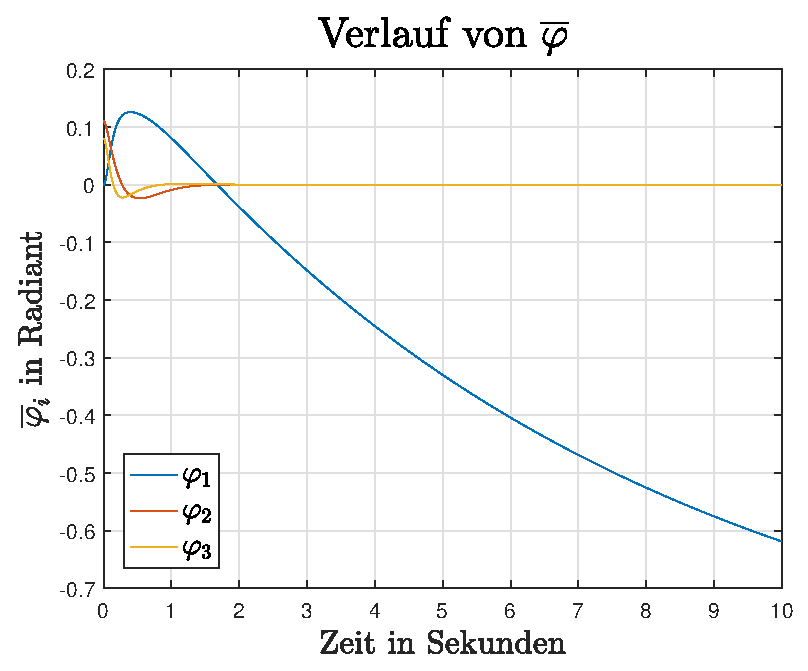
\includegraphics[width=0.45\linewidth]{img/lin_sim1_phi.eps}\hspace{1cm}
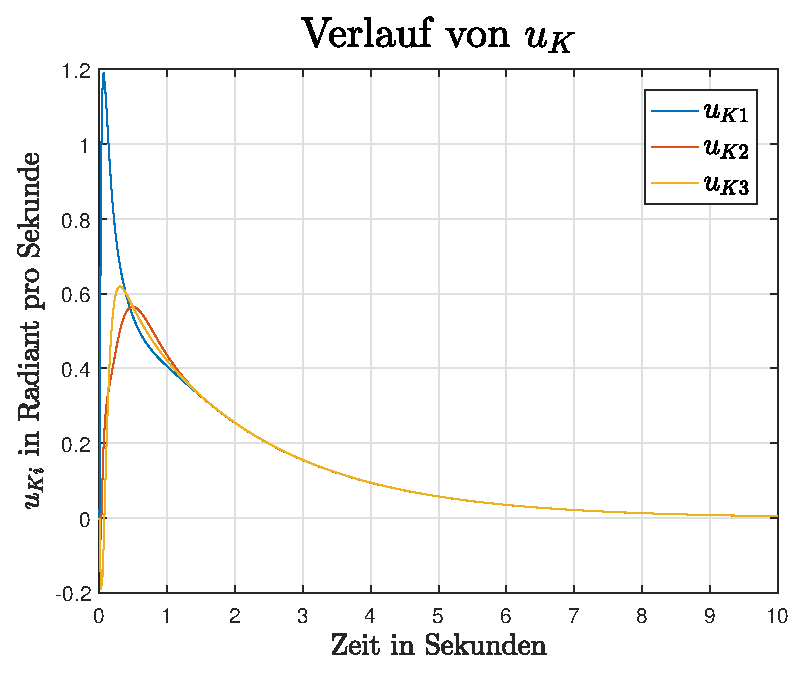
\includegraphics[width=0.45\linewidth]{img/lin_sim1_uk.eps}
\vspace{1cm}

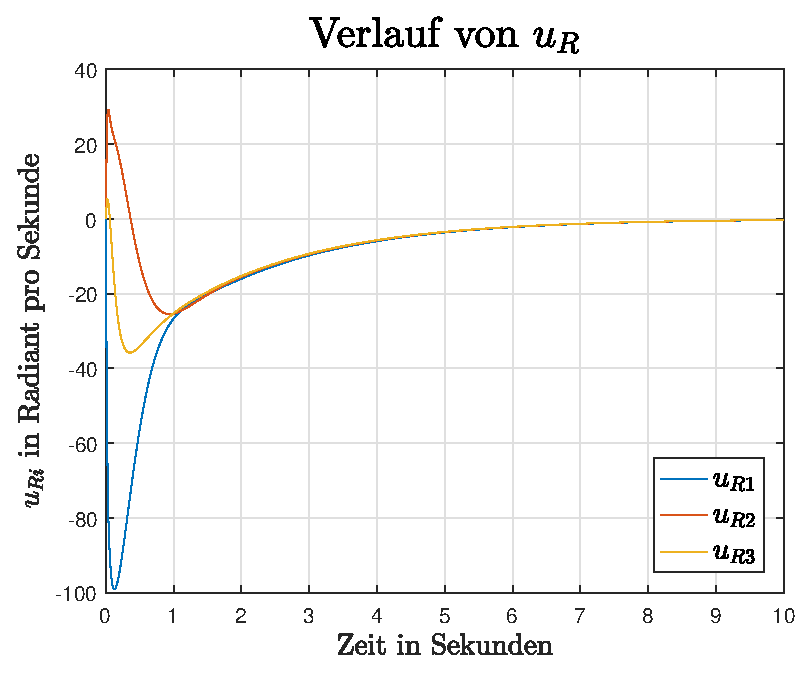
\includegraphics[width=0.45\linewidth]{img/lin_sim1_ur.eps}\hspace{1cm}
\includegraphics[width=0.45\linewidth]{img/lin_sim1_tm.eps}
\end{figure}
Die Simulation zeigt, dass alle Zustandsgrößen bis auf den Winkel $\varphi_1$ gegen null konvergieren. Folglich ist anzunehmen, dass der Zustand $\varphi_1$ nicht teil der Minimalrealisierung \textfrak{D}$_M$ ist. Diese Vermutung lässt sich mittels der Matrizen $\bs{C}_C$ und $\bs{A}_C$ bestätigen. Die erste Spalte der Matrix $\bs{C}_C$ ist ein Nullvektor und somit beeinflusst $\varphi_1$ den Ausgangsvektor $\bs{y}$ nicht. Eine solche Zustandsvariable wird auch als nicht ausgangsverbunden bezeichnet. Des weiteren hat der Zustand $\varphi_1$ keine Auswirkung auf die Systemdynamik. Dies ist auf die erste Spalte der Systemmatrix $\bs{A}_C$
\begin{equation}
\bs{A}_C(:,1) = \begin{bmatrix}
\bs{0}^{3\times 1} \\ \left[\bs{I}^{-1}_K\cdot \Delta\bs{T}_G\right](:,1)\\ \bs{0}^{3\times 1}
\end{bmatrix} = \bs{0}^{9\times 1}
\end{equation}
zurückzuführen, welche ebenfalls ein Nullvektor ist. Hieraus lässt sich schließen, dass es sich bei dem Winkel $\varphi_1$ um den nicht beobachtbaren Zustand $x_{\overline{B}}$ handelt. Dies wird auch von der Struktur der inversen Transformationsmatrix
\begin{equation}
\bs{T}^{-1}_K = \begin{bmatrix}
\bs{0}^{8\times 1} & \bs{T}^{-1}_K(2:9,2:9) \\
1 & \bs{0}^{1\times 8}
\end{bmatrix}
\end{equation}
bestätigt, welche $\varphi_1$ in $x_{\overline{B}}$ abbildet.

Mit Hilfe der Matrix $\bs{T}^{-1}_K$ kann auch der nicht steuerbare Zustand $x_{\overline{S}}$ interpretiert werden. Die zugehörige Zeile
\begin{equation}
\bs{T}^{-1}_K(8,:) \approx \begin{bmatrix}
0 & 0 & 0 & 0,5 & 0,5 & 0,7 & 0,01 & 0,01 & 0,01
\end{bmatrix}
\end{equation}
bildet den Zustandsvektor $\bs{x}$ in die Variable $x_{\overline{S}}$ ab. Diese ist somit eine Linearkombination der Geschwindigkeiten $\bs{u}_K$ und $\bs{u}_R$. Dieser Umstand erklärt auch das asymptotische Verhalten des Zustandvektors in der vorherigen Simulation. Da $\bs{u}_K(0)=\bs{u}_R(0)=\bs{0}$ und somit $x_{\overline{S}}(0)=0$ galt, kam die Grenzstabilität des nicht steuerbaren Zustandes nicht zum Tragen. Wird der Anfangszustand $\bs{x}(0)$ so angepasst, dass $x_{\overline{S}}(0)\neq \bs{0}$ gilt, ergibt sich das folgende Simulationsergebnis.
\clearpage
\begin{figure}[h]
\centering
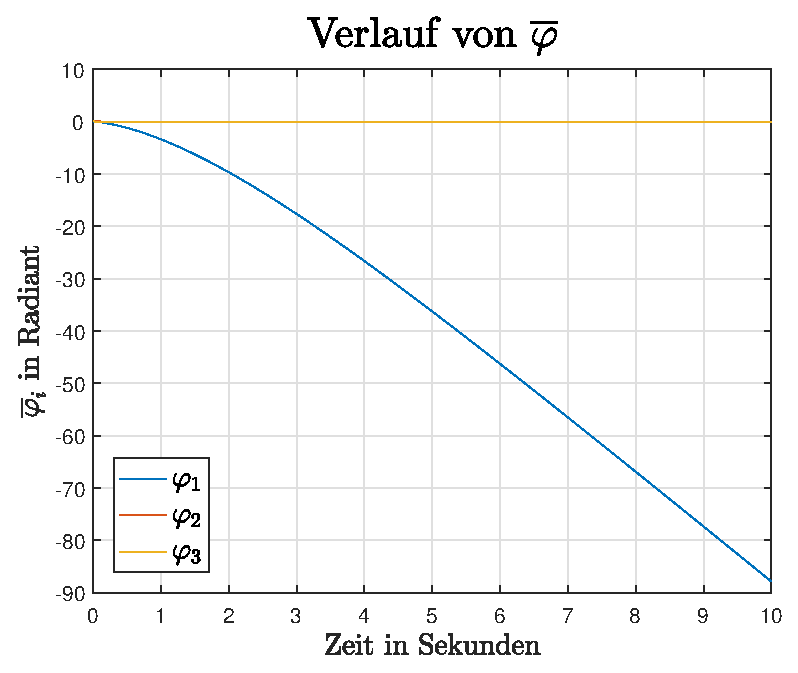
\includegraphics[width=0.45\linewidth]{img/lin_sim2_phi.eps}\hspace{1cm}
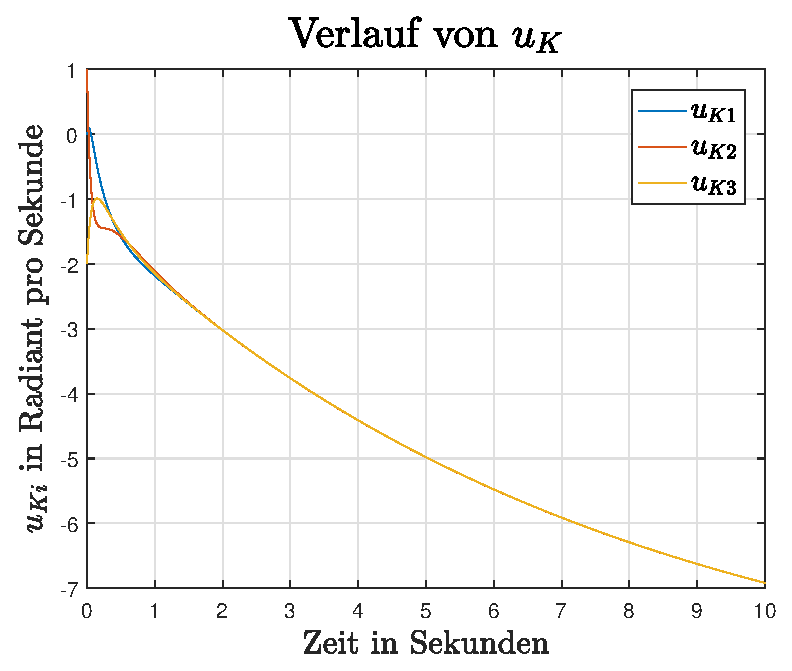
\includegraphics[width=0.45\linewidth]{img/lin_sim2_uk.eps}
\vspace{1cm}

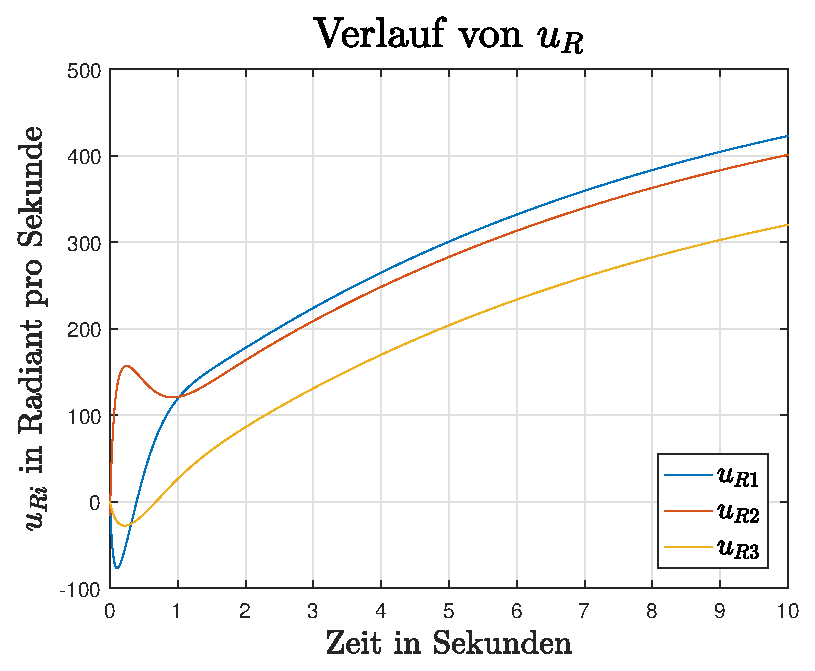
\includegraphics[width=0.45\linewidth]{img/lin_sim2_ur.eps}\hspace{1cm}
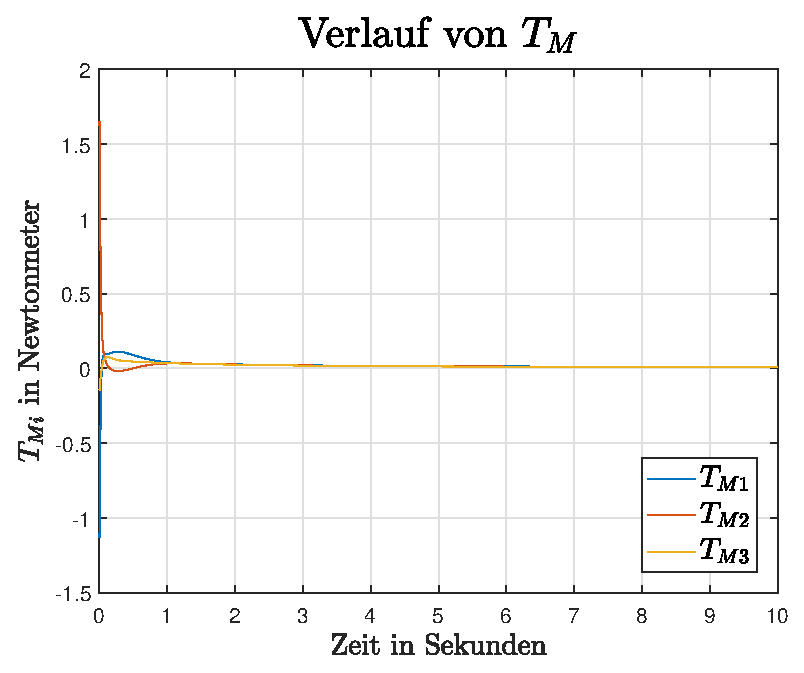
\includegraphics[width=0.45\linewidth]{img/lin_sim2_tm.eps}
\end{figure}
Die Simulation zeigt, dass die Winkel $\varphi_2$ und $\varphi_3$ nach wie vor asymptotisch stabil sind. Allerdings konvergieren die Winkelgeschwindigkeiten $\bs{u}_K$ gegen den gleichen Endwert $u_{Ke}\neq 0$. Mittels der Winkelgeschwindigkeit
\begin{equation}
\vel{A}{\omega}{K} = \vecBS{K}{u_{K1}}{u_{K2}}{u_{K3}}
\end{equation}
bedeutet der Endwert $u_{Ke}$, dass der Würfel mit einer konstanten Winkelgeschwindigkeit um seine Hauptdiagonale rotiert. Ebenso konvergieren die Geschwindigkeiten der Schwungmasse $\bs{u}_R$ und die Stellgrößen gegen einen von Null verschiedenen Endwert. Dieser Umstand kann an Hand des Systems \textfrak{D}$_K$ erklärt werden. Der Unterraum \textfrak{D}$_M$ ist im geschlossenen Regelkreis asymptotisch stabil. Allerdings wirkt der nicht steuerbare Zustand $x_{\overline{S}}$ proportional zu dem Vektor $\bs{a}_{M/\overline{S}}$ auf $\bs{x}_M$ ein.
\begin{equation}
\bs{x}_M(k+1) = \left(\bs{A}_M-\bs{B}_M\cdot \bs{K}_M\right)\cdot \bs{x}_M(k) + \bs{a}_{M/\overline{S}}\cdot \sigma(t)\cdot x_{\overline{S}}(0)
\end{equation}
Mit Hilfe des Endwertsatzes kann das Konvergenzverhalten bestimmt werden.
\begin{equation}
\begin{split}
z\cdot \bs{X}_M(z) &= \left(\bs{A}_M - \bs{B}_M\cdot \bs{K}_M\right)\cdot \bs{X}_M(z)  + \bs{a}_{M/\overline{S}}\cdot X_{\overline{S}}(z)
\\
\leftrightarrow \bs{X}_M(z) &= \left[z\cdot \bs{I} - \left(\bs{A}_M - \bs{B}_M\cdot \bs{K}_M\right) \right] ^{-1} \cdot \bs{a}_{M/\overline{S}}\cdot \underbrace{X_{\overline{S}}(z)}_{= \frac{z}{z-1}\cdot x_{\overline{S}}(t=0)}
\end{split}
\end{equation}
\begin{equation}
\lim_{k\rightarrow\infty} \bs{x}_M(k) = \lim_{z\rightarrow 1}(z - 1)\bs{X}_M(z) \equiv\bs{x}_{M,end}
\end{equation}
Wird der Zustandsvektor $\bs{x}_{K,end}$ aus den Endwerten der Teilsysteme zusammengesetzt kann dieser in den ursprünglichen Zustandsraum transformiert werden.
\begin{equation}
\begin{split}
\bs{x}_{end} &= \bs{T}_K\cdot \begin{bmatrix}
\bs{x}_{M,end} \\ x_{\overline{S}} \\ x_{\overline{B}}
\end{bmatrix} 
\\
&= \begin{bmatrix}
\varphi_1 & 0 & 0 & 5{,}4 x_{\overline{S}} & 5{,}4 x_{\overline{S}} & 5{,}4x_{\overline{S}} & -306{,}9 x_{\overline{S}} & -298{,}2 x_{\overline{S}} & -272{,}1 x_{\overline{S}}
\end{bmatrix}^T
\end{split}
\end{equation}
Dieses Ergebnis besagt, dass das System des Würfels ein Ruhelagenkontinuum besitzt. Die Winkel $\overline{\varphi}_2$ und $\overline{\varphi}_3$ konvergieren stets gegen null, was der aufrechten Position des Würfels auf einer Ecke entspricht. Allerdings rotiert der Würfel dabei mit einer konstanten, von $x_{\overline{S}}$ abhängigen Geschwindigkeit um seine Raumdiagonale. Des weiteren rotieren die drei Schwungmassen mit einer konstanten Endgeschwindigkeit, welche ebenfalls von $x_{\overline{S}}$ abhängt. In diesem Zusammenhang kann auch die nicht Steuerbarkeit des Zustandes $x_{\overline{S}}$ erklärt werden. Angenommen der Würfel rotiert in einer Ruhelage des Kontinuums mit einer konstanten Winkelgeschwindigkeit
\begin{equation}
\vel{A}{\omega}{K} = \vecBS{K}{u_{end}}{u_{end}}{u_{end}}\,.
\end{equation}
Nun ist es zwar möglich diese Rotation durch ein parallel gerichtetes Motormoment
\begin{equation}
\bs{T}_M = \vecBS{K}{T}{T}{T}
\end{equation}
zu beeinflussen, allerdings werden dadurch zwangsläufig die Winkelgeschwindigkeiten $\bs{u}_R$ der Schwungmassen beeinflusst. Somit ist es nicht möglich die Rotation des Würfels um seine Raumdiagonale unabhängig von der Bewegung der Schwungmassen zu beeinflussen, was wiederum gegen die Forderung der vollständigen Steuerbarkeit eines Systems verstößt. Dieses Ergebnis ist kritisch zu betrachtet, da hier lediglich ein linearisiertes System untersucht wurde. Um eine finale Aussage über die Steuerbarkeit des Systems zu treffen, müssen dessen nicht lineare Bewegungsgleichung auf geprüft werden. Da es sich bei dem Würfel um ein eingangslineares System handelt ist dessen Prüfung auf Steuerbarkeit analytisch möglich [Adamy, S.155ff]. Diese Untersuchung wird in dieser Arbeit allerdings nicht durchgeführt, da an der realen Regelstrecke lediglich Anfangszustände mit
\begin{equation}
\bs{\overline{\varphi}} \neq \bs{0} \hspace{35pt} \bs{u}_K \approx \bs{0} \hspace{35pt} \bs{u}_R \approx \bs{0}
\end{equation}
untersucht werden und der nicht steuerbare Zustand $x_{\overline{S}}$ somit nicht besonders ins Gewicht fällt.

\ifx\FORMAT\undefined
\end{document}
\fi


\ifx\FORMAT\undefined
\documentclass[11pt]{book}
\usepackage{amsmath,mathtools}
\usepackage[utf8]{inputenc}
\usepackage[ngerman]{babel}
\usepackage[T1]{fontenc}
\usepackage{lmodern}
\usepackage{acronym}
\usepackage{graphicx} 
\usepackage{epstopdf}
\usepackage{svg}
\usepackage{multirow}
\usepackage{amssymb}
\usepackage{trfsigns}
\usepackage{setspace}
\usepackage{yfonts}
\usepackage{nomencl}
\usepackage{float}
\usepackage{subfig}
\usepackage{scrpage2}
\usepackage{afterpage}
\usepackage{longtable}

\onehalfspacing


%Hyperlinks package, links aus inhaltsverzeichnis
\usepackage{hyperref}
\hypersetup{
    colorlinks=false, %set true if you want colored links
    linktoc=all,
    linkbordercolor = {white},
    citecolor = {white},
    allbordercolors = {white},
}
%Blattformatierung
\usepackage{geometry}
\geometry{a4paper, top=25mm, left=30mm, right=25mm, bottom=20mm}

%Listing
\usepackage{courier}
\usepackage{listings}
\usepackage{color}
 \lstset{
   frame=tb,
   framexleftmargin=2.5em,
   basicstyle=\small\linespread{0.9}\bfseries\ttfamily,
   emph={square}, 
   emphstyle=\color{blue}\texttt,
   emph={[2]root,base},
   emphstyle={[2]\color{yac}\texttt},
   showstringspaces=false,
   flexiblecolumns=false,
   tabsize=2,
   numbers=left,
   numberstyle=\small\bfseries\ttfamily,
   numberblanklines=false,
   stepnumber=1,
   numbersep=10pt,
   xleftmargin=25pt
 }
 
 \def\presuper#1#2%
	{\mathop{}%
	\mathopen{\vphantom{#2}}^{#1}%
	\kern-\scriptspace%
	#2}
%Display vecotr in a reference frame
\newcommand{\vecBS}[4]{\presuper{#1}{\begin{pmatrix}
#2 \\ #3 \\ #4
\end{pmatrix}}}
%Boldsymbol shortcut
\newcommand{\bs}[1]{\boldsymbol{#1}}
%Bezugssystemdefinition
\newcommand{\defBS}[1]{\{#1\} [ \bs{e}_{{#1}_1},\bs{e}_{{#1}_2}, \bs{e}_{{#1}_3} ]}
%Projektionsmatrix
\newcommand{\pMat}[2]{\presuper{#1}{\bs{P}}^{#2}}
%Differenation in Respekt zu BS
\newcommand{\diffIn}[3]{\frac{\presuper{#1}{d{#2}}}{d#3}}
\newcommand{\partialDiffIn}[3]{\frac{\presuper{#1}{\partial{#2}}}{\partial #3}}
%Geschwindigkeit/Beschleunigung
\newcommand{\vel}[3]{\presuper{#1}{\bs{#2}}^{#3}}

%Rightarrow with spaceing
\newcommand{\rArrow}{\hspace{5pt}\rightarrow\hspace{5pt}}
%Inneres Produkt
\newcommand{\inProd}[2]{\langle {#1}, {#2} \rangle}
\begin{document}
\fi

\chapter{Erfassung der Zustandsgrößen}
\newpage
\section{Bestimmung der Winkel $\varphi_i$}
Ein relevantes Problem stellt die Bestimmung der Winkel $\bs{\varphi}$ dar welche nur indirekt über die Beschleunigungssensoren ermittelt werden können. Die Messwerte $\bs{s}$ der Beschleunigungssensoren setzten sich aus der resultierenden Beschleunigung $\vel{A}{a}{S_i}$ und dem überlagerten Erdbeschleunigungsvektor $\bs{g}$ zusammen.
Zunächst wird der Fall betrachtet, dass die Messachsen der Sensoren mit dem körperfesten Bezugssystem $K$ zusammenfallen.
\begin{equation}
\bs{s}_i = \vel{A}{a}{S_i} + \bs{g}
\end{equation}
Unter der Annahme, dass der Würfel nicht bewegt wird verschwindet der Einfluss der Beschleunigung $\vel{A}{a}{S_i}$.
\begin{equation}
\bs{s}_i = \bs{g} = \norm{\bs{g}}\cdot \vecBS{K}{-c_{\varphi\idx2}\cdot c_{\varphi\idx3}}{c_{\varphi\idx2}\cdot s_{\varphi\idx3}}{-s_{\varphi\idx2}}
\end{equation}
Nun können die Winkel $\varphi\idx2$ und $\varphi\idx3$ aus den Komponenten des Messvektor $\bs{s}$ ermittelt werden.
\begin{equation}
\varphi_2 = -\text{asin}\left(\frac{\inProd{\bs{s}_i}{\bs{k}\idx3}}{\norm{\bs{g}}}\right)
\hspace{35pt}
\varphi_3 = -\text{atan}\left(\frac{\inProd{\bs{s}_i}{\bs{k}\idx2}}{\inProd{\bs{s}_i}{\bs{k}\idx3}}\right)
\end{equation}
Der Winkel $\varphi\idx1$ kann nicht aus dem Erdbeschleunigungsvektor ermittelt werden.  Jedoch schränkt dieser Umstand das Gesamtsystem nicht ein, da die Größe $\varphi\idx1$ keinen Einfluss auf die Systemdynamik hat. Um die Winkelschätzung auf den Fall des bewegten Würfels zu erweitern wird im nächsten Schritt die Beschleunigung $\vel{A}{a}{S_i}$ betrachtet. Da der Würfel eine rein rotatorische Bewegung durchführt genügt die Untersuchung der Winkelbeschleunigung und -geschwindigkeit [Kane S. 30].
\begin{equation}
\begin{split}
\vel{A}{a}{S_i} &= \vel{A}{\alpha}{K} \times \bs{r}_{S_i}  + \vel{A}{\omega}{K} \times \left( \vel{A}{\omega}{K}\times \bs{r}_{S_i} \right)
\\
&= \left[\vel{A}{\alpha}{K}\right]_\times \cdot \bs{r}_{S_i} + \left[\vel{A}{\omega}{K}\right]_\times \cdot \left(\left[\vel{A}{\omega}{K}\right]_\times \cdot \bs{r}_{S_i}\right)
\\
&= \left(\left[\vel{A}{\alpha}{K}\right]_\times + \left[\vel{A}{\omega}{K}\right]^2_\times \right) \cdot \bs{r}_{S_i}
\end{split}
\end{equation}
Wird nun die Summe der Beschleunigungswerte $\bs{s}_i$ berechnet, welche mit dem frei wählbaren Faktor $b_i \ \in R$ gewichtet werden, ergibt sich
\begin{equation}
\begin{split}
\sum^6_{i=1} b_i\cdot \bs{s}_i &= \sum^6_{i=1} \left[b_i\cdot \left(\kProdMat{\vel{A}{\alpha}{K}} + \kProdMat{\vel{A}{\omega}{K}}^2\right)\cdot \bs{r}_{\text{S}_i}  + b_i \cdot \bs{g}\right]
\\
&= \left(\kProdMat{\vel{A}{\alpha}{K}} + \kProdMat{\vel{A}{\omega}{K}}^2\right) \cdot \sum^6_{i=1}b_i\cdot \bs{r}_{\text{S}_i} + \bs{g}\cdot \sum^6_{i=1}b_i \,.
\end{split}
\end{equation}

Werden die Faktoren $b_i$ so gewählt, dass 
\begin{equation}
\sum^6_{i=1}b_i\cdot \bs{r}_{\text{S}_i} \hspace{35pt} \vert \hspace{15pt} \sum^6_{i=1}b_i \neq 0
\end{equation}
gilt, folgt
\begin{equation}
\sum^6_{i=1}b_i\cdot \bs{s}_i = \bs{g}\cdot \sum^6_{i=1} \hspace{15pt}\leftrightarrow\hspace{15pt} \bs{g} = \frac{\sum^6_{i=1}b_i\cdot\bs{s}_i}{\sum^6_{i=1}b_i}\,.
\end{equation}
Somit kann der Einfluss der resultierenden Beschleunigung $\vel{A}{a}{S_i}$ mittels der Faktoren $b_i$ eliminiert werden. Werden $n$ Sensoren verwendet, so muss für die Bestimmung der Faktoren $b_i$ das Gleichungssystem
\begin{equation}
\sum^n_{i=1}b_i\cdot \bs{r}_{\text{S}_i} = 0
\end{equation}
gelöst werden, wobei die Nebenbedingung
\begin{equation}
\sum^n_{i=1}b_i \neq 0
\end{equation}
zu beachten ist. Aus dieser Vorgehensweise können Rückschlüsse auf den Entwurf des Würfels gezogen werden. Sind die Ortsvektoren $\bs{r}_{S_i}$ linear abhängig genügen bereits zwei Sensoren um zwischen der resultierenden Beschleunigung $\vel{A}{a}{S_i}$ und der Erdbeschleunigung $g$ zu unterscheiden. Allerdings schränkt die Forderung nach linearer Abhängigkeiten die konstruktiven Möglichkeiten ein. Werden mehr als zwei Sensoren verwendet entfällt die Notwendigkeit der linearen Abhängigkeiten. Prinzipiell genügen drei Sensoren um die Einflüsse der Beschleunigung $\vel{A}{a}{S_i}$ zu eliminieren.
Die hier verwendeten Beschleunigungssensoren sind von zwei weiteren Einschränkungen betroffen. Zunächst ist die Empfindlichkeit der Messung in z-Richtung gegenüber den x- und y-Achsen geringer, weshalb lediglich die letzteren verwendet. Des weiteren stimmen die Messachsen der Sensoren nicht mit dem körperfesten Bezugssystem $K$ überein. Um diese Umstände im Modell auszudrücken werden die drei Messachsen des Sensors als Bezugssystem $S_i$ interpretiert. Unter der Annahme, dass die Messachsen und Vektoren $\bs{k}_i$ paarweise orthogonal zueinander stehen kann die Projektionsmatrix $\pMat{S_i}{K}$ aus dem Aufbau bestimmt werden. Zusätzlich wird die dritte Spalte $\pMat{S_i}{K}$ durch den Nullvektor ersetzt um die Vernachlässigung der z-Messwerte darzustellen.
\begin{equation}
\bs{s}_1 = \begin{bmatrix} 0 & 1 & 0 \\ 1 & 0 & 0 \\ 0 & 0 & 0\end{bmatrix}\cdot \presuper{S\idx1}{\bs{s}}\idx1 = \vecBS{K}{\inProd{\bs{s}_1}{\bs{k}_1}}{\inProd{\bs{s}_1}{\bs{k}_2}}{0} \hspace{25pt}
\bs{s}_2 = \begin{bmatrix} 0 & 1 & 0 \\ 1 & 0 & 0 \\ 0 & 0 & 0\end{bmatrix}\cdot \presuper{S\idx2}{\bs{s}}\idx2 = \vecBS{K}{\inProd{\bs{s}_2}{\bs{k}_1}}{\inProd{\bs{s}_2}{\bs{k}_2}}{0}
\end{equation}
\begin{equation}
\bs{s}_3 = \begin{bmatrix}
0 & 0 & 0 \\ 0 & 1 & 0 \\ 1 & 0 & 0
\end{bmatrix}\cdot \presuper{S\idx3}{\bs{s}}\idx3 = \vecBS{K}{0}{\inProd{\bs{s}_3}{\bs{k}_2}}{\inProd{\bs{s}_3}{\bs{k}_3}}\hspace{25pt}
\bs{s}_4 = \begin{bmatrix}
0 & 0 & 0 \\ 0 & 1 & 0 \\ 1 & 0 & 0
\end{bmatrix}\cdot \presuper{S\idx4}{\bs{s}}\idx4 = \vecBS{K}{0}{\inProd{\bs{s}_4}{\bs{k}_2}}{\inProd{\bs{s}_4}{\bs{k}_3}}
\end{equation}
\begin{equation}
\bs{s}_5 = \begin{bmatrix}
1 & 0 & 0 \\ 0 & 0 & 0 \\ 0 & 1 & 0
\end{bmatrix}\cdot \presuper{S\idx5}{\bs{s}}\idx5 = \vecBS{K}{\inProd{\bs{s}_5}{\bs{k}_1}}{0}{\inProd{\bs{s}_5}{\bs{k}_3}}\hspace{25pt}
\bs{s}_6 = \begin{bmatrix}
1 & 0 & 0 \\ 0 & 0 & 0 \\ 0 & 1 & 0
\end{bmatrix}\cdot \presuper{S\idx6}{\bs{s}}\idx6 = \vecBS{K}{\inProd{\bs{s}_6}{\bs{k}_1}}{0}{\inProd{\bs{s}_6}{\bs{k}_3}}
\end{equation}
Da die z-Messwerte nicht verwendet werden gibt jeder Sensor nur die Beschleunigung in Richtung zweier Vektoren $\bs{k}_i$ wieder. Um dieses Problem zu beheben werden die Messwerte jeweils zweier Sensoren zu einem abstrakten Messvektor $\bs{\tilde{s}}_i$ zusammengefasst.
Um hierbei die Auswirkung der Beschleunigungen $\vel{A}{a}{S_i}$ darzustellen wird die Definition
\begin{equation}
\kProdMat{\vel{A}{\alpha}{K}} + \kProdMat{\vel{A}{\omega}{K}}^2 \equiv \bs{M} = \begin{bmatrix}
\bs{m}^T\idx1 \\ \bs{m}^T\idx2 \\ \bs{m}^T\idx3
\end{bmatrix}
\end{equation}
verwendet. Die Vektoren $\bs{m}^T_i$ werden mit dem Ortsvektor des zugehörigen Sensors multipliziert.
\begin{equation}
\begin{split}
\bs{\tilde{s}}\idx1 \equiv \begin{bmatrix}
s\idx{1y} \\ s\idx{1x} \\ s\idx{3x}
\end{bmatrix} = \begin{bmatrix}
\bs{m}^T\idx1 \cdot \bs{r}_{\text{S}\idx1} \\
\bs{m}^T\idx2 \cdot \bs{r}_{\text{S}\idx1} \\
\bs{m}^T\idx3 \cdot \bs{r}_{\text{S}\idx3}
\end{bmatrix} + \bs{g} &\hspace{35pt}
\bs{\tilde{s}}\idx2 \equiv \begin{bmatrix}
s\idx{2y} \\ s\idx{2x} \\ s\idx{4x}
\end{bmatrix} = \begin{bmatrix}
\bs{m}^T\idx1 \cdot \bs{r}_{\text{S}\idx2} \\
\bs{m}^T\idx2 \cdot \bs{r}_{\text{S}\idx2} \\
\bs{m}^T\idx3 \cdot \bs{r}_{\text{S}\idx4}
\end{bmatrix} + \bs{g}
\\
\bs{\tilde{s}}\idx3 \equiv \begin{bmatrix}
s\idx{5x} \\ s\idx{3y} \\ s\idx{5y}
\end{bmatrix} = \begin{bmatrix}
\bs{m}^T\idx1 \cdot \bs{r}_{\text{S}\idx5} \\
\bs{m}^T\idx2 \cdot \bs{r}_{\text{S}\idx3} \\
\bs{m}^T\idx3 \cdot \bs{r}_{\text{S}\idx5} 
\end{bmatrix} + \bs{g} &\hspace{35pt}
\bs{\tilde{s}}\idx4 \equiv \begin{bmatrix}
s\idx{6x} \\ s\idx{4y} \\ s\idx{6y}
\end{bmatrix} = \begin{bmatrix}
\bs{m}^T\idx1 \cdot \bs{r}_{\text{S}\idx6} \\
\bs{m}^T\idx2 \cdot \bs{r}_{\text{S}\idx4} \\
\bs{m}^T\idx3 \cdot \bs{r}_{\text{S}\idx6}
\end{bmatrix} + \bs{g}
\end{split}
\end{equation}
In dieser Darstellung werden die Vektoren $\bs{\tilde{s}}_i$ mit den Diagonalmatrizen
\begin{equation}
\bs{B}_i = \begin{bmatrix}
b_{i\text{x}} & 0 & 0 \\ 0 & b_{i\text{y}} & 0 \\ 0 & 0 & b_{i\text{z}}
\end{bmatrix}
\end{equation}
multipliziert um die Einflüsse der Beschleunigungen zu eliminieren. Für die Summe der Gewichteten Vektoren gilt
\begin{equation}
\sum^4_{i=1}\bs{B}_i\cdot \bs{\tilde{s}}_i = 
\begin{bmatrix}
\bs{m}^T\idx1\cdot \sum^4_{i=1}b_{i\text{x}}\cdot\bs{r}_{\tilde{\text{S}}_{\text{x}i}} \\
\bs{m}^T\idx2\cdot \sum^4_{i=1}b_{i\text{y}}\cdot\bs{r}_{\tilde{\text{S}}_{\text{y}i}} \\
\bs{m}^T\idx3\cdot \sum^4_{i=1}b_{i\text{z}}\cdot\bs{r}_{\tilde{\text{S}}_{\text{z}i}}
\end{bmatrix}
+ \sum^4_{i=1}\bs{B}_i\cdot \bs{g}
\end{equation}
Wenn nun die Matrizen $\bs{B}_i$ so gewählt werden, dass einerseits
\begin{equation}
\sum^4_{i=1} b_{i\text{x}}\cdot \bs{r}_{\tilde{\text{S}}_{\text{x}i}} = 0
\hspace{35pt}
\sum^4_{i=1} b_{i\text{y}}\cdot \bs{r}_{\tilde{\text{S}}_{\text{y}i}} = 0
\hspace{35pt}
\sum^4_{i=1} b_{i\text{z}}\cdot \bs{r}_{\tilde{\text{S}}_{\text{z}i}} = 0
\end{equation}
und andererseits
\begin{equation}
\text{det}\left(\sum^4_{i=1}\bs{B}_i\right) \neq 0
\end{equation}
gelten, ergibt sich für die Summe der Messvektoren $\bs{\tilde{\text{s}}}_i$
\begin{equation}
\sum^4_{i=1}\bs{B}_i\cdot\bs{\tilde{\text{s}}}_i = \sum^4_{i=1}\bs{B}_i\cdot \bs{g} \hspace{15pt}\leftrightarrow\hspace{15pt}
\bs{g} = \left(\sum^4_{i=1}\bs{B}_i\right)^{-1}\cdot \sum^4_{i=1}\bs{B}_i\cdot\bs{\tilde{s}}_i \,.
\end{equation}
Somit können die Einflüsse der Beschleunigungen $\vel{A}{a}{S_i}$ auf die Messwerte auch bei den Messvektoren $\bs{\tilde{s}}_i$ eliminiert werden.
\newpage
\section{Komplementärfilter für die Winkel $\bs{\varphi}$}
Im Rahmen der Vorarbeit hat sich gezeigt, dass die Messwerte der Beschleunigungssensoren von Störsignalen betroffen sind. Die Sensoren reagieren empfindlich auf hochfrequente Störsignale wie z.B. den Vibrationen des Würfelgehäuses, welche von den Motoren verursacht werden. Um den Einfluss dieser Störgrößen zu minimieren wurde ein Komplementärfilter verwendet. Hierfür wird das Signal $\varphi$ aus zwei Quellen gewonnen, welche über das Komplementärfilter zusammengeführt werden. Einerseits kann eine Schätzung
\begin{equation}
\varphi_A = \varphi + v_A
\end{equation}
aus den Beschleunigungssensoren gewonnen werden, wobei $v_A$ das überlagerte Störsignal bezeichnet. Hierbei ist anzunehmen, dass es sich um ein hochfrequentes Signal handelt. Andererseits wird die Winkelgeschwindigkeit $\dot{\varphi}$ mittels der Drehratensensoren bestimmt. Über das Integral der Messwerte kann der Winkel
\begin{equation}
\varphi_G = \int \dot{\varphi} + \hat{\dot{\varphi}}\ dt = \varphi + v_G 
\end{equation}
bestimmt werden. Das Störsignal $v_G$ geht aus der Integration der systematischen Messabweichung $\hat{\dot{\varphi}}$ hervor. Da die Messabweichung $\hat{\dot{\varphi}}$ lediglich geringe Werte annimmt, handelt es sich bei $v_G$ um ein niederfrequentes Störsignal.

In dem Komplementärfilter werden die beiden Signale $\varphi_A$ und $\varphi_G$ addiert. Wobei $\varphi_A$ zuvor mit einem Tiefpass gefiltert wird um das hochfrequente Störsignale $v_A$ zu eliminieren. Parallel wird $\varphi_G$ mittels eines Hochpasses gefiltert um das niederfrequente Signal $v_G$ zu dämpfen. Der Tief- und Hochpass werden jeweils als IIR-Filter erster Ordnung mit identischer Zeitkonstante $\tau$ entworfen.
\begin{figure}[h!]
\includegraphics[width=1\linewidth, trim={2cm 7.5cm 4cm 3.5cm}, clip]{img/CompFilter}
\label{bsb_kompfilter}
\caption{Blockschaltbild Komplementärfilter, Quelle: eigene Darstellung}
\end{figure}

Für das resultierende Signal $\varPhi_C(s)$ folgt aus dem Blockschaltbild (\ref{bsb_kompfilter})
\begin{equation}
\begin{split}
\varPhi_C(s) &= \frac{1}{\tau \cdot s + 1}\cdot \varPhi_A(s) + \frac{\tau \cdot s}{\tau\cdot s + 1}\cdot \varPhi_G(s)
\\
&= \frac{1}{\tau\cdot s}\cdot \left[\varPhi(s) + V_A(s)\right] + \frac{\tau\cdot s}{\tau\cdot s + 1}\cdot \left[\varPhi(s) + V_G(s)\right]
\\
&= \varPhi(s) + \frac{1}{\tau\cdot s}\cdot V_A(s) + \frac{\tau\cdot s}{\tau\cdot s + 1}\cdot V_G(s) \,.
\end{split}
\end{equation}
Wird die Zeitkonstante $\tau$ nun so gewählt werden, dass die Störsignale $v_A$ und $v_G$ durch das Tief- bzw. Hochpassfilter eliminiert werden, besteht das Ausgangssignal $\varphi_C$ des Komplementärfilters lediglich aus dem Nutzsignal $\varphi$. Von besonderer Bedeutung für den Regelkreis ist hierbei, dass das Nutzsignal $\varphi$ von keiner Phasenverschiebung betroffen ist.

Dieses Filterkonzept kann auf den Fall des auf einer Ecke stehenden Würfels übertragen werden. Hierbei sind die beiden Winkel $\varphi_2$ und $\varphi_3$ zu bestimmen. Die Ableitungen dieser Signale hängen von der Winkelgeschwindigkeit $\vel{A}{\omega}{K}$ ab, welche mittels der Drehratensensoren erfasst wird.
\begin{equation}
\begin{bmatrix}
\dot{\varphi}_2 \\ \dot{\varphi_3}
\end{bmatrix} = \underbrace{\begin{bmatrix}
s_{\varphi_3} & c_{\varphi_3} & 0
\\
\frac{-s_{\varphi_2}c_{\varphi_3}}{c_{\varphi_2}} & \frac{s_{\varphi_2}s_{\varphi_3}}{c_{\varphi_2}} & 1
\end{bmatrix}}_{\equiv \bs{\Delta\varPhi}}
\cdot 
\begin{bmatrix}
u_{K1}\\ u_{K2} \\ u_{K3}
\end{bmatrix}
\end{equation}
Wird die Matrix $\bs{\Delta\varPhi}$ linearisiert können die Ableitung $\dot{\varphi}_2$ und $\dot{\varphi}_3$ aus den Winkelgeschwindigkeiten $\bs{u}_K$ berechnet werden. Die Ergebnisse aus dem vorherigen Abschnitt werden genutzt um die Winkel $\varphi_2$ und $\varphi_3$ auf den Beschleunigungsmessungen basierend zu schätzen. Mit Hilfe zweier Komplementärfilter werden diese jeweils mit den Ableitungen $\dot{\varphi}_i$ fusioniert. Diese Vorgehensweise führt zu einer ausreichenden Signalgüte um das in Abschnitt (\ref{section_corner_balance_test}) dokumentierten Reglerverhalten zu erreichen. Allerdings zeigt dieser Anwendungsfall die Grenzen des Komplementärfilters auf. Einerseits ist das Filter auf Grund der Linearisierung auf einen lokalen Arbeitsbereich eingeschränkt. Die Linearisierung ist allerdings nötig, da die Ableitungen $\dot{\varphi}_i$ sowohl von den Winkeln $\varphi_i$ als auch den Winkelgeschwindigkeiten $u_{Ki}$ abhängen. Werden für die Berechnung der Matrix $\bs{\Delta\varPhi}$ die Ausgangssignale des Filters verwendet, ergibt sich eine nichtlineare Filteroperation. Des weiteren können die Störsignale $v_A$ und $v_G$ durch die Filter nicht vollständig eliminiert werden und beeinflussen somit ebenfalls die Berechnung der Matrix $\bs{\Delta\varPhi}$.

\newpage
\section{Beobachter zur Ermittlung von $\varphi$}
In dem letzten Abschnitt sind die Nachteile des Komplementärfilters aufgezeigt worden. Aus diesem Grund wird am Beispiel des auf einer Kante balancierenden Würfels ein Luenberger-Beobachter entworfen, um den Winkel $\varphi$ zu bestimmen. Hierfür wird wieder das System
\begin{equation}
\textfrak{D} \equiv \left\{ \begin{array}{ll}
\bs{x}(k+1) &= \bs{A}\cdot \bs{x}(k) + \bs{b}\cdot u(k)
\\
\bs{y}(k) &= \underbrace{\begin{bmatrix}
\bs{0}^{2\times 1} & \bs{I}^{2\times 2}
\end{bmatrix}}_{= \bs{C}} \cdot \bs{x}(k)
\end{array}\right.\,, \hspace{35pt} \bs{x}=\begin{bmatrix}
\varphi \\ u_K \\ u_R
\end{bmatrix}
\label{eq_edge_system}
\end{equation}
betrachtet, wobei lediglich die Zustandsgrößen $u_K$ und $u_R$ messbar seine. Aus dem Kalmankriterium ergibt sich, dass das System vollständig beobachtbar ist. D.h. der Verlauf der Zustandsgrößen kann aus dem Ausgangsvektor und der Eingangsgröße rekonstruiert werden. Hierfür wird ein Luenberger-Beobachter verwendet. Das Grundprinzip des Beobachters besteht darin einen Schätzwert $\bs{\hat{x}}$ aus dem Modell (\ref{eq_edge_system}) zu berechnen. Bei diesem Ansatz führt bereits eine minimale Abweichung zwischen dem Modell und dem realen System zu einem kontinuierlich zunehmenden Schätzfehler. Um diesen Fehler zu eliminieren wird das in der Regelungstechnik bewährte Konzept der Fehlerrückführung verwendet. Da der Zustandsvektor nicht messbar ist wird  die Differenz $\Delta \bs{y}$ der Ausgangsvektoren über die so genannte Beobachtermatrix $\bs{L}$ zurückgeführt.
\begin{figure}

\caption{Blockschaltbild des Luenberger-Beobachters, Quelle: eigene Darstellung}
\end{figure}
Um das Verhalten des Beobachters zu untersuchen wird der Schätzfehler $\bs{e}(k) = \bs{x}(k) - \bs{\hat{x}}(k)$ betrachtet.
\begin{equation}
\begin{split}
\bs{e}(k+1) &= \bs{x}(k+1) - \bs{\hat{x}}(k+1) \\
&= [\bs{A}\cdot \bs{x}(k) + \bs{B}\cdot \bs{u}(k)] - [\bs{A}\cdot \bs{\hat{x}}(k) + \bs{B}\cdot \bs{u}(k) +\bs{L}\bs{\hat{y}}(k)]
\\
&= [\bs{A}\cdot (\bs{x}(k) - \bs{\hat{x}}(k))] - \bs{L}\bs{C}\cdot[\bs{x}(k)-\bs{\hat{x}}(k)] 
\\
&= \bs{A}\cdot \bs{e}(k) - \bs{LC}\cdot\bs{e}(k) = (\bs{A}-\bs{LC})\cdot \bs{e}(k)
\end{split}
\end{equation}
Hieraus folgt, dass der Verlauf des Schätzfehlers $\bs{e}(k)$ ein geschlossenen System darstellt. Wird die Beobachtermatrix $\bs{L}$ so gewählt, dass die Eigenwerte der Systemmatrix $\bs{A}-\bs{LC}$ im Einheitskreis liegen konvergiert der Schätzfehler gegen null. Da die Eigenwerte durch die Transponierung einer Matrix nicht verändert werden, kann die Entwurfsaufgabe als
\begin{equation}
\left\vert \lambda_i\left\{\bs{A}^T-\bs{C}^T\bs{L}^T\right\}\right\vert \overset{!}< 1
\end{equation}
formuliert werden. Diese Problemstellung entspricht der Entwurfsaufgabe eines gewöhnlichen Zustandsreglers, weshalb die bereits vorgestellten Verfahren für den Reglerentwurf auch für die Bestimmung der Beobachtermatrix $\bs{L}$ verwendet werden können. Für diesen Anwendungsfall wird der Beobachter optimal im Sinne des quadratischen Gütekriteriums entworfen. Als Gewichtungsmatrix $\bs{R}$ wird die Kovarianzmatrix des Ausgangvektors $\bs{y}$ verwendet. Die Matrix $\bs{Q}$ wird empirisch ermittelt. Prinzipiell unterliegt der Beobachter keiner Stellgrößenbeschränkung, da die Rückführung von $\Delta\bs{y}$ digital berechnet wird. Allerdings wirkt ein Messrauschen proportional zu $\bs{L}$ auf den Schätzwert $\bs{\hat{x}}$ ein. Aus diesem Grund werden die Elemente der Gewichtungsmatrix $\bs{Q}$ möglichst klein gewählt. Die folgenden Abbildung zeigen den Verlauf des System, wobei der Regler mit Hilfe des geschätzten Zustandvektors $\bs{\hat{x}}$ berechnet wird. Die folgende Abbildung zeigt den Verlauf der Zustandsgrößen und der Stellgröße im geschlossenen Regelkreis, wobei der Regler mittels des geschätzten Zustandvektors $\bs{\hat{x}}$ berechnet wurde.
\begin{figure}[h!]
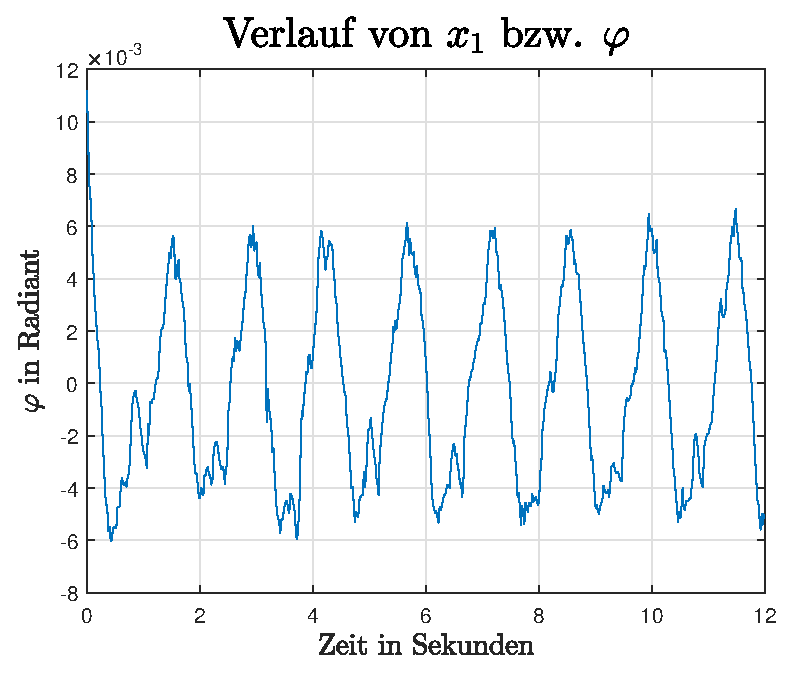
\includegraphics[width=0.45\linewidth]{img/edge_exp3_phi.eps}
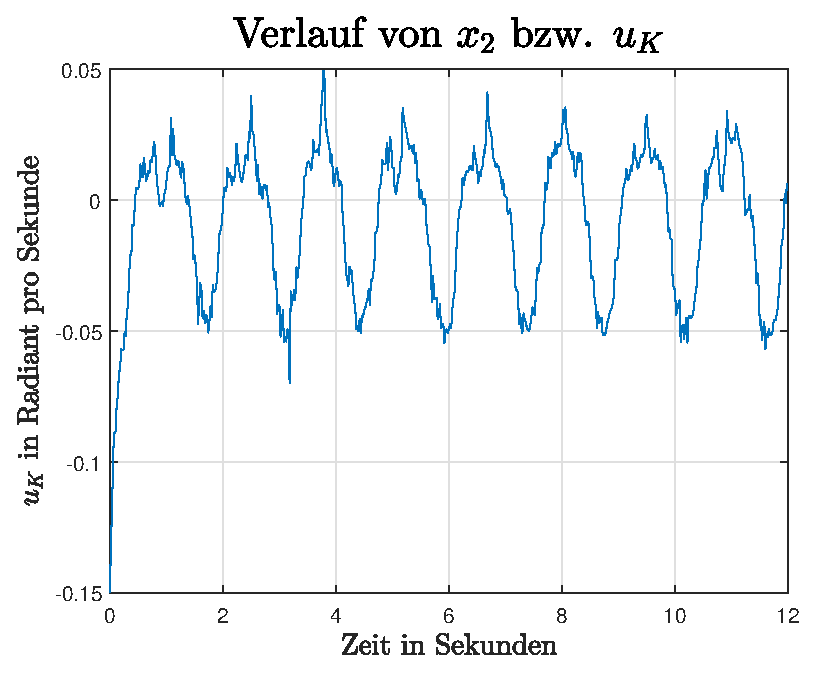
\includegraphics[width=0.45\linewidth]{img/edge_exp3_uk.eps}
\vspace{0.5cm}

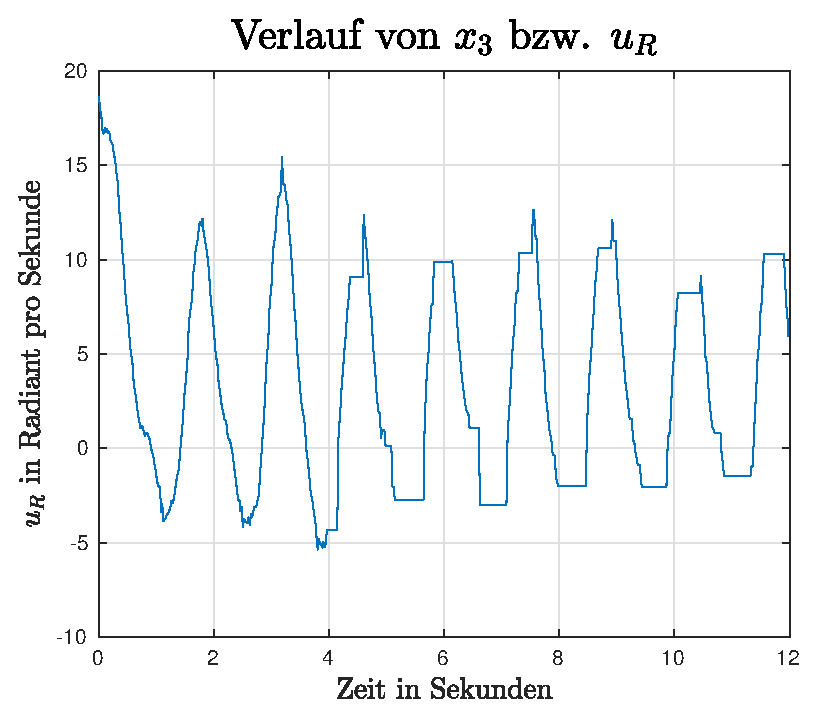
\includegraphics[width=0.45\linewidth]{img/edge_exp3_ur.eps}
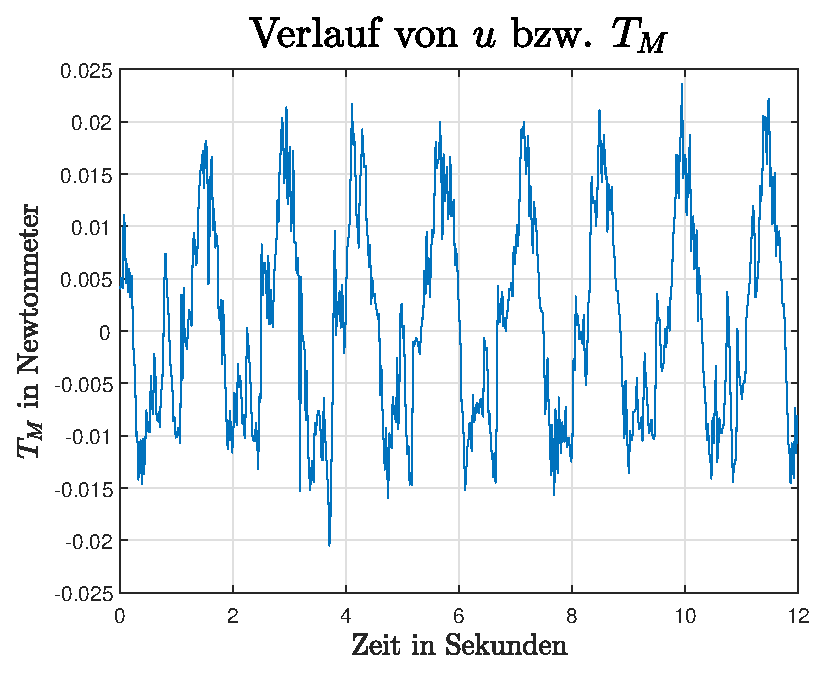
\includegraphics[width=0.45\linewidth]{img/edge_exp3_tm.eps}
\label{plots_phiobs}
\caption{Verlauf des geschätzten Zustandvektors und der Stellgröße, Quelle: eigene Darstellung}
\end{figure}

Der Versuch zeigt, dass das System mit dem Beobachter lediglich grenzstabil ist und mit einer konstanten Amplitude oszilliert. Eine mögliche Begründung für dieses Verhalten ist die Wahl der Beobachtermatrix. Um den Einfluss des Messrauschens zu minimieren wurde die Gewichtungsmatrix $\bs{Q}$ so gewählt, dass eine Beobachtermatrix mit relativ kleinen Elementen resultiert. Hieraus folgt, dass die Eigenwerte des Beobachters nahe an dem Einheitskreis liegen und somit bereits kleine Ungenauigkeiten in den Modellparametern genügen um grenzstabile Eigenwerte zu erhalten. Werden die Eigenwerte des Beobachters näher zu dem Urpsrung gerückt wird der Beobachter allerdings instabil, da das Messrauschen den Schätzwert $\bs{\hat{x}}$ zu stark beeinflusst. Dieses Problem ist darauf zurückzuführen, dass der Luenberger-Beobachter für ein deterministisches System entworfen wird und die stochastischen Störung lediglich indirekt bei dem Entwurfsverfahren berücksichtigt werden. Eine Lösung für dieses Problem stellt das Kalman-Filter dar, welches für die Beobachtung von linearen, zeitvarianten und stochastisch gestörten Systemen genutzt werden kann. Des weiteren bestehen Erweiterung wie das Extended-Kalman-Filter um das Konzept auf nichtlineare Systeme zu übertragen. 
Die Vorteile dieses Ansatz bestehen einerseits darin, dass mit einer Erweiterung auf nichtlineare Systeme ein global gültiges Schätzverfahren entsteht. Andererseits wird durch die Schätzung der Winkel $\varphi_i$ die Anzahl der benötigten Sensoren reduziert. Ebenso kann ein Kalman-Filter genutzt werden um die verrauschten Beschleunigungsmessungen mit den Winkelgeschwindigkeiten zu fusionieren. Im ersten Schritt ist allerdings eine Systemidentifikation und Parameterschätzverfahren durchzuführen, da eine mögliche Ursache für die verbleibende Schwingungen eine geringe Modellgüte ist. Derartige Fehler wirken sich ebenso negativ auf ein Kalman-Filter aus.


\ifx\FORMAT\undefined
\end{document}
\fi


\ifx\FORMAT\undefined
\documentclass[11pt]{book}
\usepackage{amsmath,mathtools}
\usepackage[utf8]{inputenc}
\usepackage[ngerman]{babel}
\usepackage[T1]{fontenc}
\usepackage{lmodern}
\usepackage{acronym}
\usepackage{graphicx} 
\usepackage{epstopdf}
\usepackage{svg}
\usepackage{multirow}
\usepackage{amssymb}
\usepackage{trfsigns}
\usepackage{setspace}
\usepackage{yfonts}
\usepackage{nomencl}
\usepackage{float}
\usepackage{subfig}
\usepackage{scrpage2}
\usepackage{afterpage}
\usepackage{longtable}

\onehalfspacing


%Hyperlinks package, links aus inhaltsverzeichnis
\usepackage{hyperref}
\hypersetup{
    colorlinks=false, %set true if you want colored links
    linktoc=all,
    linkbordercolor = {white},
    citecolor = {white},
    allbordercolors = {white},
}
%Blattformatierung
\usepackage{geometry}
\geometry{a4paper, top=25mm, left=30mm, right=25mm, bottom=20mm}

%Listing
\usepackage{courier}
\usepackage{listings}
\usepackage{color}
 \lstset{
   frame=tb,
   framexleftmargin=2.5em,
   basicstyle=\small\linespread{0.9}\bfseries\ttfamily,
   emph={square}, 
   emphstyle=\color{blue}\texttt,
   emph={[2]root,base},
   emphstyle={[2]\color{yac}\texttt},
   showstringspaces=false,
   flexiblecolumns=false,
   tabsize=2,
   numbers=left,
   numberstyle=\small\bfseries\ttfamily,
   numberblanklines=false,
   stepnumber=1,
   numbersep=10pt,
   xleftmargin=25pt
 }
 
 \def\presuper#1#2%
	{\mathop{}%
	\mathopen{\vphantom{#2}}^{#1}%
	\kern-\scriptspace%
	#2}
%Display vecotr in a reference frame
\newcommand{\vecBS}[4]{\presuper{#1}{\begin{pmatrix}
#2 \\ #3 \\ #4
\end{pmatrix}}}
%Boldsymbol shortcut
\newcommand{\bs}[1]{\boldsymbol{#1}}
%Bezugssystemdefinition
\newcommand{\defBS}[1]{\{#1\} [ \bs{e}_{{#1}_1},\bs{e}_{{#1}_2}, \bs{e}_{{#1}_3} ]}
%Projektionsmatrix
\newcommand{\pMat}[2]{\presuper{#1}{\bs{P}}^{#2}}
%Differenation in Respekt zu BS
\newcommand{\diffIn}[3]{\frac{\presuper{#1}{d{#2}}}{d#3}}
\newcommand{\partialDiffIn}[3]{\frac{\presuper{#1}{\partial{#2}}}{\partial #3}}
%Geschwindigkeit/Beschleunigung
\newcommand{\vel}[3]{\presuper{#1}{\bs{#2}}^{#3}}

%Rightarrow with spaceing
\newcommand{\rArrow}{\hspace{5pt}\rightarrow\hspace{5pt}}
%Inneres Produkt
\newcommand{\inProd}[2]{\langle {#1}, {#2} \rangle}
\begin{document}
\fi

\chapter{Software}
Wie bereits in den letzten Abschnitten erläutert wird der Regler als diskretes System implementiert. Deshalb spielt die verwendete Hardware und darauf ausgeführte Software eine zentrale Rolle. Dieser Umstand wird dadurch verstärkt, dass sämtliche Versuche, wie z.B. die Justierung der Sensoren, Systemidentifikation und Erprobung verschiedener Reglerkonzepte, in Form eines Programms durchgeführt werden. Aus diesem Grund widmet sich dieser Abschnitt dem Aufbau einer Software-Infrastruktur, welche die effiziente Entwicklung von mechatronischen Anwendungen ermöglicht.

\newpage
\section{Zielplattform, Sensorik und Aktorik}
In diesem Projekt wird ein \ac{BBB} in Kombination mit einer Linux-Distribution verwendet um die digitale Regelung zu realisieren. Die Plattform basiert auf einem AM335x Sitara ARM Cortex-A8 Prozessor, der mit einer Taktrate von 1GHz betrieben wird. Des weiteren steht eine single precision NEON FPU, für die Berechnung von Gleitkommaoperationen, zur Verfügung. Diese Rechnerarchitektur reduziert die nötige Rechenezit für gewöhnliche Filter- und Regelungsalgorithmen auf wenige Mikrosekunden. Somit kann die, durch die Rechnung resultierende Totzeit, des digitalen Systems bei dem Reglerentwurf vernachlässigt werden.
Das Linux-Betriebssystem bringt weitere Vorteile für die Entwicklung des Gesamtsymtems mit sich. Zunächst existiert eine Vielzahl von Werkzeugen für die Entwicklung von Embbeded-Linux-Anwendungen. Dadurch wird der nötige Zeitaufwand für die Implementierung des Reglerprogramms reduziert werden. Des weiteren kann bei der Entwicklung auf Pakete und Bibliotheken der Linux-Gemeinde zurückgegriffen werden. Somit können auch komplexe Subsysteme, wie z.B. der hier verwendete WebSocketServer, in das Gesamtsystem eigebettet werden. Zuletzt kann das Dateisystem genutzt werden um Konfigurationen für Filter- und Regleralgorithmen auszutauschen, wodurch die Erprobung von verschiedenen Reglerkonzepten vereinfacht wird. 
Allerdings muss der Einfluss des Betriebssystem auf das Zeitverhalten der Regelung kritisch betrachtet werden. Einerseits kann die Abtastung an äquidistanten Stützstellen nicht mehr garantiert werden. Anderseits entsteht durch die Verwendung von Linux-Treibern Verzögerungen, die zu weiteren Totzeiten führen. Deshalb beschäftigt sich der nächste Abschnitt mit der verwendeten Peripherie und deren softwareseitige Auswertung.

\subsection{Peripherie}
Auf dem Würfelgehäuse sind insgesamt sechs MPU9250-Module[Datenblatt MPU] montiert. Die Module besitzen jeweils einen Beschleunigungs- und Drehratensensor, welche genutzt werden um einen Teil des Zustandvektors zu bestimmen. Die Kommunikation zwischen den Sensormodulen und dem \ac{BBB} erfolgt über einen \ac{SPI}-Bus. Das das \ac{SPI}-Modul des \ac{BBB} nur einen \ac{CS}Pin besitzt wird dieser über einen AnalogSwitch[DatenBlatt] mit den Sensoren verbunden.
\begin{figure}[!h]
\centering
\includegraphics[width=0.7\linewidth]{img/SW_0_Sensoren_BSB.pdf}
\caption{Blockschaltbild Sensorkommunikation, Quelle: eigene Darstellung}
\end{figure}
Drei digitale Ausgänge des \ac{BBB} sind mit den Steuereingängen des Schalters verbunden um die \ac{CS}-Leitung auf den Ausgang des gewünschten Sensors zu legen.
Im Quellcode werden die Peripheriegeräte durch Klassen repräsentiert. Für die Steuerung der Digitalausgänge wird die Klasse \textit{CGPIO} implementiert, welche als Konstruktorargument die Nummer des zu konfigurierenden Pins entgegennimmt. Des weiteren betet sie Methoden zum Setzen bzw. Rücksetzen des Ausgangs. Hierfür wird die Schnittstelle des Treibers im Dateisystem verwendet. Zur Steuerung des Switches wird die Klasse \textit{CSwitch} aus drei Instanzen des Typs \textit{CGPIO} komponiert und implementiert die Methoden \textit{selectXi()} um die Schalterausgänge auszuwählen.
Analog wird für die Konfiguration und Auswertung der Sensoren die Klasse \textit{CMPU9250} implementiert. Zur Interaktion mit dem \ac{SPI}-Treiber wird die Posix-Funktion \textit{ioctl()} verwendet, welche zu einer kürzeren Ausführungszeit der Treiberaufrufe führt und im Vergleich zu der Dateisystemschnittstelle detaillierte Konfigurationsoptionnen bietet. Die Klasse nutzt die \ac{SPI}-Schnittstelle um die Sensoren in der \textit{init()}-Methode zu konfigurieren. Anschießend können über die Methode \textit{fetchData()} die aktuellen Beschleunigungs- und Winkelgeschwindigkeitswerte ausgelesen werden.

Die letztendliche Anwenderschnittstelle bietet die Klasse \textit{CSensorSystem}, welche aus einer Instanz des Typ \textit{CSwitch} und \textit{CMPU9250} komponiert wird. Im Konstruktur werden die sechs Sensoren initialisiert und anschließend über die Methode \textit{fetchSensorData()} ausgelesen. Die Daten werden in der Struktur \textit{SSensorData} gespeichert, welche Membervariablen für die Messwerte besitzt.
\begin{figure}[!h]
\centering
\includegraphics[width=0.7\linewidth]{img/SW_0_Sensoren_KD.pdf}
\caption{Klassendiagramm der Sensorschnittstelle, Quelle: eigene Darstellung}
\end{figure}

Die Stellgrößen der Regelung werden durch drei Motoren generiert, die jeweils über einen Treiberbaustein kontrolliert werden. Jeder Motortreiber ist mit zwei digitalen Ausgängen verbunden. Diese steuern die Freigabe und Drehrichtung des Motors. Die Vorgabe des Drehmoments erfolgt über ein \ac{PWM}-Signal. Zusätzlich erfassen die Motortreiber die Drehzahl und geben diese in Form eines Analogsignals an das \ac{BBB} zurück.
\begin{figure}[!h]
\centering
\includegraphics[width=0.7\linewidth]{img/SW_0_Motoren_BSB.pdf}
\caption{Blockschaltbild der Motoransteuerung, Quelle: eigene Darstellung} 
\end{figure}
Die Klasse \textit{CPWM} ermöglicht das Setzen eines Duty-Cycles, wobei die Treiberschnittstelle im Dateisystem verwendet wird. Eine Instanz dieser Klasse wird in \textit{CMotor} genutzt um das gewünschte Drehmoment einzustellen. Des weiteren werden zwei Instanz von \textit{CGPIO} genutzt um die Freigabe und Drehrichtung des Motors einzustellen. Für das Auslesen der \ac{ADC}-Werte wird ebenfalls eine Klasse \textit{C\ac{ADC}} angelegt. Da der Linux-Treiber für die Nutzung der AD-Wandler teilweise fehlerhaft ist wird ein alternative Vorgehensweise zur Nutzung der Peripherie genutzt. Hierbei wird mittels der Posix-Funktion \textit{mmap()} der Adressbereich der \ac{ADC}-Peripherie in den Userspace gelegt. Dadurch kann in der Anwendung direkt auf die \ac{ADC}-Register zugegriffen werden. Durch diesen Ansatz ergeben sich zwei Vorteile. Einerseits werden dem Nutzer keine Einschränkungen durch die Treiberschnittstelle aufgezwungen. Andererseits wird die nötige Zeit der AD-Wandlung durch den direkten Zugriff auf die Register reduziert. Allerdings ist diese Vorgehensweise mit einem größeren Implementierungsaufwand verbunden und wird deshalb nur genutzt wenn die Einschränkungen des Treibers nicht annehmbar sind.
die Klasse \textit{CSensorSystem} wird um eine Instanz von \textit{CADC} erweitert und umfasst somit die vollständige Sensorik des Systems. Um die Peripherie vollständig zu kapseln wird die Klasse \textit{CHardware} aus einer Instanz von \textit{CMotor} und \textit{CSensorSystem} komponiert.
\begin{figure}[!h]
\centering
\includegraphics[width=0.7\linewidth]{img/SW_0_Hardware_KD.pdf}
\caption{Klassendiagramm der Hardwareansteuerung, Quelle: eigene Darstellung}
\end{figure}
\newpage
\section{Implementierung des Signalflusses}
Im nächsten Schritt muss der Signalfluss implementiert werden. Hierfür wird ein Ansatz der Template-Metaprogrammierung verwendet, um ein einheitliches Konzept für die Umsetzung von Singalverarbeitungsalgorithmen zu schaffen. Ebenso soll das Konzept Änderung im Singalfluss ermöglichen, ohne dabei größere Eingriffe im Quellcode vornehmen zu müssen. Als Beispiel wird das folgende Blockschaltbild verwendet.
Zunächst wird eine, auf den Sensorwerten basierende, Zustandsschätzung durchgeführt. Dieser Vektor wird anschließend gefiltert und zur Berechnung des Reglers genutzt.
\begin{figure}[!h]
\centering
\includegraphics[width=\linewidth]{img/SW_1_Signalfluss_BSB.pdf}
\caption{Blockschaltbild des Signalflusses}
\end{figure}

Für die Implementierung werden die Signale als Datenobjekte implementiert. Das heßt es werden Strukturen oder Klassen entworfen, welche die Daten enthalten und ggf. Methoden für den Zugriff oder Bearbeitung bieten. Für dieses Beispiel repräsentieren die Strukturen \textit{SSensorData} und \textit{SStateVector} den Sensor- bzw. Zustandsvektor. Für die Modellierung der Stellgröße genügt eine \textit{float}-Variable.
\begin{lstlisting}[caption={Beispielhafte Implementierung eines Datenobjektes},captionpos=b]
struct SSensorData
{
	Float32 mS1;
	Float32 mS2;
	Float32 mS3;
};
struct SStateVector
{
	Float32 mX1;
	Float32 mX2;
};
using UType = Float32;
\end{lstlisting}
Die Systeme im Signalfluss werden als Klassen implementiert, die als Aktionsobjekte bezeichnet werden. Die Klassen werden nach dem folgenden Schema entworfen, wobei als Beispiel ein Objekt zur Filter Zustandsschätzung aufgezeigt wird.
\begin{lstlisting}[caption={Beispielhafte Implementierung eines Aktionsobjektes},captionpos=b]
class CStateEstimate
{
public:
	using InputType	 = SSensorData;
	using OutputType = SStateVector;
public:
	const OutputType& calcOutput(const InputType& input);
	const OutputType& getValue() const;
	...
private:	 
	OutputType mOutput;
};
\end{lstlisting}
Die Aktionsobjekte definieren zunächst ihren Ein- und Ausgangstyp. Die Berechnung des Systems erfolgt über die Methode \textit{calcOutput()}.
Nun müssen die Aktionsobjekte zu dem vorgegebenen Signalfluss zusammengefasst werden. Um diesen Schritt im Entwicklungsprozess zu erleichtern, soll ein Konzept implementiert werden, dem eine Typenliste der Aktionsobjekte übergeben wird und daraus das Blockschaltbild erzeugt.
Für die Implementierung der Typenliste wird der Ansatz nach [ModernCppDes] verwendet. Zunächst wird die leere Struktur \textit{CNullType} definiert, welche als Terminierungssymbol in der Typenliste fungiert. Die Liste wird mit Hilfe der Templatestruktur \textit{TTypeList} implementiert, welche als Parameter einen Anfangs- und Endtypen entgegennimmt.
\begin{lstlisting}[caption={Implementierung der Typenlist},captionpos=b]
struct CNullType{};

template<class HeadType, class TailType>
struct TTypeList
{
	using Head = HeadType;
	using Tail = TailType;
};
\end{lstlisting}
Die obige Implementierung unterstützt lediglich Listen der Länge zwei. Deshalb werden Makros verwendet, die rekursive Intanszierungen des Templates nutzen um die Listen beliebiger Länge zu erhalten. Mittels dieser Makros kann dann auch die Typenliste der Aktionsobjekte erzeugt werden.
\begin{lstlisting}[caption={Definition und Aufruf der Makors für verlängerte Typenlisten},captionpos=b]
#define TYPELIST_1(T1)         TTypeList<T1, CNullType>
#define TYPELIST_2(T1, T2) 	   TTypeList<T1, TYPELIST_1(T2)>
#define TYPELIST_3(T1, T2, T3) TTypeList<T1, TYPELIST_2(T2, T3)>
...
using ActionObjList = TYPELIST_3(CStateEstimate, CFilter, CController);
\end{lstlisting}
Um nun die Aktionstypen zu einem Signalfluss-Objekt zusammenzufügen, wird das Muster der linearen Typenhierachie nach  [ModernCppDesign] angewandt. Dessen Aufbau erinnert an eine verkettete Liste, wobei allerdings Typen durch Vererbung verknüpft werden. Die Templateklasse \textit{TActionHolder} wird als Träger für die Aktionsobjekte entworfen.\begin{lstlisting}[caption={Implementierung der Trägerklasse für Aktionsobjekte},captionpos=b]
template<class ActionObj, class Base>
class TActionHolder : public Base, public ActionObj
{
public:
	void calcOutput(const ActionObj::InputType& input)
	{
		ActionObj::calcOutput(input);
		Base::calcOutput(ActionObj::getValue());
	}
};
template<class ActionObj>
class TActionHodler<ActionObj, CNullType> : 
	public CNullType, public ActionObj
{
public:
	void calcOutput(const ActionObj::InputType& input)
	{
		ActionObj::calcOutput(input);
	}
};
\end{lstlisting}
Im allgemeinen Fall wird dem Template der Typ eines Aktionobjektes \textit{ActionObj} und eine beliebige Elternklasse \textit{Base} übergeben, die beide an \textit{TActionHolder} vererben. In der \textit{calcOutput()}-Methode wird zunächst die Berechnung des Aktionsobjektes durchgeführt und anschließend \textit{calcOutput()} der zweiten Elternklasse aufgerufen.

Des weiteren besteht eine Templatespezialisierung für den Fall, dass ein Aktionstyp und \textit{CNullType}, der das Ende der Typenliste signalisiert, übergeben werden. Nun wird in der \textit{calcOutput()}-Methode lediglich das Aktionsobjekt berechnet, da das Ende der Typenliste und somit des Signalflusses erreicht ist.

Die zweite Templateklasse ist \textit{TLinHierachy}, mit dem folgenden Prototyp.
\begin{lstlisting}[caption={Deklaration der Templateklasse für lineare Hierarchien},captionpos=b]
template<class TList,
         template<AtomicType, class Base> class Unit,
         class Root = CNullType>
class TLinHierachy;
\end{lstlisting}
Der erste Templateparameter ist die Typenliste, welche die zu generierende Typenhierachie vorgibt. Der zweite Parameter ist eine Templateklasse, die als Träger der Objekte aus der Typenliste agiert. In diesem Anwendungsfall wird die zuvor definierte Templateklasse \textit{TActionHolder} verwendet. Der letzte Parameter ist der Terminierungstyp der Hierarchie, welcher als Standardargument \textit{CNullType} übergeben wird. Analog zu \textit{TActionHolder} werden durch Spezialisierungen zwei Fälle unterschieden. Zunächst sei der Fall betrachtet, dass der Parameter \textit{TList} eine Typenliste aus zwei beliebigen Typen ist.
\begin{lstlisting}[caption={Erste Templatespezialisierung der linearen Hierarchie},captionpos=b]
template<class T1, 
         class T2, 
         template<class, class> class Unit, 
         class Root>
class TLinHierachy<TTypeList<T1, T2>, Unit, Root>
	: public Unit<T1, TLinHierachy<T2, Unit, Root> >
{};
\end{lstlisting}
Diese Instanziierung wird solange genutzt bist das Ende der ursprünglichen Typenliste erreicht ist. Die instantiierte Klasse von \textit{TLinHierachy}, ist eine leere Klasse die von \textit{Unit} erbt. \textit{Unit} wird wiederum mit \textit{TLinHierachy} instantiiert, wobei lediglich der zweite Parameter \textit{T2} übergeben wird. Dadurch wird die ursprüngliche Typenliste schrittweise abgearbeitet.
Die zweite Templatespezialisierung wird genutzt um die Generation am Ende der Typenliste zu terminieren. Dies ist der Fall wenn \textit{TLinHierachy} mit einer Typeliste der Länge eins instantiiert wird.
\begin{lstlisting}[caption={Zweite Templatespezialisierung der linearen Hierarchie},captionpos=b]
template<class T, template<class, class> class Unit, class Root>
class TLinHierachy<TYPELIST_1(T), Unit, Root>
	: public Unit<T, Root>
{};
\end{lstlisting}
Für das hier aufgeführte Beispiel ergibt sich die folgende Vererbungshierarchie.
\begin{figure}[!h]
\centering
\includegraphics[width=0.7\linewidth]{img/SW_1_Signalfluss_KD.pdf}
\caption{Klassendiagramm der generierten Hierarchie}
\end{figure}
Der Vorteil dieses Konzept, welches mit einem nicht zu vernachlässigenden Programmieraufwand verbunden ist, zeigt sich bei der letztendlichen Nutzung. Sind die Aktionsobjekte definiert können sie in wenigen Zeilen zu dem Signalfluss zusammengesetzt werden.
\begin{lstlisting}[caption={Anwendungsbeispiel der linearen Hierarchie},captionpos=b]
using ActionList = TYPELIST_3(CStateEstimate, CFilter, CController);
using SignalFlow = TLinHierachy<ActionList, TActionHandler>;
SignalFlow mySF;
\end{lstlisting}
Sollen nun im Projektverlauf einzelne Elemente ausgetauscht oder erweitert werden muss lediglich die Typendefinition von \textit{ActionList} geändert werden. Da die Hierarchie mittels Vererbung realisiert wird, können durch die Angabe des Namensraum die Methoden aller Elternklassen verwendet werden. Beispielsweise zeigt der folgende Ausschnitt die Abfrage aller berechneten Signale.
\begin{lstlisting}[caption={Beispiel für den Zugriff auf Aktionsobjekte in der Hierarchie},captionpos=b]
SStateVector x_estimate = mySF.CStateEstimate::getValue();
SStateVector x_filtered = mySF.CFilter::getValue();
UType        u          = mySF.CController::getValue();
\end{lstlisting}
Ebenso können zur Laufzeit konfigurierbare Elemente oder Verzweigungen implementiert werden. Angenommen zur Filterung sollen entweder ein Komplementär-Filter (\textit{CCompFilter}) oder ein Tiefpass erster Ordnung (\textit{CPT1}) genutzt werden. Dann kann eine Klasse \textit{CFilterSystem} aus diesen beiden komponiert werden, die zusätzliche Methoden zur Filterauswahl bietet.
\begin{lstlisting}[caption={Beispiel für die komponierte Aktionsobjekte},captionpos=b]
class CFilterSystem
{
public:
	using InputType  = SStateVector;
	using OutputType = SStateVector;
public:
	const OutputType& calcOutput(const InputType& input)
	{
		mCompFilter.calcOutput(input);
		mPT1Filter.calcOutput(input);
		
		return this->getValue();
	}
	const OutputType& getValue()
	{
		switch(mActiveFilter)
		{
			case EFilter::CompFilter:
				return mCompFilter.getValue();
			case EFilter::PT1Filter:
				return mPT1Filter.getValue();
			default:
				return input;
		}
	}
	void setFilter(EFilter filter)
	{
		mActiveFilter = filter;
	}
private:
	CCompFilter mCompFilter;
	CPT1        mPT1Filter;
	EFilter     mActiveFilter;
};
\end{lstlisting}
Analog können auch komplexere Verzweigungen realisiert werden, wobei \textit{TLinHierachy} zur Generation von Teilzweigen des Blockschaltbildes verwendet werden kann.
\newpage
\section{Komponentenarchitektur für mechatronische Anwendungen}
In dem letzten Abschnitt wurden die elementaren Funktionen des Regelkreises, wie die Peripherieinteraktion und der Signalfluss, implementiert. Um eine effiziente Versuchsdurchführung zu ermöglichen müssen allerdings weitere Funktionalitäten bereitstehen. Einerseits muss einzelne Elemente des Regelkreises während der Ausführung konfigurierbar sein. Beispielsweise soll zwischen unterschiedlichen Regler umgeschaltet werden und einzelne Parameter geändert werden können. Des weiteren müssen die gemessen und berechneten Werte des Signalflusses an einen Entwicklungsrechner übertragen werden. Dort werden die Daten visualisiert und für eine spätere Analyse gespeichert.
Folglich muss ein Kommunikationskonzept implementiert werden um Daten zwischen der Ziel- und Entwicklungsplattform auszutauschen. Um die Berechnung des Regelkreises und die Kommunikationsaufgaben voneinander zu trennen wird eine Komponentenarchitektur eingeführt. Die erste Komponente, welche als Regelungskomponente bezeichnet wird, führt die Berechnung des Signalflusses und die Interaktion mit den Peripheriegeräten durch. Des weiteren übernimmt sie die logische Steuerung der Versuchsabläufe. Die Kommunikationskomponente ist für die Verbindung mit dem Entwicklungsrechner verantwortlich und ermöglicht den Datenaustausch zwischen den beiden Plattform. Hierfür wird ein WebSocketServer verwendet (siehe Abschnitt...).
\begin{figure}[!h]
\centering
\includegraphics[width=\linewidth]{img/SW_1_KA_BSB.pdf}
\caption{Blockschaltbild Gesamtsystem, Quelle: eigene Darstellung}
\end{figure}
Durch die Verwendung der Komponentenarchitektur enstehen einige Vorteile. Zunächst können die beiden Komponenten in unterschiedlichen Threads ausgeführt werden. Dadurch wird die Bearbeitung der beiden Aufgabenbereiche zum Großteil entkoppelt. Der Datenaustausch zwischen den Komponenten reduziert sich auf eine kontrollierte Schnittstelle, wodurch die Fehleranfälligkeit des Gesamtsystems minimiert wird. Des weiteren können die Aufgaben priorisiert werden, da der Scheduler eine preemptive Round-Robin-Strategie verfolgt. Somit kann die Ausführung der Regelungskomponente, welche für die Bearbeitung der zeit- und sicherheitsrelevanten Aufgaben zuständig ist, gegenüber der Kommunikationseinheit priorisiert werden. Hieraus resultiert, dass das Zeitverhalten der Regelung als deterministisch angenommen werden kann. 

Für die Implementierung wird das Interface \textit{IRunnable} definiert, welches virtuelle Methoden zur Initialisierung und Ausführung der Komponenten vorschreibt. Diese Schnittstelle wird von der abstrakten Klasse \textit{AComponentBase} geerbt, welche Membervariablen zum Datenaustausch besitzt. Die letzendlichen Komponenten werden in Form der beiden Klassen \textit{CControlComp} und \textit{CCommComp} realisiert. Die Erzeugung der Threads erfolgt mit Hilfe der Klasse \textit{CThread}, deren Instanz als Trägerobjekte der Threads agieren.
\begin{figure}[!h]
\centering
\includegraphics[width=0.6\linewidth]{img/SW_1_KA_KD.pdf}
\caption{Klassendiagramm der Komponenten, Quelle: eigene Darstellung}
\end{figure}

Im nächsten Schritt muss ein Weg zum Datenaustausch zwischen den Komponenten etabliert werden. Einerseits müssen Messdaten und Signale aus dem Regelkreis von der Regelungs- and die Kommunikationseinheit gesendet werden, welche diese anschließend an den Host-PC weiterleitet. Andererseits werden die Steuerbefehle des Host-PCs von der Kommunikationskomponente empfangen und an die Regelungskomponente gereicht. Da in diesem Anwendungsfall lediglich Datenpakete versendet werden, die kleiner als 32 Byte sind, werden Nachrichten für deren Austausch verwendet. Die Nachrichten werden in Form der Klasse \textit{CMessage} implementiert, welche aus einem Datenfeld, einem Ereignis und einem Zeitstempel komponiert werden. Das Eregnis wird als Enumeration realisiert und gibt den Inhalt der Daten bzw. den jeweiligen Befehl wieder. Der Zeitstempel gibt den Abtastzeitpunkt der Signale aus dem Regelkreis wieder. 
\begin{lstlisting}
enum class EEvent
{
	DEFAULT_IGNORE = 0,
	ASDF = 1
}
class CMessage
{
public:
	EEvent getEvent() const;
	UInt8* getDataPtr();
	...
public:

private:
	static constexpr UInt32 sDataSize = 32U;

	EEvent  mEvent;
	Float32 mTime;	
	UInt8   mData[sDataSize];
};
\end{lstlisting}
Des weiteren besitzt die Klasse Methoden und Konstruktoren um die Datenfelder entsprechend zu füllen und auszulesen. Um die Nachrichten zu empfangen besitzen die Komponenten Eingangspuffer die als Queues implementiert werden. Die Erzeugung der Nachrichten wird von einem Proxy übernommen, der Methoden für die unterschiedlichen Ereignisse bereitstellt. Des weiteren kennt der Proxy die Queues der Komponenten und legt neue Nachrichten, in Abhängigkeit von dem jeweiligen Event, in die Eingangspuffers des zugehörigen Empfängers.
\begin{lstlisting}
class CProxy
{
	public:
		bool transmitStateVector(const StateVector& x);
		...
};
\end{lstlisting}
Mit Hilfe der Nachrichtenkommunikation kann auch das Ablaufschema der Komponenten verallgemeinert werden. Beim Starten der Threads werden die Komponenten zunächst über den Aufruf ihrer \textit{init()}-Methoden initialisiert, anschließend wird die \textit{run()}-Methode ausgeführt, welche in diesem Fall eine Endlosschleife darstellt. In einem Durchlauf wird geprüft ob neue Nachrichten vorhanden sind, ist dies der Fall wird die Nachricht über die \textit{dispatch()}-Methode verarbeitet. Andernfalls legt sich der Thread schlafen bis neue Nachrichten zur Verfügung stehen. Hieraus ergeben sich zwei Vorteile. Einerseits werden die Komponenten nach einem einheitlichen Konzept entworfen, lediglich die Implementierung der \textit{init()}- und \textit{dispatch()}-Methode unterscheiden sich, andererseits wird durch die Synchronisation der Komponenten deren Laufzeit reduziert.
\newpage
\section{Aufbau der Regelungskomponente}\label{section_controlcomp}
Die Aufgabe der Regelungskomponente besteht darin den Kontroll- und Signalfluss der verschiedenen Versuche zu steuern. Diese Umsetzung erfolgt mit Hilfe eines Zustandautomats, welcher die Trennung der Kontrolllogik und der auszuführenden Aktionen ermöglicht. Des Weiteren kann die Applikation bei diesem Ansatz problemlos durch weitere Versuche und Anwendungsfälle erweitert werden. 
Prinzipiell lässt sich der logische Ablauf der Komponente mit einem einfachen Zustandsdiagramm modellieren. Auf der obersten Ebene existiert ein \textit{Standby}-Zustand, der die Inaktivität der Komponente widerspiegelt. Außerdem enthält diese Ebene Zustände für die verschiedenen Versuche. Diese werden betreten, wenn die Komponente ein Event mit dem entsprechenden Befehl zur Ausführung des Versuchs erhält.
\begin{figure}[h!]
\centering
\includegraphics[width=0.7\linewidth]{img/SW_2_ControlComp_SC.pdf}
\caption{Zustandsdiagramm der Kontrol-Komponente}
\end{figure}
Ein solches Zustandsdiagramm kann z.B. mit einer objektorientierten Adaption der Methode von Samek \cite[S. 246 ff.]{Wietzke1} implementiert werden. Hierbei werden Zustände als Methoden der FSM realisiert, wobei für Oberzustände eigene Klassen entworfen werden, die wiederum Methoden für die jeweiligen Unterzustände besitzen. Die Referenzierung des aktuellen Zustandes erfolgt über einen Funktionenzeiger, der auf die Methode des entsprechenden Zustandes gerichtet ist. 

Als Basis der Typenhierachie dient die abstrakte Klasse \textit{AState}, welche den Zustandstypen als Methodenzeiger definiert, eine Standardimplementierung der \textit{dispatch()}-Methode vorgibt und statische Membervariablen deklariert, um die Verarbeitung interner Events zu ermöglichen.
\begin{lstlisting}[caption={Abstrakte Basisklasse für die Zustände},captionpos=b]
class AState
{
protected:
	using StatePtr = bool (AState::*)(CMessage&);
public:
	virtual bool onInitial(CMessage& msg) = 0;
	virtual bool dispatch(CMessage& msg);
protected:
	StatePtr mStatePtr;
	static constexpr StatePtr sInitial = 
			static_cast<StatePtr>(AState::onInitial);
	static CMessage sInternalQueue;
	static UInt32   sQueueSize;
};
\end{lstlisting}
Die Methode \textit{onInitial()} wird verwendet, um die FSM und Oberzustände über ein \textit{Init}-Event zu initialisieren. Die \textit{dispatch()}-Methode beschränkt sich auf den Aufruf des aktuellen Zustands.

\begin{lstlisting}[caption={Defintion der \textit{dispatch()}-Methode},captionpos=b]
bool AState::dispatch(CMessage& msg)
{
	return *(this->mStatePtr)(msg);
}
\end{lstlisting} 

Die auszuführenden Aktionen, wie z.B. die Berechnung des Regelkreises, werden in der Klasse \textit{CActionHandler} gekapselt \cite[S. 225]{Wietzke1}. Dadurch erfolgt eine klare Trennung des Kontroll- und Signalflusses. Prinzipiell besitzt \textit{CActionHandler} Methoden, die jeweils beim Betreten und Verlassen der Zustände aufgerufen werden. Zusätzlich kann er um nötige Hilfsmethoden erweitert werden.
\begin{lstlisting}[caption={Beispielhafte Implementierung des Actionhandlers},captionpos=b]
class CActionHandler
{
public:
	void enterStandby();
	void exitStandby();
	void enterSensorCalibration();
	void exitSensorCalibration();
	...
	void sampleSensorCalibration();
	void sampleEdgeBalancing();
	...
private:
	CThread    mTimerThread;
	CTimerTask mTimerTask;
	
	CHardware         mHardware;
	EdgeBalancingSF   mEdgeBalancingSF;
	ConrnerBalacingSF mCornerBalacingSF;
};
\end{lstlisting}
Für die Zeitgebung wird einer separater Timer-Task \textit{CTimerTask} verwendet, der von \textit{CActionHandler} verwaltet wird. Die Timerklasse kann mittels der Methoden \textit{pause()} und \textit{resume()} pausiert bzw. gestartet werden. Während der Ausführung schläft der Timer für eine konfigurierbare Abtastzeit und erzeugt anschließend über den Proxy ein \textit{TimerTick}-Event, welches an die Regelungskomponente weitergeleitet wird.
\begin{lstlisting}[caption={Aufbau des Timer-Tasks},captionpos=b]
class CTimerTask : public IRunnable
{
public:
	void run() override
	{
		while(true)
		{
			mRunningSem.take(true);
			mRunningSem.give();
			usleep(mPeriod);
			mProxyPtr->timerTick();
		}
	}
	bool pause(bool waitForever){return mRunningSem.take(waitForever);}
	bool resume(){mRunningSem.give();}
	void setPeriod(Int32 period){mPeriod = period;};
	...
private:
	CBinarySemaphore mRunningSem;
	Int32            mPeriod;
	CProxy*          mProxyPtr;
};
\end{lstlisting}
Der Ansatz nach Samek bringt bei diesem Anwendungsfall einen Nachteil mit sich. Für die meisten Versuche genügt eine simple Kontrolllogik, weshalb diese als einfacher Unterzustand realisiert werden. Daraus ergibt sich eine eine flache Zustandshierarchie, die der Anzahl von Versuchen entsprechend breit ist. In der Implementierung resultiert hieraus eine umfangreiche Klasse \textit{CFSM}, da diese für jeden Unterzustand um eine Methode erweitert wird. Ebenso nimmt der Umfang der Klasse \textit{CActionHandler} mit der Anzahl der Versuche kontinuierlich zu. Dieses Problem kann zwar durch die Aufteilung in mehrere Actionhandler vermieden werden, allerdings wird dadurch die Komplexität von \textit{CFSM} weiter erhöht. Diese Problematik wird dadurch verschärft, dass es sich bei der Zustandsmaschine um den Kern der Anwendung und somit kritischen Abschnitt der Anwendung handelt. Die zu Grunde liegende Komponentenarchitektur wird zu Projektbeginn erstellt und danach kaum manipuliert. Im Gegensatz dazu wird die Zustandsmaschine während des Projektverlaufes ständig verändert und erweitert, weshalb eine unübersichtliche Implementierung besonders negativ auffällt. Aus diesem Grund wird im nächsten Schritt eine alternative Vorgehensweise vorgestellt, die sich die spezielle Struktur des Zustandsdiagrammes zunutze macht, um eine effiziente Implementierung zu schaffen.

Zunächst sei angemerkt, dass es nicht möglich ist direkt zwischen zwei Versuchszuständen zu wechseln. Ein Versuchszustand kann nur aus dem Zustand \textit{Standby} betreten werden. Außerdem wechselt die FSM nach dem Verlassen jedes Versuchszustandes in \textit{Standby}, wodurch sich die Kontrolllogik der Zustandsmaschine verallgemeinern lässt. Ist der momentane Unterzustand nicht \textit{Standby} und es trifft ein \textit{StopExperiment}-Event ein, so wird der Zustand verlassen und in \textit{Standby} gewechselt. Befindet sich die FSM in \textit{Standby} wird bei Eintreffen eines Events geprüft, ob ein Zustandswechsel erfolgen muss. Diese Prüfung kann an die Zustände abgegeben werden. Somit stellt die Zustandsmaschine in diesem Fall lediglich eine Anfrage an alle Versuchszustände ob diese betreten werden möchten.

Die Implementierung der Zustandsmaschine setzt sich folglich aus einem \textit{Standby}-Zustand und einer Liste von Versuchszuständen zusammen. Um eine übersichtliche Codestruktur zu erhalten, werden diese als Klassen entworfen, die von der abstrakten Basisklasse \textit{AState} erben.
\begin{lstlisting}[caption={Angepasste Implementierung der abstrakten Zustandsklasse},captionpos=b]
class AState
{
public:
	virtual bool dispatch(CMessage&) = 0;
	virtual bool tryEntry(CMessage&, AState*&) = 0;
	virtual void onEntry() = 0;
	virtual void onExit()  = 0;
private:
	static CMessage sInternalQueue;
	static UInt32   sQueueSize;
};
\end{lstlisting}
Die Methode \textit{dispatch()} dient zur Verteilung von eintreffenden Nachrichten. Mithilfe von \textit{tryEntry()} kann die Zustandmaschine prüfen, ob der Zustand, in Abhängigkeit des Events, betreten werden soll. Der folgende Ausschnitt zeigt eine mögliche Implementierung für den Zustand \textit{SensorCalibration}.
\begin{lstlisting}[caption={Beispielhafte Definition der Methode \textit{tryEntry()}},captionpos=b]
bool CSensorCalibration::tryEntry(CMessage& msg, AState*& statePtr)
{
	EEvent event = msg.getEvent();
	if(EEvent::RUN_SENSORCALIBRATION == event)
	{
		statePtr = this;
		return true;
	}
	return false;
}
\end{lstlisting}
Das zweite Argument ist eine Zeigerreferenz auf den Zustandszeiger der FSM. Falls ein Zustand betreten werden soll überschreibt er die Referenz mit seinem this-Zeiger und gibt \textit{true} zurück, um den Konsum des Events zu signalisieren. Die Methoden \textit{onEntry()} und \textit{onExit()} werden zum Betreten bzw. Verlassen des Zustandes verwendet. Um auch die auszuführenden Aktionen zu trennen, wird für jede Zustandsklasse ein Actionhandler implementiert. Diese erben von der Klasse \textit{CActionBase}, die gemeinsamen Ressourcen als statische Membervariablen deklariert. Ein Beispiel wären hierfür Instanzen der Klassen \textit{CHardware} oder \textit{CTimerTask}.

Um die Zustandsklassen zu einer Liste zusammenzufassen, wird wieder eine lineare Typenhierarchie verwendet. Hierfür muss zunächst ein Trägerobjekt \textit{TStateHolder} entworfen werden. 
\begin{lstlisting}[caption={Implementierung der Trägerklasse für Zustände},captionpos=b]
template<class State, class Base>
class TStateHolder : public Base
{
	bool tryEntry(CMessage& msg, AState*& statePtr)
	{
		bool consumed = mState.tryEntry(msg, statePtr);
		if(consumed == false)
		{
			return Base::tryEntry(msg, statePtr);
		}
		return consumed;
	}
private:
	State mState;
};
template<class State>
class TStateHolder<State, CNullType> : public CNullType
{
public:
	bool tryEntry(CMessage& msg, AState*& statePtr)
	{
		return mState.tryEntry(msg, statePtr);
	}
private:
	State mState;
};
\end{lstlisting}
Analog zu \textit{TActionHolder} wird mittels einer Templatespezialisierung unterschieden, ob das Ende der Typenliste erreicht wurde. Ist dies nicht der Fall, wird zunächst geprüft, ob der getragene Zustand betreten werden soll. Trifft dies nicht, zu wird  die \textit{tryEntry()}-Methode des nächsten Elements in der Hierarchie aufgerufen. Ein Unterschied zu \textit{TActionHolder} besteht darin, dass eine Komposition aus dem Zustandsobjekt verwendet wird, wodurch die Methoden des Zustandes geschützt werden. Die FSM kann lediglich auf den, über ihren Zustandszeiger referenzierten, Zustand zugreifen.
Die Implementierung der Zustandsmaschine basiert ebenfalls auf einem Template, welchem die Typenliste der Versuchszustände übergeben wird. Des Weiteren erbt die Templateklasse von \textit{AState}, um Zugriff auf die interne Queue zu erhalten.
\begin{lstlisting}[caption={Implementierung der Templateklasse für die Zustandsmaschine},captionpos=b]
template<class StateList>
class TFSM : public AState
{
public:
	bool dispatch(CMessage& msg) override;
	bool tryEntry(CMessage& msg, AState*& statePtr) override;
	void onEntry() override;
	void onExit() override;
	bool onStandby(CMessage& msg);
	void handleUnconsumedEvent(CMessage& msg);
private:
	AState*                mStatePtr;
	TLinHierach<StateList> mStateList;
	CAction                mAction;
};
\end{lstlisting}
Neben dem Interface von \textit{AState} besitzt die Klasse zwei weitere Methoden, wobei die erste den Zustand \textit{Standby} repräsentiert. Die zweite Methode wird genutzt, um nicht konsumierte Events, was für gewöhnlich einem Fehlverhalten der FSM entspricht, abzufangen. Zunächst wird die \textit{dispatch()}-Methode betrachtet. Zu Beginn wird der aktuelle Unterzustand aufgerufen. Falls das Ereignis nicht konsumiert wird und es sich um \textit{StopExperiment} handelt, wird der aktuelle Unterzustand verlassen und in \textit{Standby} gewechselt. Zuletzt wird die interne Queue abgearbeitet.
\begin{lstlisting}[caption={Definition der Methode \textit{dispatch()}},captionpos=b]
template<class StateList>
bool TFSM<StateList>::dispatch(CMessage& msg)
{
	bool consumed = false;
	if(mStatePtr == nullptr)
	{
		consumed = this->onStandby(msg);
	}
	else
	{
		consumed = mStatePtr->dispatch(msg);
	}
	
	if(consumed == false)
	{
		EEvent event = msg.getEvent();
		if(EEvent::StopExperiment == event)
		{
			mStatePtr->onExit();
			mStatePtr = nullptr;
			mAction.entryStandby();
		}
	}
	
	while(squeueSize > 0U)
	{
		CMessage internalMsg(sInternalQueue);
		sQueueSize = 0U;
		consumed = mStatePtr->dispatch(internalMsg);
	}
	return consumed;
}
\end{lstlisting}
Im Zustand \textit{Standby} wird das Ereignis an alle Unterzustände übergeben, um zu prüfen, ob diese betreten werden sollen. 
\begin{lstlisting}[caption={Implementierung der Methode \textit{onStandby()}},captionpos=b]
template<class StateList>
bool TFSM<StateList>::onStandby(CMessage& msg)
{
	bool consumed = this->tryEntry(msg);
	if(consumed == true)
	{
		mAction.exitStandby();
		mStatePtr->onEntry();
	}
	return consumed;
}
\end{lstlisting}
Die Methode \textit{tryEntry()} stößt lediglich die Abfrage der Unterzustände an.
\begin{lstlisting}[caption={Implementierung der Methode \textit{tryEntry()}},captionpos=b]
template<class StateList>
bool TFSM<StateList>::tryEntry(CMessage& msg, AState*& statePtr)
{
	return mStateList.tryEntry(mg, statePtr);
}
\end{lstlisting}
Die Vorteile dieses Konzepts verdeutlichen sich wieder bei der Anwendung. Für jeden Versuch wird eine Zustandsklasse und Actionhandler entworfen, wodurch eine übersichtliche Projektstruktur entsteht. Um die letztendliche Zustandsmachine zu erhalten, wird lediglich \textit{TFSM} mit der gewünschten Liste von Zustandstypen instantiiert.
\begin{lstlisting}[caption={Beispielhafte Instantiierung der Zustandsmaschine},captionpos=b]
using StateList  = TYPELIST_4(CSensorCalib, CADCCalib, 
                              CEdgeBalance, CCornerBalance);
using ControlFSM = TFSM<StateList>;
ControlFSM myFSM;
\end{lstlisting}
Sollen weitere Zustände hinzugefügt oder entfernt werden, muss lediglich die Typdefinition von \textit{StateList} angepasst werden. Um Coderedundanzen zu vermeiden, kann für die Unterzustände auch eine Templateklasse entworfen werden, die das Eintrittsereignis und den Actionhandler als Parameter entgegennimmt. 
\begin{lstlisting}[caption={Templateklasse für einfache Versuchszustände},captionpos=b]
/* TSubState.h */
template<const EEvent entryEvent, class Action>
class TSubState : public AState
{
public:
	bool tryEntry(CMessage& msg, AState*& statePtr) override
	{
		if(entryEvent == msg.getEvent())
		{
			statePtr = this;
			return true;
		}
		return false;
	};
	bool dispatch(CMessage& msg) override;
	void onEntry() override;
	void onExit() override;
private:
	Action mAction;
};
\end{lstlisting}
Die Unterzustände spezialisieren dann lediglich die Methoden \textit{dispatch()}, \textit{onEntry()} und \textit{onExit()}, wie das folgende Beispiel zeigt.
\begin{lstlisting}[caption={Beispielhafte Instantiierung des Versuchstemplate},captionpos=b]
/* CADCCalib.cpp */
using CADCCalib = TSubState<EEvent::RunADCCalib, CADCCalibAction>;
template<>
bool CADCCalib::dispatch(CMessage& msg)
{
	EEvent event = msg.getEvent();
	if(EEvent::TIMERTICK == event)
	{
		mAction.sampleADCCalib();
		return true;
	}
	...
	return false;
}
template<>
void CADCCalib::onEntry()
{
	cout << "Entering ADC-Calibration . . . " << endl;
	mAction.resumeTimer();
}
template<>
void CADCCalib::onExit()
{
	cout << "Exiting ADC-Calibration . . . " << endl;
	mAction.pauseTimer();
}
\end{lstlisting}

\ifx\FORMAT\undefined
\end{document}
\fi

\chapter{Zusammenfassung und Ausblick}
Die Aufgabe der vorliegenden Arbeit bestand in der Entwicklung und Implementierung eines Regelungkonzeptes, um einen Würfel auf einer seiner Ecken zu balancieren. Diese Aufgabenstellung wurde vollständig erfüllt, wobei das Endergebnis aus einer Anwendung besteht, welche die Sensorik auswertet, die entwickelten Filter- und Regleralgorithmen berechnet und die Aktorik entsprechend ansteuert, um den Würfel zu stabilisieren. Zusätzlich wurde eine Desktop-Applikation entworfen, welche mit der Zielplattform verbunden ist und sowohl die Konfiguration des Reglers als auch die Visualisierung relevanter Versuchsdaten ermöglicht. Die für dieses Ergebnis erforderlichen Aufgaben lassen sich in zwei Gruppen unterteilen. Auf der einen Seite steht die modellbasierte Entwicklung der nötigen Filter- und Regelungsalgorithmen. Auf der anderen Seite steht die Implementierung des Konzeptes auf einem BeagleBone Black, um deren Fähigkeit nachzuweisen.
Der erste Schritt besteht darin, die Bewegungsgleichungen herzuleiten, wofür Kanes Methodik verwendet wurde. Die linearisierten Bewegungsgleichungen wurden anschließend in eine Zustandsraumdarstellung überführt, um einen LQ-Regler zu entwerfen, wobei sowohl die nicht steuerbaren als auch nicht beobachtbaren Zustände des Systems beachtet werden müssen. Außerdem muss die Stellgrößenbeschränkung bei dem Reglerentwurf berücksichtigt werden, um Direktionalitätsprobleme zu vermeiden.
Die nächste Teilaufgabe bestand in der Erfassung der Zustandsgrößen mithilfe der vorhandenen Sensorik. Hierbei stellt die Bestimmung der Winkel $\varphi_i$, welche die Ausrichtung des Würfels beschreiben, ein besonderes Problem dar, da diese lediglich an Hand des Erdbeschleunigungvektors geschätzt werden können. Als Lösung wurde ein Algorithmus vorgestellt, der es ermöglicht die resultierenden Beschleunigungssignale aus den Messwerten der Beschleunigungssensoren zu eliminieren. Des Weiteren wurde ein Komplementärfilter implementiert, um die Güte der Winkelsignale zu erhöhen.

Der zweite Aufgabenteil besteht in der Implementierung des Regelungskonzeptes, wobeidas Ziel verfolgt wurde eine Infrastruktur zu schaffen, welche es ermöglicht, während des Entwicklungsprozesses Versuche effizient zu implementieren und durchzuführen. Um den Implementierungsaufwand von Kontroll- und Signalflüssen zu minimieren, wurde ein Ansatz der Template-Metaprogrammierung verfolgt. Im Anschluss wurde eine Komponentenarchitektur entworfen, um die Hauptaufgaben der Anwendung voneinander zu trennen. Hieraus ergibt sich der Vorteil, dass die Teile der Anwendung, welche für die Regelungstechnik relevant sind, priorisiert werden können und somit ein nahezu deterministisches Zeitverhalten resultiert. Zudem entsteht durch die Komponentenarchitektur eine übersichtliche Programmstruktur, die für beliebige mechatronische Anwendungen wiederverwendet werden kann. Hierbei muss lediglich der Kontroll- und Signalfluss der Versuche angepasst werden, was sich mit Hilfe der hier entwickelten Template-Methoden effizient realisieren lässt. Im letzten Schritt wurde eine Desktopapplikation entworfen, um mit der Zielplattform zu interagieren. Die Anwendung besteht aus einer graphischen Benutzeroberfläche, die einerseits relevante Versuchsdaten visualisiert und andererseits Bedienelemente bietet, um den Versuchsablauf zu konfigurieren. Für die Implementierung der Anwendung wurde die Bibliothek Qt verwendet.

An dieser Stelle sind weitere Verbesserungen möglich. Ein Ansatz besteht darin den TCP/IP-Server durch einen Webserver zu ersetzen. In dieser Konfiguration wird die Desktopanwendung als Website implementiert und mittels eines Browsers ausgeführt. Die Vorteile dieser Vorgehensweise bestehen darin, dass die Implementierung der Anwendung weniger Zeit in Anspruch nimmt. Außerdem handelt es sich um eine plattformunabhängige Lösung, so kann eine webbasierte Anwendung beispielsweise auch auf einem Tablet oder Smartphone ausgeführt werden. Dieser  Ansatz wurde im Rahmen dieser Arbeit ebenfalls verfolgt, wobei sich allerdings das Problem ergab, dass die verwendete JavaScript-Bibliothek \textit{Flot} die erforderlichen Datenmengen nicht in einer ausreichenden Geschwindigkeit darstellen kann. Insofern muss untersucht werden, welche Alternativen für die Visualisierung bestehen.

Auf der Seite der Modellbildung und Regelungstechnik sind ebenfalls Verbesserungen möglich. Das hier präsentierte Regelungskonzept ermöglicht das Balancieren des Würfels auf einer Ecke. Allerdings sind weitere Maßnahmen nötigt, um die verbleibenden Schwingungen zu reduzieren. Ein möglicher Ansatz besteht darin, eine Systemidentifikation durchzuführen. Einerseits kann dadurch das Modell verifiziert werden, andererseits können die Parameter der Strecke ermittelt und somit die Reglergüte verbessert werden. Hierbei ist zunächst zu entscheiden, ob ein kontinuierliches oder diskretes Modell für die Identifikation verwendet wird. Letzteres bringt den Nachteil mit sich, dass lediglich die Parameter der diskreten Übertragungsfunktion bestimmt werden, welche keinen physikalischen Größen entsprechen. Im Gegensatz dazu ermöglicht ein kontinuierliches Modell die Bestimmung der physikalischen Parameter \cite[S. 189 ff.]{UnbehauenSysId}. Jedoch ist die Identifikation kontinuierlicher Systeme mit einem Mehraufwand verbunden.
Als Versuch kann das hier entwickelte Regelungskonzept verwendet werden, um eine Identifikation im geschlossenen Regelkreis durchzuführen \cite[S. 126 ff.]{UnbehauenSysId}. Dadurch ist es möglich sowohl mit einen kontinuierlichen als auch diskreten Modell alle relevanten Parameter zu bestimmen. Allerdings stellen sowohl die Identifikation von Mehrgrößensystemen als auch die Identifikation im geschlossenen Regelkreis Probleme dar, welche nicht vollständig gelöst sind \cite[S. 187 f.]{UnbehauenSysId}. Ebenso ist zu beachten, dass die Systemidentifikation keine deutliche Verbesserung der Reglergüte garantiert. Mithilfe der Parameteridentifikation werden lediglich Probleme behoben, welche von Modellungenauigkeiten verursacht werden. Beispielsweise sind die Empfindlichkeit des geschlossenen Regelkreises gegenüber Störgrößen und Messfehler ebenso plausible Ursachen für die verbleibenden Schwingungen des Würfels. 
Bei dem Entwurf des Reglers wurden die Gewichtungsmatrizen so variiert, dass die Reglermatrix möglichst kleine Elemente enthält. Dadurch kann die Auswirkung der Stellgrößenbeschränkung reduziert werden. Wendet man diese Vorgehensweise bei dem Entwurf des Reglers für das Balancieren auf einer Kante an, so stellt sich bei diesem ebenfalls eine verbleibende Oszillation ein. Hieraus folgt die Vermutung, dass die Robustheit des Reglers durch die Adaption der Gewichtungsmatrix beeinflusst wird.
Aus diesem Grund besteht ein weiterer Ansatz zur Verbesserung des geschlossenen Regelkreises darin, die Reglerstruktur so anzupassen, dass diese möglichst unempfindlich gegenüber Störgrößen und Modellfehlern ist. Ein Beispiel hierfür stellt die $\mathcal{H}_\infty$-Regelung dar \cite[S. 224 ff.]{Ludyk}. Beispielsweise wird die $\mathcal{H}_\infty$-Regelung in \cite{Toda} genutzt, um mechanische Systeme, welche von starken Parameterschwankungen und Vibrationen betroffen sind, zu kontrollieren. 

Einen weiteren Ansatz stellt die modellprädikative Regelung dar \cite{MPC}, bei der zu jedem Abtastzeitpunkt ein, von dem aktuellen Zustand abhängendes, Optimierungsproblem gelöst wird, um die Reglermatrix neu zu berechnen. Bei diesem Vorgehen ist es möglich die Stellgrößenbeschränkung explizit zu beachten, wodurch die Direktionalitätsproblematik behoben werden sollte. Allerdings benötigt die Lösung des Optimierungsproblems eine beachtliche Rechenleistung, weshalb zu prüfen ist, ob das Konzept für die hier verwendete Zielplattform und Abtastfrequenz geeignet ist.

Neben dem Balancieren soll der Würfel auch in der Lage sein sich selbständig aufzurichten, wofür die Schwungmassen als Energiespeicher verwendet werden. Durch das Abbremsen der Schwungmassen wird deren Drehimpuls auf den Würfel übertragen und dieser springt auf. Um diesen Vorgang zu steuern, kann ein zweiter Regler entwickelt werden, welcher die Trajektorie des Würfels von seiner Ruhelage in die aufrechte Position kontrolliert. Sobald der Arbeitsbereich des hier vorgestellten Reglers erreicht ist, übernimmt dieser. Um ein solches Konzept zu ermöglichen, muss allerdings das Komplementärfilter überarbeitet werden, da dieses lediglich im Bereich des Arbeitspunktes gültig ist. Ein möglicher Ansatz besteht darin,  bei der Systemidentifikation eine Modellstruktur zu wählen, welche ein System- und Messrauschen beinhaltet (\cite{UnbehauenSysId}, S.59 ff.). Anhand dieses Modells kann ein Kalman-Filter entwickelt werden, um die Signalgüte zu erhöhen (\cite{KalmanFilter}). Ein Vorteil dieser Methode besteht darin, dass das Kalman-Filter auf das nicht lineare Systeme erweitert werden kann (\cite{AdamyNL}, S.503 ff.) und somit nicht auf einen Arbeitspunkt beschränkt ist.

Die Bearbeitung der weiteren Aufgaben wird durch diese Arbeit in der Hinsicht erleichtert, dass die Infrastruktur wiederverwendet werden kann. Beispielsweise können verschiedene Regler- und Filterkonzepte mithilfe der Komponentenarchitektur leicht integriert werden, weshalb der Fokus der folgenden Arbeit allein auf dem systemtheoretischen Teilgebiet liegen kann. Des Weiteren stellt diese Arbeit ein funktionierendes Gesamtkonzept vor. Somit können in weiteren Arbeiten einzelne Komponenten, wie zum Beispiel die Regler- oder Filtermethodik, bearbeitet und an dem bestehenden Gesamtsystem miteinander verglichen werden. Dadurch können die einzelnen Aufgaben parallel und auf ein Teilgebiet fokussiert bearbeitet werden.

\end{document}
